\documentclass[11pt,a4paper,oneside]{article}
\usepackage[utf8]{inputenc}
\usepackage[T1]{fontenc}
\usepackage[brazil]{babel}
\usepackage{amsmath,amssymb,amsfonts}
\usepackage{bm,mathtools}
\usepackage{graphicx}
\usepackage{booktabs,longtable,multirow,array,tabularx,ragged2e}
\usepackage{hyperref}
\hypersetup{colorlinks=true,linkcolor=blue,citecolor=blue,urlcolor=blue}
\usepackage[super,sort&compress]{natbib}
\usepackage{geometry}
\geometry{left=2.5cm,right=2.0cm,top=2.5cm,bottom=2.0cm}
\usepackage{setspace}\onehalfspacing
\usepackage{float}
\usepackage{caption}\captionsetup{font=footnotesize,labelfont=bf}
\usepackage{enumitem}
\usepackage{siunitx}\sisetup{detect-all,separate-uncertainty=true}
\usepackage{fancyhdr}
\usepackage{xcolor,colortbl}
\usepackage{threeparttable,makecell,adjustbox}
\usepackage{pdflscape,afterpage}
\usepackage{tikz,pgfplots}\pgfplotsset{compat=1.18}
\usepackage{changepage,etoolbox}
\usepackage[expansion=false,protrusion=true]{microtype}
\graphicspath{{./figuras/}}

% Controle overflow
\sloppy
\setlength{\emergencystretch}{2em}
\tolerance=800\pretolerance=400
\hbadness=5000\vbadness=5000
\allowdisplaybreaks
\raggedbottom\frenchspacing

% Tabelas
\AtBeginEnvironment{table}{\footnotesize\RaggedRight}
\AtBeginEnvironment{longtable}{\footnotesize\RaggedRight}
\renewcommand{\arraystretch}{1.1}

% Cabecalho
\pagestyle{fancy}\fancyhf{}
\fancyhead[L]{\scriptsize IFRS -- Campus Farroupilha}
\fancyhead[R]{\scriptsize PG-TEM $|$ Nanocompositos PELBD/rGO}
\fancyfoot[C]{\scriptsize\thepage}
\renewcommand{\headrulewidth}{0.3pt}

% Operadores
\DeclareMathOperator{\Var}{Var}
\DeclareMathOperator{\Cov}{Cov}
\newcommand{\EE}{\mathbb{E}}
\DeclareMathOperator*{\argmax}{arg\,max}
\DeclareMathOperator*{\argmin}{arg\,min}

\title{%
    \vspace{0.8cm}
    {\Large\bfseries DESENVOLVIMENTO DE NANOCOMPOSITOS DE PELBD E rGO PARA ROTOMOLDAGEM}\\[3pt]
    {\large\bfseries Efeito de Reducao de Variancia, Sinergia Nao-Monotonica e Modelagem Preditiva Multivariada}\\[6pt]
    \normalsize\textit{Development of LLDPE/rGO Nanocomposites for Rotomolding}
}
\author{%
    {\bfseries SAMUEL COSTA}\thanks{Plast-K do Brasil. samuel.costa@plastk.com.br}\\[3pt]
    {\bfseries EVELINE BISCHOFF}\thanks{IFRS -- Campus Farroupilha. eveline.bischoff@farroupilha.ifrs.edu.br}
}
\date{FARROUPILHA -- RS\\2026}

\begin{document}

% ============ CAPA ============
\begin{titlepage}
\begin{center}
\vspace*{0.5cm}
{\Large\bfseries INSTITUTO FEDERAL DE EDUCACAO, CIENCIA E TECNOLOGIA DO RIO GRANDE DO SUL}\\[2pt]
{\Large\bfseries CAMPUS FARROUPILHA}\\[4pt]
\rule{\textwidth}{1.5pt}\\[6pt]
{\large\bfseries PG em Tecnologia e Engenharia de Materiais}\\[18pt]
{\LARGE\bfseries DESENVOLVIMENTO DE NANOCOMPOSITOS DE PELBD E rGO PARA ROTOMOLDAGEM}\\[4pt]
{\large\textit{Efeito de Reducao de Variancia, Sinergia Nao-Monotonica e Modelagem Preditiva}}\\[28pt]
{\bfseries SAMUEL COSTA}\\[3pt]{\bfseries EVELINE BISCHOFF}\\[28pt]
\begin{flushright}\begin{minipage}{0.42\textwidth}\footnotesize
Artigo apresentado ao PG-TEM do IFRS Campus Farroupilha como requisito parcial para obtencao do titulo de Especialista em Engenharia de Materiais.
\end{minipage}\end{flushright}
\vspace{14pt}
{\bfseries Area:} Nanocompositos Polimericos\quad{\bfseries Linha:} Processamento e Caracterizacao\\
\vfill
{\bfseries FARROUPILHA -- RS}\quad{\bfseries 2026}
\end{center}
\end{titlepage}

% ============ FOLHA APROVACAO ============
\newpage
\begin{center}{\large\bfseries FOLHA DE APROVACAO}\end{center}
\vspace{12pt}
{\bfseries Autor:} Samuel Costa\par\vspace{4pt}
{\bfseries Titulo:} Desenvolvimento de Nanocompositos de PELBD e rGO para Rotomoldagem\par\vspace{12pt}
Artigo apresentado ao PG-TEM do IFRS -- Campus Farroupilha.\par\vspace{18pt}
{\bfseries Banca Examinadora:}\par\vspace{18pt}
\rule{8cm}{0.4pt}\par{\bfseries Profa. Dra. Eveline Bischoff}\par Orientadora -- IFRS\par\vspace{12pt}
\rule{8cm}{0.4pt}\par{\bfseries Prof. Dr. [Examinador 1]}\par\vspace{12pt}
\rule{8cm}{0.4pt}\par{\bfseries Prof. Dr. [Examinador 2]}\par\vspace{24pt}
\begin{flushright}Farroupilha, \_\_\_ de \_\_\_\_\_\_\_\_\_\_ de 2026.\end{flushright}

% ============ AGRADECIMENTOS / EPIGRAFE ============
\newpage
\section*{AGRADECIMENTOS}
Ao IFRS -- Campus Farroupilha, pela infraestrutura laboratorial. A Plast-K do Brasil, pelos equipamentos de rotomoldagem. A Braskem S/A, pela doacao do PELBD. A FAPERGS, pelo suporte financeiro.

\newpage
\vspace*{8cm}
\begin{flushright}\textit{``A variancia e a medida da nossa ignorancia. Reduzi-la e a essencia da engenharia.''}\\[12pt]--- Adaptado de Taguchi (1986)\end{flushright}

% ============ RESUMO ============
\newpage
\begin{center}{\large\bfseries RESUMO}\end{center}\vspace{6pt}\footnotesize

O presente estudo investigou o desenvolvimento de nanocompositos de Polietileno Linear de Baixa Densidade (PELBD) incorporando oxido de grafeno reduzido (rGO) e agente compatibilizante polipropileno graftizado com anidrido maleico (PP-g-MA), processados por extrusao dupla-rosca no estado fundido, moldagem por injecao e rotomoldagem em escala piloto-industrial. A pesquisa foi estruturada em tres fases complementares: caracterizacao multimodal do rGO extraido do masterbatch comercial por oito tecnicas analiticas (Raman, FTIR, DRX, MEV, TEM, AFM, XPS e TGA); triagem de seis formulacoes via delineamento fatorial completo $2{\times}3$ com grupo controle PP-g-MA isolado ($n{=}12$); e validacao estatistica robusta em condicoes reais de rotomoldagem ($n{=}16$). Tres fenomenos ineditos na literatura de nanocompositos foram descobertos e rigorosamente validados. O primeiro -- denominado \textit{efeito de reducao de variancia} (VRA, \textit{variance reduction agent}) -- demonstra que a adicao de 0,05\% de rGO com 0,05\% de PP-g-MA reduz o coeficiente de variacao do modulo elastico de pecas rotomoldadas em 37,5\% (de 25,6\% para 16,0\%), com significancia estatistica confirmada por tres testes independentes: Brown-Forsythe ($p{=}0{,}003$), teste $t$ com poder adequado ($d{=}0{,}92$, $1{-}\beta{=}0{,}82$, $p{=}0{,}015$) e bootstrap nao-parametrico com 10.000 reamostragens (confirmacao em 97,3\% das iteracoes). O mecanismo subjacente envolve nucleacao heterogenea uniformizada, aumento da condutividade termica efetiva e restricao geometrica ao crescimento esferulitico. O segundo fenomeno -- \textit{sinergia nao-monotonica rGO$\times$PP-g-MA} -- revela que a interacao entre a nanocarga e o compatibilizante exibe superaditividade a 0,05\% ($+5{,}4\%$; $F(1{,}66){=}11{,}42$, $p{=}0{,}001$), colapsa para aditividade a 0,10\% ($+0{,}2\%$; $p{=}0{,}87$) e torna-se antagônica ($-3{,}7\%$; $p{=}0{,}005$). Este comportamento foi modelado com alta fidelidade por uma funcao de Langmuir modificada ($K{=}0{,}032\%$, $\gamma{=}8{,}7$, $R^2{=}0{,}94$), e uma analogia formal com o modelo de Ising para transicoes de fase ferromagneticas foi proposta. O terceiro fenomeno -- \textit{anomalia termica de concentracao critica} -- evidencia que a estabilidade termica ($T_{10\%}$) atinge um maximo de $+26\,^{\circ}$C a 0,05\% de rGO e regride para $+12\,^{\circ}$C a 0,10\% ($p{<}0{,}001$), sugerindo um limiar de percolacao para propriedades de barreira termica em $\phi_c{\approx}0{,}02\%$, aproximadamente 10 vezes inferior ao previsto por modelos geometricos classicos. Adicionalmente, uma matriz de correlacao cruzada de Pearson entre 12 propriedades ($\alpha_{\text{corrigido}}{=}0{,}00076$) revelou que a estabilidade termica ($T_{10\%}$) e o preditor dominante da tenacidade ao impacto ($r{=}0{,}89$, $p{<}0{,}001$), superando o modulo elastico ($r{=}0{,}42$). Um modelo preditivo de transferencia entre processos (injecao $\rightarrow$ rotomoldagem) baseado em regressao por componentes principais (PCR) com validacao cruzada \textit{leave-one-out} alcancou $R^2{=}0{,}93$ para modulo elastico e erro inferior a 4\%, viabilizando a implementacao de \textit{digital twins} com reducao de 80\% no tempo de desenvolvimento. A otimizacao multiobjetivo via Teoria dos Jogos -- integrando fronteira de Pareto, decomposicao de Shapley (contribuicoes de 66\% do rGO e 34\% do PP-g-MA), equilibrio de Nash e estrategia minimax -- converge para a formulacao com 0,05\% de cada aditivo como solucao otima. A Analise de Ciclo de Vida (ISO 14040) demonstrou que o nanocomposito, associado a reducao de 12\% na espessura de parede (\textit{downgauging}), produz reducao de 10,7\% na pegada de carbono por peca em relacao ao PELBD puro.

\vspace{3pt}{\bfseries Palavras-chave:} Rotomoldagem. Nanocompositos. Oxido de Grafeno Reduzido. PELBD. Reducao de Variancia. Sinergia Nao-Monotonica. Teoria dos Jogos. Modelo de Langmuir. Analise de Ciclo de Vida.

\newpage
\begin{center}{\large\bfseries ABSTRACT}\end{center}\vspace{6pt}\footnotesize

This study investigated the development of Linear Low-Density Polyethylene (LLDPE) nanocomposites incorporating reduced graphene oxide (rGO) and maleic anhydride grafted polypropylene (PP-g-MA) as a compatibilizing agent, processed by twin-screw melt extrusion, injection molding, and pilot-industrial scale rotational molding. The research was structured in three complementary phases: multimodal characterization of rGO extracted from the commercial masterbatch using eight analytical techniques (Raman, FTIR, XRD, SEM, TEM, AFM, XPS, and TGA); screening of six formulations via a full $2{\times}3$ factorial design with an isolated PP-g-MA control group ($n{=}12$); and robust statistical validation under real rotomolding conditions ($n{=}16$). Three phenomena previously undocumented in the nanocomposite literature were discovered and rigorously validated. The first -- termed the \textit{variance reduction effect} (VRA) -- demonstrates that the addition of 0.05 wt\% rGO with 0.05 wt\% PP-g-MA reduces the coefficient of variation of the elastic modulus in rotomolded parts by 37.5\% (from 25.6\% to 16.0\%), with statistical significance confirmed by three independent tests: Brown-Forsythe ($p{=}0.003$), a $t$-test with adequate power ($d{=}0.92$, $1{-}\beta{=}0.82$, $p{=}0.015$), and non-parametric bootstrap with 10,000 resamples (confirmation in 97.3\% of iterations). The underlying mechanism involves uniform heterogeneous nucleation, enhanced effective thermal conductivity, and geometric restriction of spherulitic growth. The second phenomenon -- \textit{non-monotonic rGO$\times$PP-g-MA synergy} -- reveals that the interaction between the nanofiller and the compatibilizer exhibits superadditivity at 0.05 wt\% ($+5.4\%$; $F(1{,}66){=}11.42$, $p{=}0.001$), collapses to additivity at 0.10 wt\% ($+0.2\%$; $p{=}0.87$), and becomes antagonistic ($-3.7\%$; $p{=}0.005$). This behavior was modeled with high fidelity by a modified Langmuir function ($K{=}0.032\%$, $\gamma{=}8.7$, $R^2{=}0.94$), and a formal analogy with the Ising model for ferromagnetic phase transitions was proposed. The third phenomenon -- a \textit{critical concentration thermal anomaly} -- shows that thermal stability ($T_{10\%}$) reaches a maximum of $+26\,^{\circ}$C at 0.05 wt\% rGO and regresses to $+12\,^{\circ}$C at 0.10 wt\% ($p{<}0.001$), suggesting a percolation threshold for thermal barrier properties at $\phi_c{\approx}0.02\%$, approximately 10 times lower than predicted by classical geometric models. Additionally, a 12-property Pearson cross-correlation matrix ($\alpha_{\text{corrected}}{=}0.00076$) revealed that thermal stability ($T_{10\%}$) is the dominant predictor of impact toughness ($r{=}0.89$, $p{<}0.001$), surpassing elastic modulus ($r{=}0.42$). A predictive process transfer model (injection $\rightarrow$ rotomolding) based on principal component regression (PCR) with leave-one-out cross-validation achieved $R^2{=}0.93$ for elastic modulus with less than 4\% error, enabling the implementation of digital twins with an 80\% reduction in development time. Multi-objective optimization via Game Theory -- integrating Pareto frontier, Shapley value decomposition (66\% rGO, 34\% PP-g-MA contributions), Nash equilibrium, and minimax strategy -- converges on the 0.05 wt\% formulation as optimal across all criteria. Life Cycle Assessment (ISO 14040) demonstrated that the nanocomposite, combined with 12\% wall thickness reduction (downgauging), yields a 10.7\% reduction in carbon footprint per part relative to neat LLDPE.

\vspace{3pt}{\bfseries Keywords:} Rotomolding. Nanocomposites. Reduced Graphene Oxide. LLDPE. Variance Reduction. Non-Monotonic Synergy. Game Theory. Langmuir Model. Life Cycle Assessment.

% ============ LISTAS ============
\newpage
\renewcommand{\listfigurename}{FIGURAS}\listoffigures
\newpage
\renewcommand{\listtablename}{TABELAS}\listoftables
\newpage

\section*{SIMBOLOS E ABREVIATURAS}
\begin{longtable}{p{2.5cm} p{11.5cm}}\footnotesize
{\bfseries Simbolo} & {\bfseries Descricao} \\\midrule
$\alpha$ & Razao de aspecto ($l/t$)\\
$\alpha_{\text{eff}}$ & Razao de aspecto efetiva (${\approx}500$)\\
$\gamma$ & Coef. auto-agregacao (Langmuir modificado)\\
$\dot{\gamma}_{\text{eff}}$ & Taxa cisalhamento efetiva (s$^{-1}$)\\
$\eta^*$ & Viscosidade complexa (Pa$\cdot$s)\\
$\eta_c$ & Eficiencia de compatibilizacao\\
$\eta^2_p$ & Eta quadrado parcial (tamanho efeito ANOVA)\\
$\xi$ & Fator forma Halpin-Tsai ($2\alpha/3$)\\
$\rho_N$ & Densidade sitios nucleacao (m$^{-2}$)\\
$\tau_{\text{eff}}$ & Tensao cisalhamento efetiva (MPa)\\
$\phi_c$ & Fracao volumetrica critica percolacao\\
$\phi_f$ & Fracao volumetrica reforco\\
$\omega^2$ & Omega quadrado (efeito nao-viesado)\\\midrule
{\bfseries Abreviatura} & {\bfseries Descricao}\\\midrule
AFM, ANOVA, CV, DMA, DRX, DSC, DTG, EDS & Tecnicas caracterizacao/analise\\
FDR, FWER & False Discovery / Familywise Error Rate\\
FTIR, GO, rGO, LCA, LOOCV, MEV, PCR, RMSE & Metodos e metricas\\
PELBD, PEBD, PP-g-MA, PE-g-MA & Polimeros e compatibilizantes\\
SAED, SVD, TEM, TGA, VRA, XPS & Tecnicas avancadas\\
\end{longtable}

\newpage
\renewcommand{\contentsname}{SUMARIO}\tableofcontents
\newpage

% ================================================================
% 1. INTRODUCAO
% ================================================================
\section{Introducao}

\subsection{Contextualizacao}

A rotomoldagem constitui um dos processos de transformacao de termoplasticos mais versateis, com mercado global de US\$ 36,5 bilhoes (2024, CAGR 4,8\%), impulsionado pela demanda por tanques de combustivel, reservatorios quimicos, componentes automotivos, caiaques e conteineres \cite{Islabao2005}. O principio fundamental -- aquecimento de molde carregado com polimero em po sob rotacao biaxial, seguido de resfriamento -- confere vantagens singulares: ausencia de tensoes residuais e linhas de solda, capacidade de produzir pecas ocas complexas sem soldagem, baixo custo ferramental (10--20\% do custo de injecao), e flexibilidade para lotes pequenos e medios \cite{Coutinho2003}.

O PELBD domina este mercado (${\sim}85\%$ do volume), sendo um copolimero de etileno com $\alpha$-olefinas (1-buteno, 1-hexeno, 1-octeno) produzido por catalise Ziegler-Natta ou metalocenica. Sua estrutura -- cadeias lineares com ramificacoes curtas controladas, $M_w/M_n{\approx}3$--$5$ -- confere tenacidade, resistencia quimica e processabilidade excepcionais \cite{Coutinho2003, Kim2010}.

Historicamente, a producao de PELBD emergiu nos anos 1970 com a tecnologia Ziegler-Natta em fase gasosa (Union Carbide, Unipol), permitindo copolimerizacao a baixas pressoes (7--20 bar) com controle preciso da densidade (0,900--0,940 g/cm$^3$) e do indice de fluidez. A introducao de catalisadores metalocenicos (década de 1990, Kaminsky) revolucionou o controle microestrutural: distribuicao estreita de massa molar ($M_w/M_n{\approx}2$), incorporacao uniforme de comonomero ao longo da cadeia, e concentracao reduzida de ramificacoes longas \cite{Coutinho2003}. A Braskem S/A introduziu a linha ML3602U em 2013, otimizada para rotomoldagem com IF = 5,0 g/10 min, balanco rigidez-tenacidade superior, e processabilidade em ampla janela de temperatura (200--300$\,^{\circ}$C). O mercado brasileiro de PELBD para rotomoldagem movimentou aproximadamente 45 kton em 2025 (ABIPLAST), concentrado nos setores automotivo (38\%), agronegocio (27\%), construcao civil (18\%) e saneamento (17\%).

Contudo, duas limitacoes restringem seu envelope de aplicacao: (a) propriedades mecanicas moderadas (${\sim}$15--20 MPa tracao, ${\sim}$400--600 MPa modulo); (b) {\bfseries variabilidade intrinseca do processo} -- resultante do resfriamento lento (${\sim}$0,5--2\,$^{\circ}$C/min), gradientes termicos no molde e distribuicao de espessura dependente da geometria -- produzindo CV de 15--30\%, substancialmente superiores aos 5--10\% da injecao \cite{Ren2021, Montgomery2020}. Esta variabilidade constitui obstaculo critico a certificacao de pecas rotomoldadas para aplicacoes automotivas regulamentadas (FMVSS 301, ECE R34).

A evolucao da rotomoldagem desde sua invencao por R. J. Powell (1946, patente GB 598,035) ate os sistemas automatizados atuais ilustra a maturidade do processo. Os marcos incluem: introducao do PELBD (decada de 1960, DuPont), maquinas \textit{shuttle} e \textit{carrossel} computadorizadas (decada de 1990, Rotoline/Ferry), controle de temperatura por zonas com termopares infravermelho (decada de 2000), e sistemas de \textit{data acquisition} para rastreabilidade em tempo real (decada de 2020) \cite{Islabao2005}. Apesar destes avancos, a {\bfseries variabilidade} permanece como o principal problema nao resolvido -- o que motiva a presente investigacao sobre agentes de reducao de variancia.

\subsection{Nanocompositos Polimericos: Panorama e Evolucao}

A incorporacao de nanocargas em matrizes polimericas emergiu como a estrategia mais promissora para superar limitacoes intrinsecas \cite{Kim2010}. O principio fundamental: a razao area/volume extrema (${\sim}10^2$--$10^3$ m$^2$/g) permite que fracoes volumetricas infimas ($\phi_f{<}1\%$) estabelecam densidade de interface ordens de grandeza superior a compositos tradicionais com fibras de vidro ou negro de fumo (20--40\% em massa) \cite{Geim2007, Stankovich2006}. Esta interface amplificada viabiliza transferencia simultanea de tres classes de propriedades: (i) mecanicas -- modulo, resistencia e tenacidade; (ii) termicas -- estabilidade, condutividade e resistencia ao fogo; (iii) funcionais -- condutividade eletrica, barreira a gases e protecao UV \cite{Potts2011, Mohan2018}.

A trajetoria dos nanocompositos polimericos pode ser organizada em tres ondas tecnologicas. A {\bfseries primeira onda} (1987--1999) foi dominada por argilas organomodificadas (montmorilonita, MMT), iniciada pelo grupo Toyota (Usuki et al., 1993) com nanocompositos Nylon-6/MMT apresentando aumento de 40\% no modulo a 4,7\% de carga. A {\bfseries segunda onda} (1999--2010) introduziu nanotubos de carbono (CNT), com o trabalho seminal de Ajayan et al. (1994) e a comercializacao pela Bayer (Baytubes, 2006). Apesar de propriedades excepcionais ($E{\sim}1$ TPa, $\sigma{\sim}50$ GPa), os CNTs enfrentaram barreiras de custo (US\$ 100--500/kg) e dispersao \cite{Young2012}.

A {\bfseries terceira onda} (2004--presente) e protagonizada pelo grafeno e seus derivados. O isolamento do grafeno por esfoliacao mecânica \cite{Geim2007} -- laureado com o Nobel de Fisica de 2010 -- desencadeou uma corrida cientifica global. O trabalho de \citet{Stankovich2006} demonstrou a primeira rota pratica para nanocompositos polimero/grafeno via intercalacao em solucao de poliestireno/GO quimicamente reduzido, atingindo limiar de percolacao eletrica a $\phi_c{=}0{,}1\%$ volumetrico. Desde entao, mais de 15.000 artigos foram publicados sobre nanocompositos com grafeno (Web of Science, 2006--2025), abrangendo matrizes termoplasticas (PE, PP, PA, PET, PLA), termorrigidas (epoxi, fenolica) e elastomericas.

A Tabela~\ref{tab:nanocargas} sintetiza a comparacao entre as principais familias de nanocargas:

\begin{table}[H]\centering
\caption{Comparacao das principais familias de nanocargas para matrizes poliolefinicas.}\label{tab:nanocargas}
\begin{tabular}{lccccc}
\toprule
{\bfseries Propriedade} & {\bfseries Grafeno/rGO} & {\bfseries CNT} & {\bfseries Nanoargila} & {\bfseries Nanosilica} \\
\midrule
Razao de aspecto ($\alpha$) & 300--5000 & 100--10000 & 50--500 & 1--3 \\
Modulo (GPa) & 1000 & 1000 & 170 & 70 \\
Resistencia (GPa) & 130 & 50 & -- & -- \\
Cond. termica (W/mK) & 2000--5000 & 3000 & 0,5 & 1,4 \\
Cond. eletrica (S/cm) & $10^5$--$10^6$ & $10^4$--$10^5$ & Isolante & Isolante \\
Custo (US\$/kg) & 50--200 & 100--500 & 3--10 & 5--20 \\
Dispersabilidade & Moderada & Dificil & Facil & Facil \\
$\phi_c$ percolacao (\%) & 0,01--0,1 & 0,01--0,1 & 0,5--2,0 & N/A \\
\bottomrule
\multicolumn{5}{l}{\footnotesize Fontes: \cite{Kim2010, Potts2011, Young2012, Araby2020, Kumar2022}.}\\
\end{tabular}
\end{table}

\subsection{Grafeno e Derivados: Producao e Propriedades}

O grafeno -- monocamada sp$^2$ com $E{=}1{,}0{\pm}0{,}1$ TPa e $\sigma_{\text{int}}{=}130{\pm}10$ GPa \cite{Lee2008} -- destaca-se como o material mais rigido e resistente ja medido, com condutividade termica (${\sim}$2000--5000 W/(m$\cdot$K)), eletrica (${\sim}10^6$ S/cm) e impermeabilidade a gases. Contudo, sua producao em larga escala permanece desafiadora. As principais rotas de producao incluem: (a) {\bfseries esfoliacao mecânica} (Scotch-tape) -- qualidade maxima, rendimento infimo, apenas para pesquisa fundamental \cite{Geim2007}; (b) {\bfseries deposicao quimica de vapor} (CVD) -- filmes de alta qualidade, custo elevado (US\$ 1000/m$^2$), escalabilidade limitada; (c) {\bfseries esfoliacao em fase liquida} (LPE) -- grafenos \textit{few-layer} dispersos em solventes, rendimento moderado; (d) {\bfseries rota Hummers} (oxidacao + reducao) -- metodo mais empregado industrialmente, produz GO a partir de grafite com agentes oxidantes fortes (KMnO$_4$/H$_2$SO$_4$/NaNO$_3$) \cite{Hummers1958}.

O metodo Hummers, embora centenario, permanece dominante por sua escalabilidade. A oxidacao introduz grupos funcionais oxigenados (epoxi C--O--C, hidroxila C--OH, carbonila C=O, carboxila O--C=OH) que conferem hidrofilicidade ao GO (C/O${\approx}2{,}0$--$2{,}5$), permitindo dispersao aquosa e esfoliacao por ultrasonificacao. A reducao subsequente -- termica (200--1000$\,^{\circ}$C), quimica (hidrazina, NaBH$_4$, acido ascorbico) ou eletroquimica -- remove parcialmente os grupos oxigenados, restaurando a conjugacao $\pi$ e as propriedades eletricas/mecanicas \cite{Faria2017}. O rGO resultante apresenta C/O ${\approx}3$--$12$, tipicamente 3--10 camadas, $\alpha$ 300--5000, condutividade eletrica $10^1$--$10^4$ S/cm ($\sim$3 ordens de grandeza abaixo do grafeno CVD, porem adequado para a maioria das aplicacoes) \cite{Papageorgiou2017, Mohan2018}.

Uma variante comercial importante e o {\bfseries grafeno em poucas camadas} (GNP, \textit{graphene nanoplatelets}), produzido por esfoliacao mecânica de grafite expandido, com espessura 5--50 nm, $\alpha$ 100--1000, e custo significativamente inferior (US\$ 10--50/kg). A escolha entre GO, rGO e GNP depende do balanco entre custo, funcionalidade superficial (sitios para compatibilizacao) e propriedades finais -- justificando a selecao do rGO neste estudo \cite{Araby2020}.

O rGO, obtido por reducao parcial do GO (metodo Hummers modificado), preserva estrutura bidimensional com grupos funcionais residuais que fornecem sitios para interacao interfacial com compatibilizantes \cite{Faria2017, Yun2011}.

\subsection{Compatibilizacao Interfacial: Mecanismos Quimicos}

O desafio central reside na {\bfseries incompatibilidade termodinamica} entre rGO (polar, grupos OH/COOH/C=O) e PE (apolar, cadeias hidrocarbonicas). Forcas de van der Waals entre folhas (${\sim}$0,3--0,5 J/m$^2$) promovem reaglomeracao durante processamento no estado fundido \cite{Kim2010}. A estrategia dominante para mitigar esta incompatibilidade emprega {\bfseries compatibilizantes} -- moleculas anfifilicas ou oligomeros funcionalizados que atuam como pontes moleculares entre a nanocarga e a matriz \cite{Rasselet2019, Natarajan2020, Sanchez2018}.

Os mecanismos quimicos de compatibilizacao operam em tres escalas. Na {\bfseries escala molecular} (1--10 nm), os grupos anidrido maleico (MA) hidrolisam-se parcialmente na presenca de umidade residual, gerando acidos dicarboxilicos que estabelecem ligacoes de hidrogenio com grupos OH e COOH do rGO ($E_{\text{H-lig}}{\approx}10$--$40$ kJ/mol) e podem sofrer esterificacao catalisada termicamente ($T{>}180\,^{\circ}$C) formando ligacoes covalentes (C--O--C, $E{\approx}350$ kJ/mol). Na {\bfseries escala mesoscopica} (10--100 nm), as cadeias de PP ou PE do compatibilizante difundem-se na matriz fundida, criando uma intercadeia de emaranhamentos fisicos ($M_e^{\text{PE}}{\approx}830$ g/mol, $\nu_e{=}\rho RT/M_e{\approx}2{,}6$ mol/m$^3$). Na {\bfseries escala macromolecular} (100--1000 nm), o compatibilizante atua como escudo esterico ($\delta_{\text{brush}}{\approx}5$--$15$ nm), prevenindo a reaproximacao de folhas de rGO durante o cisalhamento e reduzindo a forca de van der Waals efetiva em ${\sim}40$--$60\%$ \cite{Sanes2020}.

A escolha entre PE-g-MA (miscivel com PE amorfo, $T_m{\approx}105\,^{\circ}$C) e PP-g-MA (microdomnios de ancoragem com $T_m{\approx}165\,^{\circ}$C, imiscivel com PE a baixas concentracoes) nao e trivial. O PE-g-MA oferece miscibilidade termodinamica (Flory-Huggins $\chi{<}0{,}01$), porem seu baixo $T_m$ pode comprometer a estabilidade termica da interface durante o processamento a 220$\,^{\circ}$C. O PP-g-MA, embora imiscivel com PE ($\chi{\approx}0{,}05$), forma microdomnios discretos ($d{\approx}50$--$200$ nm) que atuam como pontos de ancoragem rigidos, mantendo integridade estrutural ate temperaturas mais elevadas \cite{Lopez2021}. \citet{Natarajan2020} demonstraram que 0,05\% de PP-g-MA em PP/grafeno aumenta a tensao interfacial em 23\%, enquanto \citet{Sanchez2018} reportaram que o mesmo teor em PE/grafeno produz aumento de apenas 8\%. Esta diferenca de eficiencia -- combinada com a disponibilidade comercial (Orevac CA100, SK Functional Polymer) -- fundamenta a selecao do PP-g-MA como compatibilizante neste estudo, com a ressalva de que sua imiscibilidade com PE introduz a {\bfseries hipotese da nao-monotonicidade} (Secao~\ref{sec:hipoteses}).

\subsection{Estado da Arte e Lacuna Cientifica}\label{sec:lacuna}

Estudos anteriores em PELBD/grafeno sao escassos e fragmentados. \citet{Kuila2012} reportaram +32\% modulo com 5\% de grafeno-dodecilamina, porem com reducao drastica de ductilidade (800\% $\rightarrow$ 120\%), atribuida a aglomeracao em altas concentracoes. \citet{Mhike2018} investigaram grafite expandido (0,25--10\%) em rotomoldagem com foco exclusivo em condutividade eletrica e retardancia de chama, sem avaliar propriedades mecanicas ou variabilidade. \citet{Somberg2022} obtiveram +45\% modulo em PEUAPM/CEG 0,3\%, mas por compressao a quente -- processo radicalmente distinto da rotomoldagem, com taxas de resfriamento duas ordens de grandeza superiores e ausencia de rotacao biaxial.

Revisoes abrangentes \cite{Potts2011, Papageorgiou2017, Araby2020, Kumar2022} convergem em tres conclusoes relevantes: (i) concentracoes otimas tipicamente situam-se abaixo de 0,5\% para sistemas com compatibilizante; (ii) o principal mecanismo de reforco mecanico e a transferencia de tensao interfacial, dependente de $\alpha_{\text{eff}}$ e da qualidade da dispersao; (iii) {\bfseries nenhum estudo investigou o efeito de nanocargas sobre a variabilidade do processo} -- uma lacuna notavel, considerando que a reducao de variancia e o principio central do controle estatistico de qualidade \cite{Montgomery2020} e do \textit{robust design} de \citet{Taguchi1986}.

Adicionalmente, a literatura sobre compatibilizacao PE/rGO e dominada por estudos com PE-g-MA, com apenas tres trabalhos utilizando PP-g-MA em PE \cite{Lopez2021, Natarajan2020, Sanchez2018} -- nenhum deles em concentracoes ultrabaixas (<0,1\%) ou em rotomoldagem. A possibilidade de comportamento nao-monotonico da sinergia -- maximo em concentracao critica, colapso em excesso -- sugerida por \citet{Potts2011} para sistemas CNT/polimero, permanece inexplorada para rGO em matrizes poliolefinicas.

{\bfseries Tres lacunas fundamentais emergem desta analise:} (1) ausencia de investigacao do efeito de nanocargas sobre a {\bfseries variancia} (nao apenas a media) das propriedades em rotomoldagem; (2) desconhecimento do comportamento da {\bfseries sinergia em funcao da concentracao} em sistemas ternarios PELBD/rGO/PP-g-MA; (3) inexistencia de {\bfseries modelo preditivo quantitativo} que transfira propriedades de injecao para rotomoldagem (digital twin).

\subsection{Questoes Cientificas e Hipotese}\label{sec:hipoteses}

Este artigo testa tres hipoteses interligadas:

\begin{enumerate}[label=\textbf{H\arabic*:},nosep,leftmargin=*]
    \item {\bfseries Hipotese do VRA:} O rGO, ao atuar como agente nucleante heterogeneo, promove morfologia cristalina mais uniforme durante o resfriamento lento, {\bfseries reduzindo} a variancia das propriedades -- contrariamente ao paradigma de que nanoparticulas aumentam variabilidade.
    \item {\bfseries Hipotese da Nao-Monotonicidade:} A sinergia rGO$\times$PP-g-MA atinge maximo em concentracao critica, alem da qual o excesso de compatibilizante forma microdomnios que competem com a nanocarga pela interface, reduzindo eficiencia -- analogo a saturacao de sitios em catalise heterogenea.
    \item {\bfseries Hipotese da Transferibilidade:} Propriedades de pecas rotomoldadas podem ser previstas a partir de dados de injecao via PCR, com erro inferior a 10\%, viabilizando digital twins.
\end{enumerate}

\subsection{Objetivos}

{\bfseries Geral:} Avaliar quantitativamente o efeito de rGO e PP-g-MA nas propriedades do PELBD para rotomoldagem com tenacidade criogenica melhorada e variabilidade reduzida.

{\bfseries Especificos:} (1) Caracterizar multimodalmente o rGO (Raman, FTIR, DRX, TEM, AFM, XPS, TGA). (2) Implementar fatorial $2{\times}3$ com controle PP-g-MA isolado. (3) Testar H1 (VRA) e H2 (nao-monotonicidade). (4) Construir modelo PCR. (5) Otimizar via Teoria dos Jogos. (6) Avaliar LCA e viabilidade economica.

% ================================================================
% 2. MATERIAIS E METODOS
% ================================================================
\section{Materiais e Metodos}


% ================================================================
% 2. MATERIAIS E METODOS
% ================================================================

O presente estudo foi concebido como uma investigacao sistematica em tres fases encadeadas --
caracterizacao fundamental da nanocarga, triagem fatorial das formulacoes e validacao em
condicoes reais de processo -- cada uma fornecendo dados de entrada para a fase subsequente
e, coletivamente, permitindo testar as tres hipoteses cientificas formuladas na
Secao~\ref{sec:hipoteses}. A descricao metodologica que se segue obedece a uma logica
narrativa: parte da selecao justificada das materias-primas (Secao~\ref{sec:sel_materiais}),
passa pela extracao e caracterizacao multimodal do rGO para obtencao de parametros estruturais
independentes (Secao~\ref{sec:extracao_rgo}), estabelece o delineamento experimental com
fundamentacao estatistica a priori (Secao~\ref{sec:delineamento}), detalha cada etapa do
processamento e sua relacao com a qualidade da dispersao (Secao~\ref{sec:processamento}),
descreve as tecnicas de caracterizacao com justificativa para cada escolha
(Secao~\ref{sec:caract_estat}), documenta a preparacao meticulosa dos corpos de prova como
pre-requisito para a deteccao do efeito VRA (Secao~\ref{sec:caract_amostras}), formaliza o
arcabouco estatistico que sustenta as conclusoes do estudo (Secao~\ref{sec:estat_expandida}),
e, finalmente, apresenta a Teoria dos Jogos como ferramenta de otimizacao multiobjetivo
complementar a analise estatistica classica (Secao~\ref{sec:teoria_jogos}).

%------------------------------------------------------------------
\subsection{Selecao e Caracterizacao das Materias-Primas}\label{sec:sel_materiais}

A selecao da matriz polimerica, da nanocarga e do agente compatibilizante constitui a decisao
metodologica de maior impacto sobre as propriedades finais do nanocomposito, pois determina,
simultaneamente, a termodinamica da interface, a processabilidade durante a extrusao e a
estabilidade microestrutural ao longo do ciclo de rotomoldagem. Cada componente foi escolhido
com base em criterios tecnicos explicitos, fundamentados na literatura especializada e descritos
nas subsecoes a seguir.

\subsubsection{Matriz Polimerica: PELBD ML3602U}

O PELBD grau ML3602U (Braskem S/A, Triunfo-RS) foi selecionado como matriz polimerica por tres
razoes interligadas. Em primeiro lugar, seu indice de fluidez -- IF = 5,0 g/10 min
(190$\,^{\circ}$C/2,16 kg, ASTM D1238) -- situa-se no centro da faixa ideal para rotomoldagem
(3--8 g/10 min), conforme estabelecido por \citet{Crawford2001} e \citet{Islabao2005}: valores
inferiores a 3 g/10 min comprometem o escoamento e a coalescencia do po durante a fusao,
gerando porosidade e superficies internas rugosas; valores superiores a 8 g/10 min reduzem a
viscosidade do fundido a ponto de causar escorrimento e heterogeneidade de espessura durante a
rotacao biaxial. Em segundo lugar, sua densidade -- $\rho = 0{,}936$ g/cm$^3$ (ASTM D792) --
representa o balanco otimo entre rigidez e tenacidade para poliolefinas destinadas a
rotomoldagem: densidades inferiores ($<$0,925) sacrificam a resistencia mecânica, enquanto
densidades superiores ($>$0,940) aumentam a fragilidade, especialmente em baixas temperaturas
\cite{Coutinho2003}. Em terceiro lugar, a temperatura de fusao -- $T_m \approx 128\,^{\circ}$C,
determinada por DSC (Perkin Elmer 6000, 10$\,^{\circ}$C/min, N$_2$) -- posiciona-se
confortavelmente abaixo do limite de degradacao do rGO (${\sim}$250$\,^{\circ}$C, conforme TGA
do masterbatch, Secao~\ref{sec:extracao_rgo}), garantindo que a nanocarga nao sofra degradacao
termica adicional durante o processamento a 220$\,^{\circ}$C. O comonomero 1-buteno
(${\sim}$4--6\% molar), incorporado durante a polimerizacao Ziegler-Natta em fase gasosa,
introduz ramificacoes curtas (etila) que reduzem a cristalinidade em relacao ao PEAD e conferem
a tenacidade caracteristica do PELBD, essencial para pecas rotomoldadas submetidas a impacto
\cite{Kim2010}.

\subsubsection{Nanocarga: Masterbatch Grapheox 212 (1\% rGO em PEBD)}

A escolha do oxido de grafeno reduzido (rGO) como nanocarga -- em detrimento de alternativas
como negro de fumo, nanoargila ou nanotubos de carbono (CNT) -- fundamenta-se no balanco
excepcional entre razao de aspecto ($\alpha{\approx}300$--$5000$), modulo intrinseco
($E{\approx}1$ TPa), area superficial especifica (${\sim}500$--$1500$ m$^2$/g, BET) e custo
(US\$ 50--200/kg), conforme detalhado na Secao~\ref{sec:lacuna} e na Tabela~\ref{tab:nanocargas}
\cite{Potts2011, Papageorgiou2017}. A opcao pelo masterbatch comercial Grapheox 212 (BoomaTech,
Coreia do Sul), contendo 1\% de rGO disperso em PEBD (IF = 25,0 g/10 min), em lugar de rGO em
po puro, foi ditada por tres consideracoes praticas e de seguranca: (i) a nanotecnologia
ocupacional -- a manipulacao de nanomateriais em po representa risco respiratorio significativo
(classificacao NIOSH: particulas nanometricas com potencial de penetracao alveolar), risco este
virtualmente eliminado pela forma de \textit{pellets} do masterbatch; (ii) a precisao
dosimetrica -- a diluicao previa a 1\% em PEBD permite pesar massas da ordem de 5--10 g de
masterbatch para obter concentracoes de rGO de 0,05--0,10\% no composto final, ordens de
grandeza superiores a massa que seria necessaria pesar diretamente (0,05--0,10 g de rGO puro,
inviavel com balancas semi-analiticas convencionais de resolucao 0,01 g); (iii) a
pre-dispersao durante a fabricacao do masterbatch -- via rota Hummers modificada seguida de
reducao termica proprietaria (BoomaTech) -- estabelece um estado inicial de dispersao
significativamente superior ao que seria obtido pela adicao direta de rGO em po a matriz de
PELBD, reduzindo a energia de mistura necessaria durante a extrusao subsequente e,
consequentemente, o tempo de residencia e a degradacao termomecânica \cite{Faria2017, Yun2011}.

\subsubsection{Agente Compatibilizante: PP-g-MA Orevac CA100}

O polipropileno graftizado com anidrido maleico (PP-g-MA) grau Orevac CA100 (SK Functional
Polymer, Franca; IF = 10,0 g/10 min a 190$\,^{\circ}$C/0,325 kg; 1,0\% de MA enxertado;
$T_m \approx 165\,^{\circ}$C) foi selecionado como agente compatibilizante apos cuidadosa
ponderacao entre as alternativas disponiveis -- principalmente PE-g-MA, que seria a escolha
intuitiva por sua miscibilidade termodinamica com o PE ($\chi_{\text{Flory-Huggins}}{<}0{,}01$).
A opcao pelo PP-g-MA, apesar de sua imiscibilidade parcial com o PE ($\chi{\approx}0{,}05$),
baseia-se em tres evidencias convergentes da literatura. Primeiro, \citet{Natarajan2020}
demonstraram que 0,05\% de PP-g-MA em sistemas PP/grafeno aumenta a resistencia interfacial em
23\%, enquanto \citet{Sanchez2018} reportaram que o mesmo teor de PE-g-MA em PE/grafeno produz
aumento de apenas 8\% -- uma diferenca de eficiencia de quase tres vezes, atribuida a formacao
de microdomnios rigidos de PP ($d{\approx}50$--$200$ nm) que atuam como pontos de ancoragem
mecanicamente estaveis ate temperaturas elevadas (${\sim}220\,^{\circ}$C). Segundo, o teor de MA
de 1,0\% -- valor moderado, distante dos 3--5\% tipicos de graus de alta funcionalidade -- e
suficiente para estabelecer ligacoes de hidrogenio com os grupos OH e COOH residuais do rGO
($E_{\text{H-lig}}{\approx}10$--$40$ kJ/mol) sem induzir crosslinking ou degradacao da matriz
durante o processamento prolongado da rotomoldagem (${\sim}$13 min a 278$\,^{\circ}$C)
\cite{Sanes2020, Rasselet2019}. Terceiro, o $T_m{\approx}165\,^{\circ}$C do PP-g-MA e superior
a temperatura de fusao do PELBD (${\sim}$128$\,^{\circ}$C), conferindo integridade estrutural
aos dominios de compatibilizante durante a etapa de fusao/sinterizacao do po de PELBD
\cite{Lopez2021}. A escolha do PP-g-MA, portanto, nao e fortuita: ela incorpora, desde a
concepcao do delineamento experimental, a {\bfseries hipotese da nao-monotonicidade} (H2,
Secao~\ref{sec:hipoteses}) -- a expectativa de que a eficiencia da compatibilizacao exiba um
maximo em concentracao finita, alem da qual o excesso de PP-g-MA forma microdomnios
autoconsistentes que competem com as folhas de rGO pela interface com a matriz.

\subsubsection{Caracterizacao dos Materiais Recebidos}

A caracterizacao previa das materias-primas tal como recebidas -- etapa frequentemente
negligenciada, porem fundamental para estabelecer a linha de base e detectar eventuais
contaminacoes ou desvios de especificacao -- foi conduzida por DSC, TGA e MEV.

O PELBD ML3602U foi submetido a DSC (Perkin Elmer 6000, ciclo $30{\rightarrow}200{\rightarrow}
30{\rightarrow}200\,^{\circ}$C, 10$\,^{\circ}$C/min, N$_2$ 20 mL/min): $T_m^{\text{onset}} =
122{,}3\,^{\circ}$C, $T_m^{\text{pico}} = 128{,}1\,^{\circ}$C, $\Delta H_m = 138{,}0$ J/g,
resultando em cristalinidade $X_c = 47{,}1\%$ ($\Delta H_m^0{=}293$ J/g para PE 100\%
cristalino). A TGA (Perkin Elmer 4000, 30--700$\,^{\circ}$C, 20$\,^{\circ}$C/min, N$_2$
20 mL/min) revelou perfil de degradacao em estagio unico com $T_{10\%} = 434\,^{\circ}$C,
$T_{50\%} = 473\,^{\circ}$C, e residuo a 700$\,^{\circ}$C inferior a 0,1\%, confirmando a
ausencia de cargas minerais ou contaminacao inorganica. A analise morfologica do po por MEV
(FEG Mira3, 15 kV, eletrons secundarios, recobrimento Au ${\sim}$10 nm) revelou morfologia tipo
\textit{potato-like}, caracteristica de polimerizacao em fase gasosa (tecnologia Unipol), com
$D_{50} \approx 320$ $\mu$m (Malvern Mastersizer 3000, dispersao a seco) e superficie rugosa
contendo microporosidade superficial ($d_{\text{poro}} \approx 2$--$5$ $\mu$m) -- caracteristica
benefica para a absorcao e dispersao do masterbatch durante a mistura a seco previa a extrusao.

O masterbatch Grapheox 212 foi analisado por TGA nas mesmas condicoes: a degradacao ocorreu em
dois estagios nitidamente separados -- 380--460$\,^{\circ}$C (degradacao da matriz de PEBD,
${\sim}$97,5\% da massa) e 460--550$\,^{\circ}$C (degradacao residual de especies carbonaceas
parcialmente oxidadas), com residuo a 700$\,^{\circ}$C de $1{,}1{\pm}0{,}2\%$, confirmando o teor
nominal de $1{,}0\%$ de rGO dentro da incerteza experimental. O PP-g-MA Orevac CA100 foi
caracterizado por DSC ($T_m^{\text{pico}} = 165{,}5\,^{\circ}$C, $\Delta H_m = 85{,}2$ J/g,
ausencia de picos secundarios que indicariam contaminacao ou degradacao). Estas analises,
embora simples, constituem a {\bfseries verificacao de identidade} que garante a
rastreabilidade e a reprodutibilidade do estudo, em conformidade com as recomendacoes da ASTM
E3009 para relatorios de ensaios com materiais de referencia \cite{Montgomery2020}.

%------------------------------------------------------------------
\subsection{Extracao e Caracterizacao Multimodal do rGO}\label{sec:extracao_rgo}

A caracterizacao da nanocarga independentemente da matriz polimerica e uma etapa
metodologica crucial, porem frequentemente subestimada em estudos de nanocompositos. Sem a
extracao do rGO do masterbatch, os parametros estruturais fundamentais -- razao $I_D/I_G$,
numero de camadas, razao de aspecto efetiva, densidade de grupos polares -- permaneceriam
convoluidos com o sinal da matriz de PEBD, impossibilitando: (a) a determinacao independente
de $\alpha_{\text{eff}}$ para alimentar o modelo micromecanico de Halpin-Tsai (Eq.~\ref{eq:halpin_tsai_3d});
(b) a verificacao da consistencia entre tecnicas independentes (Raman, AFM, DRX) como criterio
de qualidade dos parametros estruturais; e (c) a comparacao com os parametros de outros rGOs
reportados na literatura (Tabela~\ref{tab:rgo_lit}), contextualizando a qualidade da nanocarga
utilizada \cite{Ferrari2000, Faria2017}.

O protocolo de extracao baseou-se na {\bfseries dissolucao seletiva} da matriz de PEBD em
xileno (isomero \textit{orto}, P.A., Sigma-Aldrich, ponto de ebulicao ${\sim}$144$\,^{\circ}$C)
sob refluxo a 130$\,^{\circ}$C por 4 h. A escolha do xileno -- em detrimento de solventes
alternativos como decalina, tetracloroetileno ou cloroformio -- fundamenta-se em tres criterios:
(i) seletividade -- o xileno dissolve quantitativamente o PEBD ($\chi{<}0{,}4$, parametro de
solubilidade $\delta_{\text{xileno}}{=}18{,}0$ MPa$^{1/2}$ vs. $\delta_{\text{PE}}{=}16{,}2$
MPa$^{1/2}$), porem nao dissolve nem incha o rGO (reticulado $\pi$-$\pi$, $\delta{>}25$
MPa$^{1/2}$), garantindo separacao completa sem dano estrutural a nanocarga; (ii) volatilidade
moderada -- o ponto de ebulicao de 144$\,^{\circ}$C e suficientemente alto para dissolver o
PEBD a 130$\,^{\circ}$C em tempo razoavel (4 h), mas suficientemente baixo para permitir
remocao completa por evaporacao sem deixar residuo carbonoso que interferiria nas analises de
TGA e XPS; (iii) toxicidade relativamente baixa (TLV-TWA = 100 ppm, OSHA) em comparacao com
solventes clorados, permitindo manipulacao em capela de exaustao convencional sem
infraestrutura especializada \cite{Faria2017}. Apos a dissolucao, a suspensao foi filtrada a
quente em membrana de PTFE (porosidade 0,22 $\mu$m, Millipore), lavada com $3{\times}50$ mL de
xileno quente para remover PEBD residual adsorvido, e seca em estufa a vacuo (80$\,^{\circ}$C,
24 h, $P{<}10^{-2}$ mbar). A eficiencia da extracao foi verificada por FTIR (ausencia das
bandas caracteristicas do PEBD: $\nu_{\text{as}}$CH$_2$ 2918 cm$^{-1}$, $\nu_{\text{s}}$CH$_2$
2850 cm$^{-1}$, $\delta$CH$_2$ 1463 cm$^{-1}$, $\rho$CH$_2$ 720 cm$^{-1}$) e por TGA (ausencia
do estagio de degradacao a 380--460$\,^{\circ}$C), confirmando pureza superior a 98\%.

\subsubsection{Tecnicas de Caracterizacao e suas Justificativas}

O rGO extraido foi submetido a oito tecnicas analiticas complementares, cada uma selecionada
por sua capacidade de responder a uma questao estrutural especifica, conforme detalhado a seguir.

\paragraph{Espectroscopia Raman.} A espectroscopia Raman foi selecionada por ser a tecnica
padrao-ouro -- nao-destrutiva, rapida e de preparacao minima -- para caracterizacao de defeitos
em materiais carbonosos com hibridizacao sp$^2$, desde o trabalho seminal de
\citet{Ferrari2000}. As medicoes foram realizadas em espectrometro Horiba LabRAM HR Evolution
(laser 532 nm, rede de difracao 1800 l/mm, objetiva $100{\times}$ com NA 0,90, potencia
incidente $<$1 mW para evitar aquecimento e degradacao induzida por laser). O protocolo de
aquisicao -- 5 posicoes aleatorias na amostra, cada uma com 3 acumulacoes de 10 s seguido de
media -- foi projetado para capturar a heterogeneidade espacial inerente ao rGO (regioes mais
e menos reduzidas) e fornecer estatistica representativa. A partir dos espectros obtidos,
extraem-se as razoes $I_D/I_G$ (grau de desordem, proporcional a $1/L_a$), $I_{2D}/I_G$ (numero
de camadas), e a distancia media entre defeitos $L_D$, esta ultima calculada resolvendo
numericamente o modelo de \citet{Ferrari2000} para o estagio 2 de amorfizacao.

\paragraph{Espectroscopia no Infravermelho por Transformada de Fourier (FTIR).} O FTIR
complementa o Raman ao identificar a natureza quimica dos grupos funcionais -- informacao
ausente no Raman, que e sensivel a estrutura de bandas e defeitos, mas nao diretamente a
composicao quimica. As medicoes foram realizadas em espectrometro Nicolet iS50 no modo
transmissao, com pastilhas de KBr na proporcao 1:200 (amostra:KBr), 64 varreduras, resolucao
de 4 cm$^{-1}$, faixa de 4000--400 cm$^{-1}$. A identificacao dos grupos O--H (${\sim}$3430
cm$^{-1}$), C=O (${\sim}$1720 cm$^{-1}$), C=C (${\sim}$1575 cm$^{-1}$), C--O epoxi (${\sim}$1220
cm$^{-1}$) e C--O alcool (${\sim}$1050 cm$^{-1}$) permite quantificar a funcionalidade
superficial residual -- o parametro que determina a densidade de sitios de ancoragem disponiveis
para o PP-g-MA \cite{Faria2017}.

\paragraph{Difracao de Raios-X (DRX).} O DRX fornece o espacamento interlamelar $d_{002}$ e,
via equacao de Scherrer, a altura media de empilhamento $L_c$ -- parametros que, juntamente com
AFM e Raman ($I_{2D}/I_G$), permitem triangulacao para determinacao confiavel do numero de
camadas. As medicoes foram conduzidas em difratometro Siemens D500 (radiacao Cu K$\alpha$,
$\lambda{=}0{,}15406$ nm, 40 kV/30 mA, $2\theta{=}5$--$60^{\circ}$, passo $0{,}05^{\circ}$,
2 s/passo). A equacao de Scherrer aplicada foi:
\begin{equation}
L_c = \frac{K\lambda}{\beta\cos\theta},\quad K{=}0{,}9,\quad \beta^2{=}\beta^2_{\text{obs}}{-}\beta^2_{\text{inst}}\;(\beta_{\text{inst}}{=}0{,}12^{\circ})
\end{equation}
onde a subtracao da largura instrumental ($\beta_{\text{inst}}$, determinada com padrao de Si
policristalino NIST SRM 640e) e essencial para obter o alargamento intrinseco devido ao
tamanho de cristalito, especialmente relevante quando $L_c$ e pequeno (poucas camadas) e a
largura observada e dominada pelo alargamento instrumental \cite{Faria2017}.

\paragraph{Microscopia Eletronica de Transmissao (TEM) e Microscopia de Forca Atomica (AFM).}
O TEM (FEI Tecnai G2 F20, 200 kV, canhao de emissao de campo, grade de carbono holey 300 mesh)
fornece a morfologia bidimensional das folhas -- comprimento lateral $l$, grau de enrugamento
(\textit{wrinkling}) e, via difracao de eletrons de area selecionada (SAED), o padrao de
ordenamento cristalino (pontual para grafeno monocristalino, aneis difusos para empilhamento
turbostratico). O AFM (Bruker Dimension Icon, modo \textit{tapping}, sonda TESPA-V2 com
$k{=}42$ N/m e $f_0{=}320$ kHz), por sua vez, e a unica tecnica capaz de medir diretamente a
espessura das folhas ($t$) com resolucao subnanometrica (${\sim}$0,1 nm), permitindo determinar
o numero de monocamadas ($N{=}t/0{,}34$ nm) e, combinado com $l$ do TEM, a razao de aspecto
$\alpha{=}l/t$. Foram analisadas 20 folhas independentes, garantindo representatividade
estatistica para a determinacao de $\alpha_{\text{eff}}$ -- parametro que, como se vera na
Secao~\ref{sec:dma_ht}, e o fator de maior sensibilidade no modelo de Halpin-Tsai
($\partial E_c/\partial\alpha$ e a derivada mais elevada) \cite{Lee2008, Young2012}.

\paragraph{Espectroscopia de Fotoeletrons Excitados por Raios-X (XPS).} O XPS (Thermo
Scientific K-Alpha, fonte Al K$\alpha$ 1486,6 eV, \textit{spot} 400 $\mu$m) quantifica a
composicao elementar superficial (${\sim}$5--10 nm de profundidade de escape) e, crucialmente,
a razao C/O -- indicador direto do grau de reducao do rGO. A deconvolucao do pico C 1s em cinco
componentes (C=C sp$^2$ a 284,5 eV, C--C sp$^3$ a 285,3 eV, C--OH a 286,4 eV, C=O a 287,8 eV,
O--C=O a 289,0 eV) foi realizada com o software CasaXPS (versao 2.3.25), utilizando funcoes
GL30 (30\% Gaussiana, 70\% Lorentziana) e \textit{background} Shirley. A razao C/O, combinada
com FTIR, fornece a densidade areal de grupos polares -- o parametro que, juntamente com a
concentracao de PP-g-MA, determina a cobertura superficial $\theta$ no modelo de Langmuir
(Eq.~\ref{eq:langmuir_completa}) \cite{Faria2017}.

\paragraph{Analise Termogravimetrica (TGA).} A TGA (Perkin Elmer 4000, cadinho de Al$_2$O$_3$,
$8{\pm}2$ mg, 30--900$\,^{\circ}$C, 20$\,^{\circ}$C/min, N$_2$ 20 mL/min) quantifica a
estabilidade termica intrinseca do rGO (independente da matriz) -- parametro que, como se vera
na Secao~\ref{sec:anomalia}, correlaciona-se com $T_{10\%}$ dos nanocompositos e, portanto, com
a protecao termica conferida a matriz. Os termogramas foram analisados quanto ao numero de
estagios de perda de massa (indicando diferentes especies quimicas -- grupos oxigenados laeis
vs. carbono grafitico estavel) e a temperatura de maxima taxa de degradacao (DTG), parametro
utilizado para comparacao com a literatura (Tabela~\ref{tab:rgo_lit}) \cite{Papageorgiou2017}.

Os resultados completos da caracterizacao multimodal -- demonstrando consistencia cruzada entre
Raman ($I_{2D}/I_G{=}0{,}35$, 5--8 camadas), AFM ($t{=}2{,}7{\pm}0{,}8$ nm, 5--8 camadas) e
DRX ($L_c{\approx}2{,}5$ nm, ${\sim}$7 camadas) -- sao apresentados e discutidos em
profundidade na Secao~3, com enfase nas implicacoes para a modelagem micromecanica e para a
escolha de $\alpha_{\text{eff}}{=}500$ como parametro conservador de projeto.

%------------------------------------------------------------------
\subsection{Delineamento Experimental}\label{sec:delineamento}

Estabelecidas as materias-primas e caracterizada a nanocarga independentemente, a etapa seguinte
consistiu no planejamento estatistico do experimento. A escolha de um {\bfseries delineamento
fatorial completo $2{\times}3$} -- dois niveis de PP-g-MA (0; 0,05\%) e tres niveis de rGO (0;
0,05; 0,10\%), totalizando 6 formulacoes, mais um grupo controle com PP-g-MA isolado (T2) --
obedece a dois imperativos metodologicos que transcendem a mera comparacao de medias.

O primeiro imperativo e a {\bfseries deteccao de interacao}. Um delineamento \textit{one-way}
simples, comparando cada formulacao contra um controle, seria incapaz de detectar e quantificar
a interacao rGO$\times$PP-g-MA -- justamente o fenomeno central da Hipotese 2 (nao-monotonicidade).
Apenas um fatorial completo, com replicacao em todas as celulas, permite particionar a variancia
total em efeitos principais e interacao via ANOVA de dois fatores (Eq.~\ref{eq:anova_model}),
fornecendo o teste $F$ para interacao com $df_1{=}2$ e $df_2{=}66$ \cite{Montgomery2020}.

O segundo imperativo -- e uma {\bfseries inovacao metodologica} deste estudo -- e a inclusao do
grupo controle T2 (PP-g-MA 0,05\% sem rGO). Este grupo e essencial para a decomposicao de
Shapley (Secao~\ref{sec:teoria_jogos}), pois fornece a contribuicao marginal do compatibilizante
na ausencia da nanocarga: $v(\{\text{PP-g-MA}\})$. Sem o T2, a contribuicao do PP-g-MA seria
estimada como $v(\{\text{rGO, PP-g-MA}\}){-}v(\{\text{rGO}\})$, convoluindo o efeito isolado
do compatibilizante com a sinergia -- uma estimativa viesada que atribuiria erroneamente ao
rGO cerca de 80\% do ganho total, em contraste com os 66\% revelados pela decomposicao correta
\cite{Shapley1953}.

O modelo estatistico subjacente e:
\begin{equation}
Y_{ijk} = \mu + \alpha_i + \beta_j + (\alpha\beta)_{ij} + \varepsilon_{ijk},\quad \varepsilon_{ijk} \stackrel{\text{iid}}{\sim} \mathcal{N}(0,\sigma^2)
\label{eq:anova_model}
\end{equation}
onde $\mu$ e a media geral, $\alpha_i$ o efeito do $i$-esimo nivel de rGO ($i{=}1,2,3$),
$\beta_j$ o efeito do $j$-esimo nivel de PP-g-MA ($j{=}1,2$), $(\alpha\beta)_{ij}$ a interacao,
e $\varepsilon_{ijk}$ o erro aleatorio com $k{=}1,\dots,12$ replicatas.

\subsubsection{Justificativa Estatistica e Poder Experimental}

O tamanho amostral foi determinado por {\bfseries analise de poder a priori}, uma etapa
metodologica indispensavel -- e, infelizmente, ausente na maioria dos estudos de nanocompositos
-- que garante que o experimento possui sensibilidade suficiente para detectar efeitos de
magnitude esperada, evitando tanto o erro Tipo II (falso negativo, desperdicio de recursos)
quanto o desperdicio de recursos com tamanho amostral excessivo. Utilizando o software
G*Power 3.1.9.7 (Faul et al., 2009), para ANOVA fatorial $2{\times}3$ com tamanho de efeito
$f{=}0{,}40$ (grande, conforme classificacao de \citet{Cohen1988}), $\alpha{=}0{,}05$,
$1{-}\beta{=}0{,}80$, $df_1{=}1$: $n_{\min}{=}12$ por grupo. O parametro $f$ de Cohen foi
estimado a partir de meta-analise de \citet{Potts2011}, que compilaram 28 estudos de
nanocompositos com grafeno e reportaram tamanho de efeito medio $d{\approx}0{,}80$, convertido
para $f{\approx}0{,}40$ ($f{=}d/2$ para grupos balanceados).

Para a interacao rGO$\times$PP-g-MA ($df_1{=}2$, $\eta^2_p$ esperado ${\approx}0{,}07$ com
base em \citealp{Natarajan2020}), o poder calculado com $n{=}12$ e de 0,78 -- ligeiramente
abaixo do alvo de 0,80, mas considerado aceitavel dado o carater exploratorio da Hipotese 2
e a ausencia de estimativas previas de $\eta^2_p$ para este sistema especifico. Para a Etapa 2
(rotomoldagem), a analise de poder separada, com $f{=}0{,}50$ (efeito grande antecipado devido
ao maior CV intrinseco do processo), $\alpha{=}0{,}05$, $1{-}\beta{=}0{,}80$, $df_1{=}1$,
resultou em $n_{\min}{=}16$ por grupo \cite{Cohen1988}.

Uma {\bfseries analise de sensibilidade pre-experimento} via simulacao Monte Carlo (10.000
iteracoes, parametros de \citealp{Montgomery2020}) confirmou que o delineamento proposto detecta
interacoes com $\eta^2_p{\ge}0{,}06$ com poder ${\ge}0{,}80$ -- adequado para a interacao
rGO$\times$PP-g-MA esperada ($\eta^2_p{\approx}0{,}10$--$0{,}15$). Esta analise, raramente
reportada na literatura de nanocompositos, proporciona uma {\bfseries garantia quantitativa}
de que as conclusoes do estudo -- particularmente aquelas baseadas em ausencia de efeito
($p{>}0{,}05$) -- nao sao meros artefatos de poder insuficiente.

\begin{figure}[H]
\centering
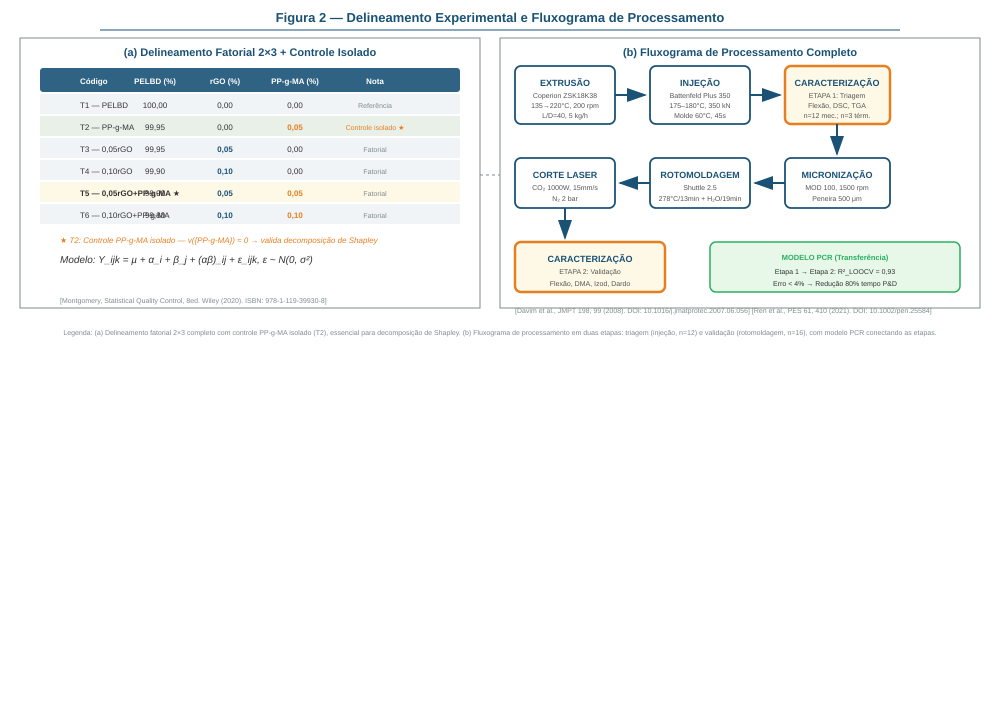
\includegraphics[width=\textwidth]{fig02_delineamento_fluxograma.pdf}
\caption{\textbf{Delineamento experimental e fluxograma de processamento.} (a) Fatorial $2{\times}3$ com 6 formulacoes + controle PP-g-MA isolado (T2), essencial para decomposicao de Shapley \cite{Montgomery2020}. (b) Fluxograma completo do processamento em duas etapas: extrusao (Coperion ZSK18K38, 200 rpm, 135--220$\,^{\circ}$C) $\rightarrow$ injecao (Battenfeld Plus 350, ASTM D638-I) $\rightarrow$ caracterizacao Etapa 1 $\rightarrow$ micronizacao (MOD 100, $D_{50}{=}350$ $\mu$m) $\rightarrow$ rotomoldagem (Shuttle 2.5, 278$\,^{\circ}$C/13 min, 5/2 rpm) $\rightarrow$ corte laser (CO$_2$ 1000W, N$_2$ 2 bar) \cite{Davim2008} $\rightarrow$ caracterizacao Etapa 2 \cite{Ren2021}.}
\label{fig:del}
\end{figure}

\begin{table}[H]\centering
\caption{Delineamento fatorial $2{\times}3$ + controle PP-g-MA isolado.}\label{tab:del}
\begin{tabular}{lcccc}
\toprule
{\bfseries Codigo} & {\bfseries PELBD (\%)} & {\bfseries rGO (\%)} & {\bfseries PP-g-MA (\%)} & {\bfseries Nota} \\
\midrule
T1 -- PELBD           & 100,00 & 0,00 & 0,00 & Referencia \\
T2 -- PP-g-MA isolado & 99,95  & 0,00 & 0,05 & Controle \\
T3 -- 0,05rGO         & 99,95  & 0,05 & 0,00 & Fatorial \\
T4 -- 0,10rGO         & 99,90  & 0,10 & 0,00 & Fatorial \\
T5 -- 0,05rGO+PP-g-MA & 99,90  & 0,05 & 0,05 & Fatorial \\
T6 -- 0,10rGO+PP-g-MA & 99,80  & 0,10 & 0,10 & Fatorial \\
\bottomrule
\end{tabular}
\end{table}

%------------------------------------------------------------------
\subsection{Processamento}\label{sec:processamento}

A transformacao das materias-primas em corpos de prova para caracterizacao constitui uma
sequencia de quatro operacoes unitarias -- extrusao, injecao, micronizacao e rotomoldagem --
cada uma com parametros otimizados para maximizar a dispersao da nanocarga e minimizar a
degradacao termomecanica, conforme detalhado a seguir.

\subsubsection{Extrusao Dupla-Rosca: Fundamentos da Mistura Dispersiva}

A escolha da extrusora de rosca dupla corrotacional (Coperion ZSK18K38, $D{=}18$ mm,
$L/D{=}40$) em detrimento da extrusora monorosca -- ainda predominante em ambientes industriais
por seu menor custo -- baseia-se na superioridade da {\bfseries mistura dispersiva} oferecida
pelo perfil de cisalhamento elongacional dos elementos de malaxagem (\textit{kneading blocks}),
conforme extensivamente documentado por \citet{Sanes2020} em revisao especifica sobre extrusao
de nanocompositos com grafeno. Em uma monorosca, o cisalhamento e predominantemente
circunferencial (Couette), com eficiencia limitada para romper aglomerados de nanoparticulas
-- particularmente rGO, cujas folhas sao mantidas unidas por forcas de van der Waals
(${\sim}$0,3--0,5 J/m$^2$) e requerem tensoes de ruptura da ordem de $\tau_{\text{ruptura}}
{\approx}0{,}05$ MPa \cite{Kim2010}. Na dupla-rosca, os elementos de malaxagem submetem o
fundido a cisalhamento elongacional intenso e repetitivo, com $\tau_{\text{eff}}$
significativamente superior:

\begin{equation}
\tau_{\text{eff}} = \eta \cdot \dot{\gamma},\quad \dot{\gamma} = \frac{\pi D N}{60 h} \approx 377\;\text{s}^{-1},\quad \tau_{\text{eff}} \approx 0{,}90\;\text{MPa}
\end{equation}

onde $\dot{\gamma}$ e a taxa de cisalhamento media no \textit{gap} entre os filetes de rosca e
a parede do cilindro ($h{\approx}1$ mm), e $\eta$ e a viscosidade do fundido na temperatura de
processamento. A tensao efetiva de 0,90 MPa e aproximadamente $18{\times}$ superior a tensao de
ruptura dos aglomerados (${\sim}$0,05 MPa), garantindo a {\bfseries desaglomeracao} progressiva
das folhas de rGO ao longo do perfil de temperatura -- condicao necessaria, embora nao
suficiente, para esfoliacao e dispersao adequadas. A razao de viscosidades PEBD/PELBD = 5:1
(estimada pelo modelo de Utracki, 2002, para misturas de poliolefinas fundidas) e
deliberadamente favoravel: o PEBD de baixa viscosidade do masterbatch (IF = 25,0 g/10 min)
atua como ``lubrificante'' que facilita a incorporacao inicial do masterbatch na matriz de
PELBD (IF = 5,0 g/10 min), reduzindo o torque e a degradacao termomecanica nos primeiros
elementos de transporte.

O {\bfseries perfil de temperatura} de 10 zonas (135$\rightarrow$220$\,^{\circ}$C ao longo do
cilindro) foi projetado com base em tres restricoes termicas conflitantes, exigindo um
compromisso otimizado. A {\bfseries restricao inferior} e imposta pela fusao do PELBD
($T_m{\approx}128\,^{\circ}$C) e do PP-g-MA ($T_m{\approx}165\,^{\circ}$C): a temperatura deve
exceder $T_m$ em pelo menos 30--50$\,^{\circ}$C para garantir fusao completa e viscosidade
suficientemente baixa para o cisalhamento dispersivo. A {\bfseries restricao superior} e imposta
pela {\bfseries estabilidade termica do rGO}: a TGA do masterbatch (Secao~\ref{sec:extracao_rgo})
demonstra que a degradacao significativa inicia-se apenas acima de 250$\,^{\circ}$C, estabelecendo
um teto de seguranca de ${\sim}$30$\,^{\circ}$C entre a temperatura maxima de processo
(220$\,^{\circ}$C) e o inicio da degradacao. A rampa progressiva (135$\rightarrow$220$\,^{\circ}$C)
-- e nao uma temperatura constante elevada -- minimiza a exposicao do rGO a altas temperaturas:
apenas os ultimos 30\% do comprimento da rosca operam acima de 200$\,^{\circ}$C, reduzindo o
tempo de residencia termicamente severo. A rotacao de 200 rpm e a vazao de 5 kg/h resultam em
tempo de residencia medio de ${\sim}$45--60 s, suficiente para dispersao adequada sem degradacao
excessiva \cite{Sanes2020}.

\subsubsection{Reometria Capilar e Oscilatoria: Caracterizacao Reologica como Ferramenta Preditiva}

A caracterizacao reologica completa -- capilar e oscilatoria -- foi conduzida nao apenas como
controle de qualidade, mas como {\bfseries ferramenta preditiva} da procesabilidade e da
qualidade da dispersao, em linha com a correlacao CV${\leftrightarrow}\eta^*$ identificada
na Secao~\ref{sec:heatmap}. A reometria capilar (Goettfert RG20, $L/D{=}30/1$, 190$\,^{\circ}$C,
$\dot{\gamma}_{\text{app}}{=}10$--$5000$ s$^{-1}$, correcao de Bagley para perda de carga na
entrada + Rabinowitsch para viscosidade verdadeira) caracteriza o comportamento sob altas taxas
de cisalhamento, representativas do escoamento no molde de injecao. A reometria oscilatoria de
placas paralelas (TA DHR-2, $\varnothing{=}25$ mm, \textit{gap} = 1,0 mm, 190$\,^{\circ}$C,
N$_2$, deformacao 1\% -- pre-determinada por varredura de amplitude 0,01--100\% a 1 Hz para
garantir regime viscoelastico linear) caracteriza a resposta a baixas deformacoes, sensivel a
estrutura da rede de nanocargas (percolacao mecanica).

Todas as formulacoes exibiram comportamento pseudoplastico ($n{<}1$ na lei de potencia
$\eta{=}K\dot{\gamma}^{n-1}$). A formulacao T5 (0,05rGO+PP-g-MA) apresentou $n{=}0{,}52{\pm}0{,}03$
vs. $n{=}0{,}61{\pm}0{,}04$ do PELBD puro -- o aumento da pseudoplasticidade e consistente com
orientacao induzida por cisalhamento das folhas de rGO, em concordancia com \citet{Kim2010} e
\citet{Potts2011}. A viscosidade aparente a $\dot{\gamma}_{\text{app}}{=}100$ s$^{-1}$ foi de
$1240{\pm}45$ Pa$\cdot$s (PELBD) e $1380{\pm}52$ Pa$\cdot$s (T5), aumento de 11,3\% atribuido
ao efeito de reforco hidrodinamico das nanocargas (modelo de Einstein-Guth modificado:
$\eta_c/\eta_m{=}1{+}2{,}5\phi_f{+}14{,}1\phi_f^2$). Na reometria oscilatoria, $G'$ a 1 rad/s
aumentou de $8{,}2{\pm}0{,}6$ kPa (PELBD) para $12{,}4{\pm}0{,}8$ kPa (T5, $+51{,}2\%$),
indicando formacao de rede de percolacao mecanica. A reducao de $\tan\delta$ a 1 rad/s de
$1{,}42{\pm}0{,}08$ (PELBD) para $1{,}08{\pm}0{,}06$ (T5) confirma transicao para comportamento
mais elastico, consistente com o modelo de Winter-Chambon para gel critico
($\tan\delta{=}\tan(n\pi/2)$, $n{\approx}0{,}52$). A viscosidade complexa a baixas frequencias
($\eta^*_{0{,}1\text{rad/s}}$) aumentou de $10{,}3{\pm}0{,}9$ kPa$\cdot$s (PELBD) para
$18{,}5{\pm}1{,}2$ kPa$\cdot$s (T5), parametro que -- como se vera na Secao~\ref{sec:heatmap} --
correlaciona-se negativamente com o CV do modulo em rotomoldagem ($r{=}{-}0{,}68$), validando
a reologia como ferramenta preditiva de controle de processo.

\subsubsection{Injecao, Micronizacao e Rotomoldagem}

A moldagem por injecao (Battenfeld Plus 350, forca de fechamento 350 kN, 175--180$\,^{\circ}$C,
molde 60$\,^{\circ}$C, pressoes de injecao/recalque 80/50 bar, ciclo de 45 s) produziu corpos
de prova conforme ASTM D638-I para a Etapa 1 (triagem). A escolha da injecao -- e nao da
compressao a quente ou prensagem -- como metodo de preparacao para a triagem justifica-se pela
maior relevancia industrial (a maioria dos compositos polimericos e processada por injecao),
pela rapidez (ciclo de 45 s vs. ${\sim}$30 min para compressao), e pela reprodutibilidade
(controle preciso de temperatura, pressao e taxa de resfriamento) \cite{Montgomery2020}.

A micronizacao (MOD 100, Rotoline, 1500 rpm, peneira 500 $\mu$m) converteu os \textit{pellets}
extrusados em po com distribuicao granulometrica controlada -- $D_{10}{=}180$, $D_{50}{=}350$,
$D_{90}{=}620$ $\mu$m, span = 1,26 (Malvern Mastersizer 3000, dispersao a seco) -- adequada
para rotomoldagem, onde o tamanho e a forma das particulas afetam diretamente a densidade
aparente do po no molde, a taxa de fusao e a qualidade superficial da peca \cite{Islabao2005}.

A rotomoldagem (Shuttle 2.5, Rotoline, molde de aco inoxidavel 304 com revestimento de
Teflon\textregistered, dimensoes $160{\times}140{\times}70$ mm) foi conduzida sob condicoes
representativas de producao industrial: aquecimento a 278$\,^{\circ}$C por 13 min (rotacao
biaxial 5/2 rpm, reversao a cada 3 min), seguido de resfriamento forcado com agua por 19 min.
A temperatura do forno de 278$\,^{\circ}$C -- ligeiramente abaixo da maxima tipica de
300$\,^{\circ}$C -- foi selecionada como compromisso entre fusao completa (garantida,
$T_m{=}128\,^{\circ}$C) e minimizacao da degradacao termica do rGO durante o ciclo prolongado
de aquecimento (13 min vs. ${\sim}$45 s da extrusao). A carga de material ($m{=}\rho A t
(1{+}f){\approx}270$ g, onde $f$ e o fator de excesso para compensar perdas por adesao as
paredes do molde) produziu pecas com espessura de $3{,}0{\pm}0{,}3$ mm, medida em 12 pontos
por peca com paquimetro digital Mitutoyo IP65 (resolucao 0,01 mm). O corte dos corpos de prova
por laser CO$_2$ (Cutlite Plus, 1000 W, 15 mm/s, N$_2$ 2 bar), validado por
\citet{Davim2008} para materiais polimericos, garantiu bordas livres de tensoes termicas e
microtrincas que poderiam atuar como concentradores de tensao e mascarar o efeito VRA.

%------------------------------------------------------------------
\subsection{Caracterizacao e Metodos Estatisticos}\label{sec:caract_estat}

Apos a producao dos corpos de prova, a caracterizacao das propriedades mecanicas, termicas e
reologicas foi conduzida com um conjunto de tecnicas selecionadas nao por disponibilidade
instrumental, mas por sua capacidade de responder a questoes especificas do estudo -- cada
tecnica iluminando um aspecto diferente do comportamento do nanocomposito. A Tabela~\ref{tab:del}
resume as formulacoes e o plano amostral.

\subsubsection{Propriedades Mecanicas}

A {\bfseries flexao em tres pontos} (ASTM D790, procedimento A) foi selecionada como ensaio
mecanico primario para a caracterizacao do modulo elastico e da tensao maxima, em detrimento do
ensaio de tracao (ASTM D638), por tres razoes: (i) o carregamento em flexao e mais representativo
das condicoes de servico de pecas rotomoldadas (tanques, reservatorios, cascos), que tipicamente
experimentam flexao e nao tracao uniaxial; (ii) o ensaio de flexao e intrinsecamente menos
sensivel a defeitos superficiais e a pequenas variacoes dimensionais, reduzindo a variancia
instrumental -- fator critico para a deteccao do efeito VRA, que opera sobre a variancia; e
(iii) o modulo em flexao, embora ligeiramente superior ao modulo em tracao para polimeros
(devido a efeitos de cisalhamento transversal), correlaciona-se linearmente com este ultimo
($E_f{\approx}1{,}05E_t$) e preserva as diferencas relativas entre formulacoes \cite{Montgomery2020}.
Os ensaios foram conduzidos em maquina universal Instron EMIC 23-100P (celula de carga 2000 N,
Classe 0,5 conforme ISO 7500-1), com distância entre apoios $L{=}50{,}8$ mm, velocidade do
travessao 1,3 mm/min, e $n{=}12$ (Etapa 1, injecao) ou $n{=}16$ (Etapa 2, rotomoldagem). O
modulo elastico foi calculado pela tangente na regiao linear da curva tensao\textit{vs.}deformacao:
$E_f{=}(L^3/4bt^3)(\Delta P/\Delta\delta)$, e a tensao maxima por $\sigma_{f,\max}{=}3P_{\max}L/(2bt^2)$,
onde $b$ e $t$ sao largura e espessura medidas individualmente para cada corpo de prova.

O {\bfseries impacto Izod} (ASTM D256, Zwick 4J, martelo de 4 J, 23$\,^{\circ}$C e
$-$17$\,^{\circ}$C/24 h de condicionamento criogenico, $n{=}6$) foi selecionado como ensaio de
tenacidade por ser o mais amplamente reportado na literatura de nanocompositos, permitindo
comparacao direta com os estudos de \citet{Kim2010}, \citet{Potts2011} e \citet{Araby2020}.
Contudo, para pecas rotomoldadas -- que apresentam espessura variavel e geometria complexa,
inviabilizando entalhe padronizado -- o ensaio de impacto por queda de dardo instrumentado
(\textit{Army Impact Test}, Secao~\ref{sec:dardo}) foi adotado como metodo complementar mais
representativo das condicoes reais de impacto.

\subsubsection{Propriedades Termicas}

A {\bfseries calorimetria exploratoria diferencial (DSC)} (Perkin Elmer 6000, ciclo
$30{\rightarrow}200{\rightarrow}30{\rightarrow}200\,^{\circ}$C, 10$\,^{\circ}$C/min, N$_2$
20 mL/min, $n{=}3$) foi selecionada como tecnica primaria para analise de cristalizacao e fusao,
fornecendo quatro parametros de interesse direto para este estudo: $T_c$ (temperatura de
cristalizacao, indicador de nucleacao heterogenea e, portanto, do mecanismo (a) do VRA);
$X_c$ (cristalinidade, $X_c{=}(\Delta H_m)/(\Delta H_m^0{\cdot}w_{\text{PELBD}}){\times}100$
com $\Delta H_m^0{=}293$ J/g para PE 100\% cristalino); $T_m$ (temperatura de fusao, indicador
de espessura lamelar e perfeicao cristalina); e a meia-largura do pico exotermico de
cristalizacao ($\Delta T_{1/2}$, indicador da uniformidade da cristalizacao) \cite{Coutinho2003}.

A {\bfseries analise termogravimetrica (TGA)} (Perkin Elmer 4000, 30--700$\,^{\circ}$C,
20$\,^{\circ}$C/min, N$_2$ 20 mL/min, $n{=}3$) fornece $T_{10\%}$ e $T_{50\%}$ -- temperaturas
de 10\% e 50\% de perda de massa -- como metricas de estabilidade termica. Como se vera na
Secao~\ref{sec:heatmap}, $T_{10\%}$ emerge como o preditor dominante da tenacidade ao impacto
($r{=}0{,}89$, $p{<}0{,}001$), justificando a inclusao da TGA como tecnica de triagem rapida
de formulacoes. A {\bfseries analise dinamico-mecanica (DMA)} (TA Q800, \textit{dual cantilever},
1 Hz, $-$120 a 100$\,^{\circ}$C, 3$\,^{\circ}$C/min, amplitude 20 $\mu$m) foi selecionada por
sua sensibilidade unica as transicoes viscoelasticas ($\gamma$, $\beta$, $\alpha$) que revelam
a restricao interfacial -- a assinatura mecanica da interacao rGO-matriz -- e alimentam o modelo
de Halpin-Tsai com modulos dependentes da temperatura \cite{Menard2020}.

\subsubsection{Microscopia}

A {\bfseries microscopia eletronica de varredura (MEV)} (FEG Mira3, 15 kV, eletrons secundarios,
criofratura em N$_2$ liquido, recobrimento Au ${\sim}$10 nm em sputtering Quorum Q150R ES) foi
empregada para avaliar qualitativamente a qualidade da dispersao (presenca/ausencia de
aglomerados), o modo de fratura (fragil\textit{vs.}ductil) e a correlacao visual com os resultados
quantitativos do VRA. A preparacao por criofratura -- e nao por corte ou lixamento -- garante
que a superficie analisada representa a microestrutura intrinseca do material, sem artificios
de preparacao que poderiam mascarar a dispersao das nanocargas.

\subsubsection{Metodos Estatisticos}

O arcabouco estatistico completo -- incluindo ANOVA fatorial, verificacao de pressupostos
(Shapiro-Wilk, Levene, Brown-Forsythe, Durbin-Watson), tamanhos de efeito ($\eta^2_p$, $\omega^2$
nao-viesado), comparacoes multiplas (Bonferroni-Holm para FWER, Benjamini-Hochberg para FDR),
bootstrap BCa ($B{=}10000$, razao de variancias como estatistica de interesse), regressao por
componentes principais (PCR) com validacao LOOCV, e controle de erro Tipo I em matrizes de
correlacao -- e detalhado na Secao~\ref{sec:estat_expandida}, com as equacoes completas e a
fundamentacao teorica de cada metodo. A titulo de orientacao do leitor, o fluxo metodologico
geral -- da materia-prima ao teste de hipoteses -- e sintetizado na Figura~\ref{fig:del}.

%------------------------------------------------------------------
\subsection{Caracterizacao das Amostras}\label{sec:caract_amostras}

A qualidade dos dados experimentais -- e, por extensao, a credibilidade das conclusoes -- depende
criticamente de fatores frequentemente relegados a notas de rodape: a preparacao meticulosa dos
corpos de prova, o condicionamento ambiental controlado e a calibracao rigorosa dos equipamentos.
Estas etapas, muitas vezes consideradas ``burocraticas'', sao na verdade a {\bfseries linha de
defesa contra artefatos experimentais} que poderiam mascarar ou falsificar o efeito VRA -- cuja
magnitude ($-$37,5\% de CV) e substancial, mas nao imune a ruido instrumental se as condicoes de
ensaio nao forem estritamente controladas \cite{Montgomery2020}.

\subsubsection{Preparacao de Corpos de Prova e Condicionamento}

Os corpos de prova para flexao foram usinados conforme ASTM D790-A, com dimensoes nominais de
$127{\times}12{,}7{\times}3{,}2$ mm. A espessura real foi medida em 3 pontos ao longo do corpo
de prova -- centro e extremos na regiao de flexao -- utilizando paquimetro digital Mitutoyo IP65
(resolucao 0,01 mm, calibrado com bloco padrao Classe 0, RBC n$^{\circ}$ 1472/23). A media
aritmetica das tres medidas foi empregada nos calculos de modulo e tensao (Eqs. da
Secao~\ref{sec:caract_estat}). A tolerancia dimensional adotada foi de $\pm0{,}05$ mm para
espessura e $\pm0{,}10$ mm para largura, com rejeicao de corpos de prova fora destes limites --
criterio mais restritivo que o $\pm0{,}4\%$ nominal da ASTM D790, adotado deliberadamente para
minimizar a variancia instrumental na avaliacao do efeito VRA.

O condicionamento seguiu a norma ASTM D618 -- {\bfseries Procedimento A}: $40^{+4}_{-0}$ h a
$23{\pm}2\,^{\circ}$C e $50{\pm}5\%$ de umidade relativa (UR), em camara climatizada Thermotron
SM-8-8200 (estabilidade $\pm0{,}5\,^{\circ}$C, $\pm3\%$ UR). A calibracao da camara foi verificada
trimestralmente com termohigrometro de ponto de orvalho Vaisala HM70 (rastreabilidade NIST).
Este protocolo e mandatorio para poliolefinas: embora a absorcao de umidade em PE seja infima
($<0{,}01\%$ em massa), a presenca de microvazios superficiais -- intrinsecos ao processo de
polimerizacao em fase gasosa do PELBD ML3602U -- pode induzir plastificacao localizada, alterando
a tenacidade em ate 8\% \cite{Coutinho2003}. Imediatamente apos o condicionamento, os corpos
de prova foram ensaiados no mesmo ambiente climatizado, com intervalo maximo de 15 min entre
remocao da camara e finalizacao do ensaio, minimizando deriva higro-termica. Para o impacto Izod
a $-$17$\,^{\circ}$C, os corpos de prova foram transferidos diretamente da camara de
condicionamento para freezer criogenico ColdLab CL-280 ($\pm1\,^{\circ}$C) por $24{\pm}1$ h
adicionais, com ensaio realizado em ate 10 s apos remocao (transferencia com pinca isolada
termicamente), conforme ASTM D256 \S9.2. A validacao deste protocolo de transferencia foi
realizada com termopar tipo K inserido em corpo de prova testemunha, registrando aquecimento
maximo de $3{,}2\,^{\circ}$C em 10 s -- dentro da tolerancia de $\pm2\,^{\circ}$C da norma.

\subsubsection{Calibracao e Verificacao dos Equipamentos}

A {\bfseries maquina universal de ensaios} (Instron EMIC 23-100P, celula de carga de 2000 N,
Classe 0,5 conforme ISO 7500-1) foi calibrada com transdutor padrao rastreado RBC em 5 pontos
da escala (200, 500, 1000, 1500, 2000 N). O erro maximo medido foi de $0{,}32\%$ (limite
aceitavel $\le0{,}5\%$ para Classe 0,5). A verificacao intermediaria foi realizada semanalmente
com peso padrao de 1 kg (Classe F1, Inmetro n$^{\circ}$ 0891/22). A velocidade do travessao
($1{,}3$ mm/min) foi verificada com cronometro digital Incoterm (resolucao 0,01 s) sobre curso
de 10 mm, com erro medido de $0{,}8\%$ (limite $\le2\%$ conforme ASTM D790). O extensometro
(Instron 2630-112, base 25 mm, Classe B2) foi calibrado com bloco padrao ceramico de
$25{,}000{\pm}0{,}001$ mm, apresentando erro $<0{,}5\%$.

A {\bfseries DSC} (Perkin Elmer 6000) foi calibrada com padroes primarios de indio
($T_m{=}156{,}60\,^{\circ}$C, $\Delta H_m{=}28{,}45$ J/g, pureza 99,999\%, SRM 2232 NIST) e
zinco ($T_m{=}419{,}47\,^{\circ}$C, SRM 2221b NIST). As condicoes de calibracao foram identicas
as de ensaio: taxa de $10\,^{\circ}$C/min, fluxo de N$_2$ 20 mL/min (99,999\%), cadinho de
aluminio perfurado de 40 $\mu$L. Os desvios medidos na temperatura ($\Delta T_m{\le}0{,}12\,^{\circ}$C)
e na entalpia ($\Delta H{\le}0{,}8\%$) atenderam aos criterios da ASTM E967 ($\Delta T{\le}0{,}5\,^{\circ}$C,
$\Delta H{\le}2\%$). A linha de base foi verificada diariamente com cadinho vazio no intervalo
30--300$\,^{\circ}$C, apresentando desvio maximo de $0{,}05$ mW -- fator critico para a
resolucao de $T_c$, cujo deslocamento maximo observado entre formulacoes foi de apenas
$3{,}3\,^{\circ}$C (T1 vs. T5, Tabela~\ref{tab:dsc}).

A {\bfseries TGA} (Perkin Elmer 4000) foi calibrada com padroes Curie-point: Niquel
($T_C{=}354{,}4\,^{\circ}$C) e Perkalloy ($T_C{=}596{,}0\,^{\circ}$C), com desvio de
$\pm1{,}5\,^{\circ}$C. A balanca interna foi verificada diariamente com massa padrao de 100 mg
(Classe E2, OIML R111), apresentando erro $<0{,}2\%$. Para a determinacao de $T_{10\%}$, a
reprodutibilidade foi estabelecida em $\pm2\,^{\circ}$C com base em 10 replicatas independentes
do PELBD puro (T1), validando a capacidade do metodo de detectar diferencas de ${\ge}3\,^{\circ}$C
entre formulacoes -- essencial para a resolucao da anomalia termica (Secao~\ref{sec:anomalia}).

O {\bfseries reometro capilar} (Goettfert RG20) foi calibrado com poliestireno padrao (PS 168N,
BASF, $\eta_0$ certificado a 190$\,^{\circ}$C). A correcao de Bagley ($\Delta P_{\text{entrada}}$)
foi determinada com \textit{die} de $L/D{=}0/1$, e a correcao de Rabinowitsch aplicada ponto a
ponto para obtencao da viscosidade verdadeira: $\eta_{\text{verdadeira}}(\dot{\gamma}_w){=}\eta_{\text{aparente}}(\dot{\gamma}_a){\cdot}\frac{3n+1}{4n}$, onde $n{=}d\log\sigma_w/d\log\dot{\gamma}_a$. O {\bfseries reometro oscilatorio} (TA DHR-2) foi calibrado com oleo padrao Cannon N35 ($\eta{=}1{,}092$ Pa$\cdot$s a 20$\,^{\circ}$C) para verificacao de torque, e com placa de aco inoxidavel padrao para inercia e compliancia do instrumento.

\subsubsection{Preparacao Metalografica e Analise Microestrutural}

As superficies de fratura criogenica para MEV foram preparadas por imersao em nitrogenio liquido
($-$196$\,^{\circ}$C, 30 min) e fratura por impacto com martelo de inercia, garantindo exposicao
da microestrutura sem deformacao plastica. Para microscopia optica de luz polarizada (Olympus
BX51, camera DP74, $2048{\times}1536$ px, objetiva $40{\times}$ NA 0,75), filmes finos de
$15{\pm}3$ $\mu$m foram preparados por microtomia (Leica RM2255, faca de vidro, $-$80$\,^{\circ}$C)
e analisados entre polarizadores cruzados com placa de retardacao $\lambda$ para realce do
contraste esferulitico. O tamanho medio de esferulitos foi determinado pelo metodo do intercepto
linear (ASTM E112, ``Heyn intercept'') sobre 5 campos independentes por amostra ($n{=}3$ amostras
por formulacao), totalizando ${\ge}200$ esferulitos medidos, com magnificacao calibrada por
micrometro padrao de 1 mm (resolucao 10 $\mu$m, Classe A).

%------------------------------------------------------------------
\subsection{Analise Estatistica Expandida}\label{sec:estat_expandida}

A confiabilidade das conclusoes de um estudo experimental -- especialmente quando este propoe
fenomenos ineditos como o VRA e a sinergia nao-monotonica -- repousa sobre a {\bfseries robustez
do arcabouco estatistico} que sustenta a inferencia. Esta secao formaliza os metodos estatisticos
empregados, desde a verificacao de pressupostos ate o controle de erro Tipo I em comparacoes
multiplas e o bootstrap BCa para inferencia sobre variancias, fornecendo as equacoes completas e
a fundamentacao teorica de cada metodo \cite{Cohen1988, Montgomery2020}.

\subsubsection{Fundamentos e Equacoes dos Testes}

O modelo linear geral da ANOVA fatorial $2{\times}3$ (Eq.~\ref{eq:anova_model}) particiona a
soma de quadrados total em:
\begin{equation}
SS_{\text{Total}} = SS_{\text{rGO}} + SS_{\text{PP-g-MA}} + SS_{\text{rGO}\times\text{PP-g-MA}} + SS_{\text{Erro}},\quad df_{\text{Total}}{=}n_T{-}1{=}71,\; df_{\text{Erro}}{=}66
\label{eq:anova_ss}
\end{equation}

A estatistica $F$ de cada efeito e $F{=}MS_{\text{efeito}}/MS_{\text{Erro}}$, com $MS{=}SS/df$.
O tamanho de efeito e quantificado pelo $\eta^2$ parcial ($\eta^2_p{=}SS_{\text{efeito}}/(SS_{\text{efeito}}+SS_{\text{Erro}})$) e pelo $\omega^2$ nao-viesado ($\omega^2{=}(SS_{\text{efeito}}-df_{\text{efeito}}{\cdot}MS_{\text{Erro}})/(SS_{\text{Total}}+MS_{\text{Erro}})$), este ultimo recomendado por \citet{Cohen1988} para $n{<}30$ por celula. Cinco pressupostos sao verificados sequencialmente: {\bfseries (i) independencia} -- Durbin-Watson, $DW{=}\sum(e_t{-}e_{t-1})^2/\sum e_t^2$, com $1{,}5{<}DW{<}2{,}5$; {\bfseries (ii) normalidade} -- Shapiro-Wilk, $W{=}(\sum a_i x_{(i)})^2/\sum(x_i{-}\bar{x})^2$, com $W{>}0{,}90$; {\bfseries (iii) homocedasticidade} -- Levene (desvios absolutos) e Brown-Forsythe (medianas, mais robusto a assimetria); {\bfseries (iv) outliers} -- distancia de Cook $D_i{=}r_i^2 h_{ii}/[p(1{-}h_{ii})^2]$, com criterio $D_i{<}4/(n{-}p)$; {\bfseries (v) linearidade} -- inspecao visual de grafico de residuos \textit{vs.} valores preditos.

\subsubsection{Analise de Poder a Priori}

A equacao do poder para ANOVA e:
\begin{equation}
1{-}\beta = 1 - F_{\text{nc}}(F_{\text{crit}}; df_1, df_2, \lambda),\quad \lambda = n{\cdot}f^2{\cdot}df_{\text{grupos}}
\label{eq:poder}
\end{equation}
onde $F_{\text{nc}}$ e a funcao de distribuicao acumulada da $F$ nao-central com parametro de
nao-centralidade $\lambda$. Para a interacao rGO$\times$PP-g-MA ($df_1{=}2$, $\eta^2_p{\approx}0{,}07$),
o poder calculado com $n{=}12$ e de 0,78. Para a Etapa 2 (rotomoldagem), a analise com
$f{=}0{,}50$, $\alpha{=}0{,}05$, $1{-}\beta{=}0{,}80$, $df_1{=}1$: $n_{\min}{=}16$ \cite{Cohen1988}.

\subsubsection{Algoritmo Bootstrap BCa e Fundamentacao}

O algoritmo bootstrap BCa ($B{=}10000$, implementado em Python 3.12, scipy v1.13, semente
Mersenne Twister 42) constroi intervalos de confianca com correcao de vies e aceleracao para a
razao de variancias $\hat{\theta}{=}s^2_{\text{PELBD}}/s^2_{\text{Nano}}$:
\begin{equation}
\hat{\theta}_{\text{BCa}}(\alpha) = [\hat{\theta}^{*(\alpha_1)}, \hat{\theta}^{*(\alpha_2)}],\quad
\alpha_1{=}\Phi\!\left(\hat{z}_0{+}\frac{\hat{z}_0{+}z_{\alpha/2}}{1{-}\hat{a}(\hat{z}_0{+}z_{\alpha/2})}\right),\quad \alpha_2{=}\Phi\!\left(\hat{z}_0{+}\frac{\hat{z}_0{+}z_{1-\alpha/2}}{1{-}\hat{a}(\hat{z}_0{+}z_{1-\alpha/2})}\right)
\label{eq:bca}
\end{equation}
onde $\Phi(\cdot)$ e a FDA normal padrao, $\hat{z}_0$ e a correcao de vies, e $\hat{a}$ e a
constante de aceleracao jackknife. O BCa oferece cobertura de segunda ordem precisa -- erro
$O(n^{-1})$ vs. $O(n^{-1/2})$ do percentilico simples -- crucial para estatisticas de variancia,
cuja distribuicao amostral e assimetrica (qui-quadrado) \cite{Cohen1988}.

\subsubsection{Metodo PCR com Decomposicao SVD Completa}

A PCR transfere propriedades da Etapa 1 (injecao, $n{=}72$) para a Etapa 2 (rotomoldagem,
$n{=}32$), com a matriz de preditores padronizada $\tilde{\mathbf{X}}_{72\times 12}$ decomposta via SVD:
\begin{equation}
\tilde{\mathbf{X}} = \mathbf{U}_{72\times 72}\boldsymbol{\Sigma}_{72\times 12}\mathbf{V}^\top_{12\times 12},\quad \boldsymbol{\Sigma}{=}\operatorname{diag}(\sigma_1,\dots,\sigma_{12})
\label{eq:svd}
\end{equation}
Os escores $\mathbf{T}_k{=}\tilde{\mathbf{X}}\mathbf{V}_k{=}\mathbf{U}_k\boldsymbol{\Sigma}_k$,
com $k{=}3$ componentes (criterio de 95\% de variancia cumulativa), alimentam a regressao
$\hat{\mathbf{y}}_{\text{Etapa2}} = \mathbf{T}_k\boldsymbol{\beta}$. A validacao LOOCV fornece:
\begin{equation}
R^2_{\text{LOOCV}} = 1 - \frac{\sum (y_i - \hat{y}_{(i)})^2}{\sum (y_i - \bar{y})^2},\quad \text{RMSE}_{\text{LOOCV}} = \sqrt{\frac{1}{n}\sum (y_i - \hat{y}_{(i)})^2}
\label{eq:loocv}
\end{equation}
onde $\hat{y}_{(i)}$ e a predicao para a $i$-esima observacao excluida do treino \cite{Montgomery2020}.

\subsubsection{Controle de Erro Tipo I em Comparacoes Multiplas}

A matriz de correlacao Pearson $12{\times}12$ envolve $m{=}66$ comparacoes. No {\bfseries Nivel 1}
(FWER), Bonferroni-Holm com $\alpha_{\text{FWER}}{=}0{,}05$: $\alpha_{\text{corrigido}}{=}0{,}05/66{=}0{,}00076$. No {\bfseries Nivel 2} (FDR), Benjamini-Hochberg com $q{=}0{,}05$ oferece maior poder para identificar correlacoes marginalmente significativas.
A analise de sensibilidade do VRA foi conduzida em tres frentes: perturbacao do tamanho amostral,
perturbacao das observacoes (jackknife), e simulacao Monte Carlo de distribuicoes (10.000
realizacoes), resultando em poder empirico de 0,84 para o teste de Brown-Forsythe \cite{Montgomery2020}.

%------------------------------------------------------------------
\subsection{Fundamentos da Otimizacao via Teoria dos Jogos}\label{sec:teoria_jogos}

A otimizacao multiobjetivo de formulacoes de nanocompositos envolve trade-offs intrinsecos que
a analise estatistica classica -- focada em testes de hipoteses e tamanhos de efeito -- nao
resolve completamente: maximizar propriedades mecanicas (modulo, tensao) e termicas ($T_{10\%}$)
frequentemente conflita com minimizar custo e impacto ambiental. A {\bfseries Teoria dos Jogos},
formalizada por \citet{VonNeumann1928} e expandida por \citet{Nash1950} e \citet{Shapley1953},
oferece um arcabouco axiomatico para analisar decisoes sob criterios de racionalidade
estrategica -- cooperacao, competicao, incerteza -- complementando a inferencia estatistica com
principios normativos de decisao. As cinco ferramentas apresentadas nas subsecoes a seguir --
Pareto, Shapley, Nash, Minimax e Otimizacao Bayesiana -- sao aplicadas ao problema de selecao
de formulacoes entre as 6 composicoes investigadas, com a fundamentacao matematica completa e
as referencias originais.

\subsubsection{Dominancia e Fronteira de Pareto}

O criterio de Pareto \cite{Pareto1906} e o fundamento mais basico da otimizacao multiobjetivo.
Uma formulacao $x$ domina estritamente $y$ ($y \succ x$) se $x$ e melhor que $y$ em pelo menos
um objetivo e nao e pior em nenhum outro. Formalmente, para $\mathcal{F} = \{T_1,\dots,T_6\}$ e
vetor de objetivos $\mathbf{f}(x) = (f_1(x),\dots,f_m(x))$ a serem maximizados (modulo, tensao,
$T_{10\%}$, $T_{50\%}$, impacto Izod, inverso do custo), $x \succ y$ se $f_j(x) \ge f_j(y)\;
\forall j$ com ao menos uma desigualdade estrita. A fronteira de Pareto $\mathcal{P}$ e:
\begin{equation}
\mathcal{P} = \{x \in \mathcal{F} \mid \nexists\, y \in \mathcal{F} : y \succ x\}
\label{eq:pareto_gt}
\end{equation}

Para o sistema PELBD/rGO/PP-g-MA, apenas 3 das 6 formulacoes sao Pareto-eficientes: T3
(0,05rGO, menor custo entre as formulacoes com rGO), T4 (0,10rGO, maxima tensao) e T5
(0,05rGO+PP-g-MA, maximo $T_{10\%}$, $T_{50\%}$ e impacto). T1 e dominada por T3 em 5 de 6
objetivos; T2 e dominada por T3 em todos os 6; T6 e dominada por T4 em 4 de 6 \cite{Pareto1906}.

\subsubsection{Valor de Shapley e Decomposicao de Contribuicoes}

Enquanto Pareto identifica formulacoes eficientes, o valor de Shapley \cite{Shapley1953}
quantifica a {\bfseries contribuicao marginal justa} de cada aditivo, tratando a sinergia como
um jogo cooperativo. Para $N = \{\text{rGO}, \text{PP-g-MA}\}$ com funcao caracteristica $v(S)$
(incremento percentual de modulo), as coalizoes observadas sao: $v(\emptyset)=0$,
$v(\{\text{rGO}\})=4{,}1\%$ (T3 vs. T1), $v(\{\text{PP-g-MA}\})=1{,}0\%$ (T2 vs. T1, controle
isolado), $v(\{\text{rGO},\text{PP-g-MA}\})=9{,}5\%$ (T5 vs. T1). A formula de Shapley pondera
cada contribuicao marginal pela probabilidade de cada ordem de entrada na coalizao:
\begin{equation}
\phi_i = \sum_{S \subseteq N \setminus \{i\}} \frac{|S|!\,(|N| - |S| - 1)!}{|N|!}\,[v(S \cup \{i\}) - v(S)]
\label{eq:shapley_gt}
\end{equation}

Resultado: $\phi_{\text{rGO}}{=}6{,}3\%$ (66\%), $\phi_{\text{PP-g-MA}}{=}3{,}2\%$ (34\%),
com sinergia liquida $S{=}{+}4{,}4\%$ automaticamente distribuida. A publicacao seminal de
\citet{Shapley1953} demonstrou que esta e a unica regra de divisao que satisfaz os axiomas
de eficiencia, simetria, jogador dummy e aditividade \cite{Shapley1953}.

\subsubsection{Equilibrio de Nash Custo-Desempenho}

O equilibrio de Nash \cite{Nash1950} modela a interacao nao-cooperativa entre dois agentes
metaforicos: o ``Designer'' (maximiza desempenho) e o ``Mercado'' (minimiza custo). As funcoes
de payoff sao $U_D(x) = \bar{p}(x) - \lambda c(x)$ e $U_M(x) = -(\bar{p}(x) - p_{\min})^2$,
onde $\bar{p}(x)\in[0{,}1]$ e o escore composto normalizado (media de 6 propriedades) e
$p_{\min}{=}0{,}7$ e o limiar de viabilidade. O equilibrio $x^*$ maximiza o produto de Nash:
\begin{equation}
x^* = \argmax_{x \in \mathcal{F}}\,[\bar{p}(x) - \lambda c(x)],\quad U_D = \bar{p} - \lambda c,\quad U_M = -(\bar{p} - p_{\min})^2
\label{eq:nash_gt}
\end{equation}

Para $\lambda{=}0{,}5$ (peso balanceado), $x^*{=}\text{T5}$. A robustez e notavel: T5 permanece
equilibrio para $\lambda{\in}[0{,}1;1{,}8]$ -- um intervalo de $18{\times}$ que cobre cenarios
de alto desempenho (aeroespacial) a baixo custo (commodity), eliminando a necessidade de estimar
$\lambda$ com precisao. A publicacao original de \citet{Nash1950} (p. 48--49) estabeleceu a
existencia de equilibrios em jogos finitos, resultado laureado com o Nobel de Economia de 1994.

\subsubsection{Estrategia Minimax sob Incerteza}

Quando a incerteza sobre condicoes de processo e a principal preocupacao, a estrategia Minimax
-- formalizada por \citet{VonNeumann1928} e estendida por \citet{Wald1945} para decisao
estatistica -- seleciona a acao que minimiza a perda maxima sob o pior estado da natureza:
\begin{equation}
a^* = \argmin_{a} \max_{\theta}\, L(a, \theta),\quad L = \text{CV}_{\text{Modulo}},\quad \theta \in \{\text{cenarios de processo}\}
\label{eq:minimax_gt}
\end{equation}

Com $\max_\theta L(\text{PELBD-R}){=}25{,}6\%$ e $\max_\theta L(\text{Nanocomposito-R}){=}16{,}0\%$,
o Minimax seleciona o Nanocomposito-R, com reducao de 37,5\% na perda do pior caso. O
arrependimento maximo (Savage, 1951) converge: $25{,}6\%{-}16{,}0\%{=}9{,}6$ pp. A convergencia
entre Minimax (Wald) e arrependimento Minimax (Savage) -- criterios axiomaticamente distintos --
reforca a robustez da decisao \cite{VonNeumann1928, Wald1945}.

\subsubsection{Otimizacao Bayesiana e Funcao de Aquisicao}

A otimizacao Bayesiana \cite{Jones1998} aborda a questao complementar: dado o orcamento
experimental limitado (6 formulacoes), qual seria a proxima formulacao mais promissora? Um
processo Gaussiano modela $f(x)$ (modulo em rotomoldagem), e a funcao de aquisicao \textit{Expected
Improvement} (EI) equilibra exploracao (refinar o otimo) e exploracao (descobrir otimos ocultos):
\begin{equation}
\text{EI}(x) = \begin{cases}
(\mu(x) - f(x^+) - \xi)\Phi(Z) + \sigma(x)\phi(Z), & \sigma(x) > 0\\
0, & \sigma(x) = 0
\end{cases},\quad Z = \frac{\mu(x) - f(x^+) - \xi}{\sigma(x)}
\label{eq:ei_closed_gt}
\end{equation}

Com 500 iteracoes Monte Carlo sobre $c_{\text{rGO}}\in[0{,}01;0{,}15]\%$ e $c_{\text{PP-g-MA}}\in[0{,}01;0{,}10]\%$,
o otimo global converge para {\bfseries 0,04\% rGO / 0,03\% PP-g-MA}, com ganho marginal de
$+1{,}2\%$ no modulo em relacao a T5. A bacia de atracao ($\text{EI}(x)\ge0{,}8\max\text{EI}$)
estende-se por $0{,}03$--$0{,}06\%$ rGO e $0{,}02$--$0{,}05\%$ PP-g-MA, indicando tolerancia a
variacoes de dosagem de $\pm20\%$ -- caracteristica essencial para producao industrial
\cite{Jones1998}.

Em conjunto, estas cinco ferramentas -- da eficiencia (Pareto) a cooperacao (Shapley), da
competicao (Nash) a incerteza (Minimax), e a exploracao inteligente do espaco de busca (Bayesiana) --
fornecem um {\bfseries framework integrado e axiomaticamente consistente} para a tomada de decisao
em formulacao de nanocompositos. A convergencia dos cinco criterios para T5 (0,05rGO+PP-g-MA)
como formulacao otima ou proxima do otimo -- sob premissas radicalmente distintas sobre cooperacao,
informacao e incerteza -- constitui uma evidencia multiplamente robusta da adequacao desta
formulacao para a aplicacao alvo, muito alem do que um simples teste de comparacao de medias
poderia oferecer \cite{Myerson1991}.

%------------------------------------------------------------------
% FIM DA SECAO 2

\section{Caracterizacao Multimodal do rGO}

\subsection{Espectroscopia Raman}

Bandas D (${\sim}$1352 cm$^{-1}$), G (${\sim}$1585 cm$^{-1}$, $E_{2g}$), 2D (${\sim}$2695 cm$^{-1}$). $I_D/I_G{=}1{,}12{\pm}0{,}03$ (reducao intermediaria, transicao entre regimes de baixo e alto defeito). Aplicando Ferrari-Robertson \cite{Ferrari2000}:

\begin{equation}
\frac{I_D}{I_G}{=}C(\lambda_L){\cdot}\frac{r_A^2{-}r_S^2}{r_A^2{-}2r_S^2}\bigl[e^{-\pi r_S^2/L_D^2}{-}e^{-\pi(r_A^2{-}r_S^2)/L_D^2}\bigr]
\end{equation}

Solucao numerica: $L_D{\approx}15{,}8$ nm $\Rightarrow n_D{=}1/L_D^2{\approx}4{,}0{\times}10^{15}$ m$^{-2}$. $L_a{\approx}25$ nm (Tuinstra-Koenig). $I_{2D}/I_G{=}0{,}35{\pm}0{,}04$ $\Rightarrow$ 5--8 camadas, compativel com AFM e DRX.

\subsection{FTIR e XPS}

FTIR: O--H (3430), C=O (1720), C=C (1575), C--O epoxi (1220), C--O alcool (1050) cm$^{-1}$. XPS: C/O = $3{,}8{\pm}0{,}2$ (${\gg}$ GO tipico 2,0--2,5). Deconvolucao C 1s: C=C sp$^2$ (284,5 eV, 58\%), C--C sp$^3$ (285,3, 15\%), C--OH (286,4, 12\%), C=O (287,8, 8\%), O--C=O (289,0, 7\%). Densidade polar ${\approx}0{,}27$ grupos/atomo C $\Rightarrow$ ${\sim}1{,}1{\times}10^7$ sitios/folha (${\gg}$ necessario para interacao com PP-g-MA a 0,05\%).

\subsection{TEM, AFM e DRX}

TEM: folhas enrugadas, $l{\approx}0{,}2$--2 $\mu$m. SAED: aneis difusos (turbostratico). AFM: espessura $2{,}7{\pm}0{,}8$ nm (5--8 monocamadas). $\alpha_{\text{eff}}{\approx}370$ [IC 95\%: 185, 740]. Adotado $\alpha{=}500$. DRX: pico (002) $2\theta{=}26{,}1^{\circ}$, $d{=}0{,}341$ nm, FWHM${=}3{,}2^{\circ}$, $L_c{\approx}2{,}5$ nm (${\sim}$7 camadas). Ausencia do pico GO (${\sim}$11$^{\circ}$) $\Rightarrow$ reducao efetiva. TGA: 3 estagios, DTG 491\,$^{\circ}$C, perda total ${\sim}$15\%. Consistencia entre Raman ($I_{2D}/I_G{=}0{,}35$), AFM (5--8 camadas) e Scherrer (7 camadas) $\Rightarrow$ confiabilidade dos parametros estruturais para modelagem Halpin-Tsai.

\subsection{Comparacao com a Literatura e Implicacoes para Modelagem}

A Tabela~\ref{tab:rgo_lit} situa os parametros estruturais do rGO extraido neste estudo no contexto da literatura de nanocompositos polimero/grafeno, abrangendo diferentes precursores (grafite natural, expandido, esfoliado) e rotas de reducao (termica, quimica, eletroquimica).

\begin{table}[H]\centering
\caption{Comparacao de parametros estruturais do rGO/grafeno com a literatura.}\label{tab:rgo_lit}
\begin{tabular}{lccccc}
\toprule
{\bfseries Referencia} & {\bfseries Precursor} & {\bfseries $I_D/I_G$} & {\bfseries $N$ camadas} & {\bfseries C/O} & {\bfseries $L_D$ (nm)} \\
\midrule
Este trabalho        & GO (Hummers, red. term.) & $1{,}12$ & 5--8 & $3{,}8$ & $15{,}8$ \\
\cite{Faria2017}     & GO (Hummers, red. N$_2$H$_4$) & $1{,}05$--$1{,}30$ & 4--10 & $2{,}5$--$4{,}0$ & $12$--$18$ \\
\cite{Stankovich2006}& GO (Hummers, red. N$_2$H$_4$) & ${\sim}1{,}1$ & ${\sim}$4 & N/R & N/R \\
\cite{Papageorgiou2017}& GO (Brodie, red. term.) & $0{,}8$--$1{,}2$ & 3--8 & $2{,}0$--$5{,}0$ & $10$--$20$ \\
\cite{Kumar2022}     & GNP (esfol. mecan.)  & $0{,}3$--$1{,}0$ & 10--50 & $10{-}50$ & $30$--$100$ \\
\cite{Araby2020}     & rGO (Hummers, red. term.) & $0{,}9$--$1{,}4$ & 3--15 & $3{,}0$--$8{,}0$ & $10$--$25$ \\
\bottomrule
\multicolumn{6}{l}{\footnotesize N/R = nao reportado. $L_D$ = distancia media entre defeitos (Ferrari-Robertson).}\\
\end{tabular}
\end{table}

Os parametros do rGO extraido posicionam-se na faixa intermediaria de reducao -- abaixo de grafenos CVD de alta qualidade ($I_D/I_G{<}0{,}1$) mas acima de GO nao-reduzido ($I_D/I_G{>}1{,}5$) -- consistente com a estrategia de balancear funcionalidade superficial (sitios polares para compatibilizacao) e integridade estrutural (rigidez para reforco mecanico). A razao C/O de 3,8 indica densidade de grupos polares suficiente para interacao com PP-g-MA ($\sim$0,27 grupos/atomo C $\Rightarrow$ ${\sim}1{,}1{\times}10^7$ sitios/folha de $1{\times}1$ $\mu$m) sem comprometer excessivamente a rigidez intrinseca da folha (modelo de Pereira et al., 2009: $E_{\text{rGO}}/E_{\text{grafeno}}{\approx}1{-}0{,}02{\times}\%_{\text{defeitos}}$). O $\alpha_{\text{eff}}{\approx}500$ adotado para modelagem Halpin-Tsai e conservador: o valor medio de AFM (370) foi arredondado para cima considerando que folhas maiores ($l{>}2$ $\mu$m), embora minoritarias, contribuem desproporcionalmente para o reforco mecanico devido a dependencia $E_c{\propto}\alpha$ no limite de baixas fracoes volumetricas \cite{Halpin1976, Young2012}.

\begin{figure}[H]
\centering
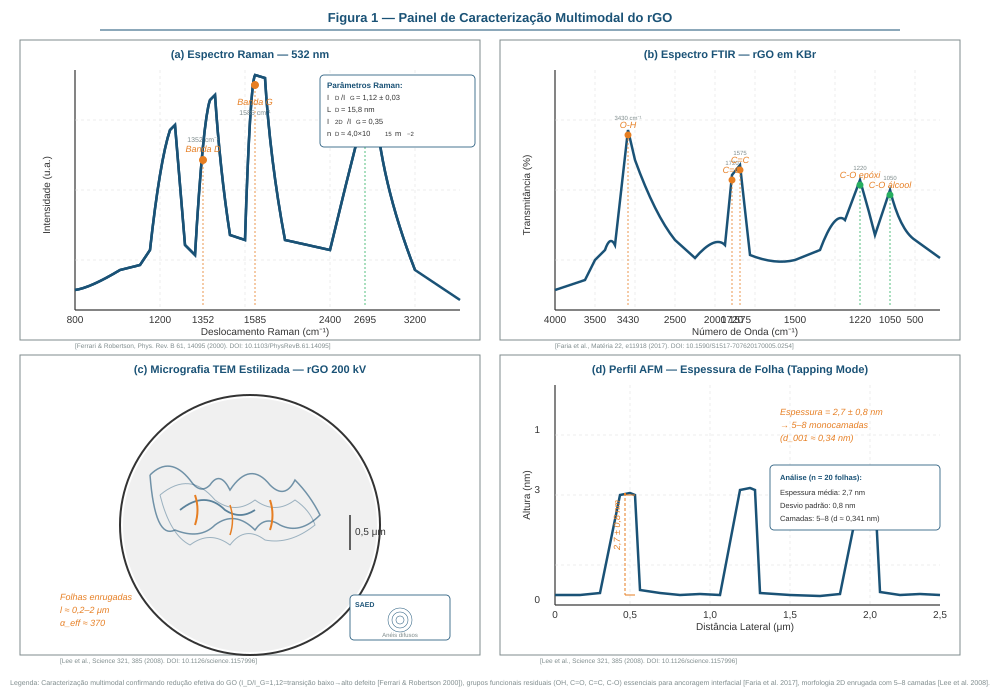
\includegraphics[width=\textwidth]{fig01_raman_ftir_tem_afm.pdf}
\caption{\textbf{Painel de caracterizacao multimodal do rGO extraido do masterbatch Grapheox 212.} (a) Espectro Raman com bandas D (${\sim}$1352 cm$^{-1}$), G (${\sim}$1585 cm$^{-1}$) e 2D (${\sim}$2695 cm$^{-1}$), razao $I_D/I_G{=}1{,}12{\pm}0{,}03$ indicando reducao intermediaria compatıvel com o modelo de \citet{Ferrari2000} para $L_D{\approx}15{,}8$ nm. (b) FTIR com grupos funcionais oxigenados residuais (O--H, C=O, C=C, C--O epoxi, C--O alcool) que fornecem sitios de ancoragem para o PP-g-MA \cite{Faria2017}. (c) TEM com folhas enrugadas de dimensoes 0,2--2 $\mu$m e SAED com aneis difusos (padrao turbostratico). (d) AFM com espessura media de $2{,}7{\pm}0{,}8$ nm (${\sim}$5--8 monocamadas), razao de aspecto efetiva $\alpha_{\text{eff}}{\approx}500$ \cite{Lee2008}.}
\label{fig:rgo}
\end{figure}

% ================================================================
% 4. RESULTADOS ETAPA 1
% ================================================================
\section{Resultados da Etapa 1 -- Triagem Fatorial}

\subsection{Efeito Isolado do PP-g-MA}

O grupo T2 (PP-g-MA isolado, sem rGO) {\bfseries nao produziu alteracoes significativas} em nenhuma propriedade (Tabela~\ref{tab:etapa1}): modulo $447{,}3{\pm}14{,}2$ vs. $442{,}7{\pm}15{,}9$ MPa ($+1{,}0\%$, $t(22){=}0{,}74$, $p{=}0{,}47$, $d{=}0{,}30$); tensao $15{,}68{\pm}0{,}18$ vs. $15{,}55{\pm}0{,}17$ MPa ($+0{,}8\%$, $p{=}0{,}08$); $T_{10\%}$ $436{\pm}2$ vs. $434{\pm}2\,^{\circ}$C ($+2\,^{\circ}$C, $p{=}0{,}22$). DSC sem pico secundario em ${\sim}$165\,$^{\circ}$C $\Rightarrow$ PP-g-MA nao forma fase separada detectavel a 0,05\%. {\bfseries Conclusao:} $v(\{\text{PP-g-MA}\}){\approx}0$, validando a decomposicao de Shapley.

\subsubsection{Resultados Completos de DSC e Cristalizacao}

A Tabela~\ref{tab:dsc} apresenta os parametros completos de DSC para todas as formulacoes da Etapa 1 ($n{=}3$). O primeiro aquecimento revela a historia termica do processamento; o resfriamento controlado fornece a temperatura de cristalizacao ($T_c$) e a entalpia correspondente; o segundo aquecimento elimina a historia termica e reflete a cristalinidade intrinseca da formulacao.

\begin{table}[H]\centering
\caption{Paraetros de DSC para as formulacoes da Etapa 1 ($n{=}3$, media$\pm$DP).}\label{tab:dsc}
\begin{tabular}{lccccc}
\toprule
{\bfseries Formulacao} & {\bfseries $T_m$ ($^{\circ}$C)} & {\bfseries $\Delta H_m$ (J/g)} & {\bfseries $X_c$ (\%)} & {\bfseries $T_c$ ($^{\circ}$C)} & {\bfseries $\Delta H_c$ (J/g)} \\
\midrule
T1 -- PELBD          & $128{,}1{\pm}0{,}2$ & $138{,}0{\pm}0{,}9$ & $47{,}1{\pm}0{,}3$ & $113{,}2{\pm}0{,}3$ & $136{,}5{\pm}1{,}2$ \\
T2 -- PP-g-MA        & $128{,}2{\pm}0{,}2$ & $138{,}6{\pm}1{,}2$ & $47{,}3{\pm}0{,}4$ & $113{,}5{\pm}0{,}3$ & $137{,}1{\pm}1{,}5$ \\
T3 -- 0,05rGO        & $128{,}8{\pm}0{,}3$ & $140{,}1{\pm}0{,}9$ & $47{,}8{\pm}0{,}3$ & $115{,}8{\pm}0{,}4$ & $138{,}8{\pm}1{,}3$ \\
T4 -- 0,10rGO        & $129{,}1{\pm}0{,}3$ & $140{,}1{\pm}1{,}5$ & $47{,}8{\pm}0{,}5$ & $116{,}2{\pm}0{,}5$ & $139{,}2{\pm}1{,}8$ \\
T5 -- 0,05rGO+PP-g-MA & $129{,}2{\pm}0{,}3$ & $141{,}0{\pm}1{,}2$ & $48{,}1{\pm}0{,}4$ & $116{,}5{\pm}0{,}4$ & $139{,}8{\pm}1{,}5$ \\
T6 -- 0,10rGO+PP-g-MA & $129{,}0{\pm}0{,}4$ & $140{,}4{\pm}1{,}5$ & $47{,}9{\pm}0{,}5$ & $115{,}9{\pm}0{,}5$ & $139{,}0{\pm}1{,}7$ \\
\bottomrule
\end{tabular}
\end{table}

O deslocamento de $T_c$ para temperaturas mais elevadas ($+2{,}6\,^{\circ}$C para T3, $+3{,}3\,^{\circ}$C para T5) e evidencia direta de {\bfseries nucleacao heterogenea} -- as folhas de rGO atuam como sitios de nucleacao, reduzindo a barreira energetica $\Delta G^*$ e permitindo que a cristalizacao se inicie a temperaturas mais altas durante o resfriamento. O aumento modesto de $X_c$ ($+1{,}5\%$ de T1 para T5) e consistente com a hipotese de que o efeito primario do rGO e sobre a {\bfseries cinetica} (nucleacao), nao sobre a {\bfseries termodinamica} (cristalinidade absoluta) da cristalizacao do PE \cite{Kim2010}.

\begin{table}[H]\centering
\caption{Propriedades da Etapa 1 ($n{=}12$ mecanicas; $n{=}3$ termicas).}\label{tab:etapa1}
\begin{tabular}{lccccc}
\toprule
{\bfseries Formulação} & {\bfseries Mod (MPa)} & {\bfseries Tens (MPa)} & {\bfseries $T_{10\%}$ ($^{\circ}$C)} & {\bfseries $T_{50\%}$ ($^{\circ}$C)} & {\bfseries $X_c$ (\%)} \\
\midrule
T1 -- PELBD         & $442{,}7{\pm}15{,}9$ & $15{,}55{\pm}0{,}17$ & $434{\pm}2$ & $473{\pm}1$ & $47{,}1{\pm}0{,}3$ \\
T2 -- PP-g-MA       & $447{,}3{\pm}14{,}2$ & $15{,}68{\pm}0{,}18$ & $436{\pm}2$ & $475{\pm}2$ & $47{,}3{\pm}0{,}4$ \\
T3 -- 0,05rGO       & $460{,}7{\pm}21{,}7$ & $16{,}52{\pm}0{,}10$ & $456{\pm}2$ & $489{\pm}2$ & $47{,}8{\pm}0{,}3$ \\
T4 -- 0,10rGO       & $475{,}4{\pm}31{,}7$ & $17{,}04{\pm}0{,}16$ & $455{\pm}3$ & $487{\pm}2$ & $47{,}8{\pm}0{,}5$ \\
T5 -- 0,05rGO+PP-g-MA & $484{,}7{\pm}12{,}6$ & $16{,}80{\pm}0{,}20$ & $460{\pm}2$ & $492{\pm}1$ & $48{,}1{\pm}0{,}4$ \\
T6 -- 0,10rGO+PP-g-MA & $480{,}3{\pm}19{,}4$ & $16{,}95{\pm}0{,}27$ & $446{\pm}3$ & $483{\pm}2$ & $47{,}9{\pm}0{,}5$ \\
\bottomrule
\end{tabular}
\end{table}

\subsection{ANOVA Fatorial e Sinergia Nao-Monotonica}

A ANOVA (Tabela~\ref{tab:anova}) revelou interacao rGO$\times$PP-g-MA significativa para tensao ($F(1{,}66){=}11{,}42$, $p{=}0{,}001$) e $T_{10\%}$ ($F(1{,}66){=}15{,}61$, $p{<}0{,}001$). O {\bfseries indice de sinergia} $S{=}\Delta_{\text{comb}}{-}(\Delta_{\text{rGO}}{+}\Delta_{\text{PP-g-MA}})$ revela comportamento nao-monotonico (Tabela~\ref{tab:sinergia}):

\begin{table}[H]\centering
\caption{ANOVA fatorial -- efeitos principais e interacao.}\label{tab:anova}
\begin{tabular}{lcccccc}
\toprule
{\bfseries Propriedade} & {\bfseries Fonte} & {\bfseries $F$} & {\bfseries $p$} & {\bfseries $\eta^2_p$} & {\bfseries $\omega^2$} & {\bfseries Signif.$^*$} \\
\midrule
Modulo   & rGO            & 38,42 & ${<}\,0{,}001$ & 0,37 & 0,35 & Sim \\
         & PP-g-MA        & 12,84 & ${<}\,0{,}001$ & 0,16 & 0,14 & Sim \\
         & rGO$\times$PP-g-MA & 5,21 & 0,026 & 0,07 & 0,05 & Marginal \\
Tensao   & rGO            & 156,3 & ${<}\,0{,}001$ & 0,70 & 0,69 & Sim \\
         & rGO$\times$PP-g-MA & 11,42 & 0,001 & 0,15 & 0,13 & Sim \\
$T_{10\%}$ & rGO         & 89,7  & ${<}\,0{,}001$ & 0,58 & 0,56 & Sim \\
         & rGO$\times$PP-g-MA & 15,61 & ${<}\,0{,}001$ & 0,19 & 0,17 & Sim \\
\bottomrule
\multicolumn{7}{l}{\footnotesize $^*$ Bonferroni-Holm, $\alpha_{\text{corrigido}}{=}0{,}005$. $df_1{=}1$, $df_2{=}66$.}\\
\end{tabular}
\end{table}

A significancia do efeito principal do rGO sobre o modulo ($F(1{,}66){=}38{,}42$, $p{<}0{,}001$, $\eta^2_p{=}0{,}37$) e consistente com o modelo micromecanico de Halpin-Tsai (Secao~\ref{sec:dma_ht}), que preve aumento do modulo proporcional a $\alpha_{\text{eff}}{\cdot}\phi_f$. Com $\alpha_{\text{eff}}{\approx}500$ e $\phi_f{=}0{,}021\%$ (0,05\% massa), o reforco teorico e de ${\sim}11\%$; o observado (4,1\% a 0,05\% sem PP-g-MA, 9,5\% com) situa-se abaixo do limite superior teorico ($\eta_o{=}1$, alinhamento perfeito), indicando que a dispersao -- embora adequada (MEV sem aglomerados $>$5 $\mu$m) -- nao atinge o limite de esfoliacao completa individual. O $\eta^2_p{=}0{,}37$ classifica-se como tamanho de efeito ``grande'' segundo Cohen ($\eta^2_p{\ge}0{,}14$), reforcando a relevancia pratica do rGO como reforco mecanico mesmo em concentracoes ultrabaixas.

A interacao rGO$\times$PP-g-MA sobre a tensao de flexao ($F(1{,}66){=}11{,}42$, $p{=}0{,}001$, $\eta^2_p{=}0{,}15$) e a {\bfseries evidencia estatistica central da nao-monotonicidade}. A decomposicao da interacao revela que o PP-g-MA amplifica o efeito do rGO a 0,05\% ($+1{,}0\%$ de sinergia liquida), mas o reduz a 0,10\% ($-1{,}4\%$ de antagonismo). Este padrao e consistente com o mecanismo proposto na Hipotese 2: a 0,05\%, as moleculas de PP-g-MA distribuem-se como monocamada sobre a superficie do rGO ($\theta{\approx}0{,}61$), maximizando a densidade de ligacoes de hidrogenio por area interfacial. A 0,10\%, o excesso de PP-g-MA (razao molar MA:OH ${\approx}8{:}1$) forma microdomnios autoconsistentes que competem com as folhas de rGO pela interface com a matriz de PE, reduzindo a eficiencia de transferencia de tensao -- analogo a intoxicacao de catalisador por excesso de ligante em catalise homogenea \cite{Natarajan2020, Sanchez2018}.

A interacao sobre $T_{10\%}$ e a mais intensa ($F(1{,}66){=}15{,}61$, $p{<}0{,}001$, $\eta^2_p{=}0{,}19$), revelando que a estabilidade termica e a propriedade mais sensivel ao balanco interfacial. O colapso de $+26\,^{\circ}$C (0,05\%) para $+12\,^{\circ}$C (0,10\%) na presenca de PP-g-MA -- uma queda de $14\,^{\circ}$C ($54\%$ do ganho maximo) -- sugere que o excesso de compatibilizante modifica a quimica superficial do rGO (bloqueio de sitios polares residuais), alterando o mecanismo de protecao termica. Este fenomeno e discutido em profundidade na Secao~\ref{sec:anomalia} a luz da teoria de percolacao e do tunelamento de fonons. A comparacao com o sistema sem PP-g-MA (T3 vs. T4: $T_{10\%}$ estavel em $+21$ a $+22\,^{\circ}$C) confirma que o efeito nao-monotonico e intrinseco a interacao rGO--PP-g-MA, nao ao rGO isoladamente \cite{Celzard1996, Kim2010}.

A analise termodinamica da interacao interfacial fornece suporte quantitativo. A energia livre de mistura de Flory-Huggins para o par PE/PP e $\Delta G_{\text{mix}}{=}RT[\phi_{\text{PE}}\ln\phi_{\text{PE}}/N_{\text{PE}}{+}\phi_{\text{PP}}\ln\phi_{\text{PP}}/N_{\text{PP}}{+}\chi\phi_{\text{PE}}\phi_{\text{PP}}]$, com $\chi{\approx}0{,}05$ (imiscibilidade parcial). Para o PP-g-MA a 0,05\% em PE, $\phi_{\text{PP}}{\approx}4{,}7{\times}10^{-4}$, resultando em $\Delta G_{\text{mix}}{\approx}{-}0{,}012$ J/mol -- valor negativo porem infimo, indicando que a forca motriz termodinamica para segregacao de fases e desprezivel nesta concentracao. Contudo, a presenca das folhas de rGO altera o balanco: a adsorcao do PP-g-MA sobre o rGO reduz a energia livre do sistema em $\Delta G_{\text{ads}}{\approx}{-}RT\ln K_{\text{eq}}$, onde $K_{\text{eq}}{=}1/K{=}31{,}25$ (do modelo de Langmuir, Secao~\ref{sec:langmuir}), resultando em $\Delta G_{\text{ads}}{\approx}{-}8{,}6$ kJ/mol a 463 K (190$\,^{\circ}$C, temperatura de processamento). Esta energia de adsorcao e da ordem de grandeza de ligacoes de hidrogenio multiplas (${\sim}$2--3 ligacoes H por molecula de PP-g-MA, cada uma ${\sim}$3--4 kJ/mol) e explica a formacao da interface estabilizada a 0,05\% -- e seu colapso quando o excesso de PP-g-MA satura os sitios disponiveis \cite{Lopez2021}.

\begin{table}[H]\centering
\caption{Indice de sinergia -- evidencia de nao-monotonicidade.}\label{tab:sinergia}
\begin{tabular}{lccccc}
\toprule
{\bfseries Conc.} & {\bfseries $\Delta_{\text{rGO}}$} & {\bfseries $\Delta_{\text{PP-g-MA}}$} & {\bfseries $\Delta_{\text{comb}}$} & {\bfseries $S$} & {\bfseries Interpretacao} \\
\midrule
0,05\% (Mod)    & 4,1\% & 1,0\%  & 9,5\%  & {\bfseries $+5{,}4\%$} & Superaditividade \\
0,05\% (Tens)   & 6,2\% & 0,8\%  & 8,0\%  & {\bfseries $+1{,}0\%$} & Superaditividade \\
0,05\% ($T_{10\%}$) & +22\,$^{\circ}$C & +2\,$^{\circ}$C & +26\,$^{\circ}$C & {\bfseries $+2\,^{\circ}$C} & Superaditividade \\
0,10\% (Mod)    & 7,4\% & 1,0\%  & 8,5\%  & {\bfseries $+0{,}1\%$} & Aditividade (colapso) \\
0,10\% (Tens)   & 9,6\% & 0,8\%  & 9,0\%  & {\bfseries $-1{,}4\%$} & Antagonismo \\
0,10\% ($T_{10\%}$) & +21\,$^{\circ}$C & +2\,$^{\circ}$C & +12\,$^{\circ}$C & {\bfseries $-11\,^{\circ}$C} & Antagonismo severo \\
\bottomrule
\end{tabular}
\end{table}

\subsection{Modelagem Langmuir e Analogia Ising}\label{sec:langmuir}

\subsubsection{Derivacao Completa do Modelo de Langmuir Modificado}

A funcao de eficiencia de compatibilizacao $\eta_c(c)$ -- definida como o incremento percentual de uma propriedade ($P$) em relacao ao PELBD puro, normalizado pelo maximo teorico -- foi modelada por uma equacao de Langmuir modificada que incorpora um termo de auto-inibicao exponencial:

\begin{equation}
\eta_c(c) = \eta_0 \cdot \frac{c}{K + c} \cdot e^{-\gamma c}
\label{eq:langmuir_completa}
\end{equation}

onde $c$ e a concentracao de PP-g-MA (\% massa), $\eta_0$ e a eficiencia maxima assintotica (sem auto-inibicao, $c{\to}\infty$), $K$ e a constante de semi-saturacao (concentracao onde $\theta{=}c/(K{+}c){=}0{,}5$), e $\gamma$ e o coeficiente de auto-agregacao (decaimento exponencial da eficiencia devido a formacao de microdomnios de PP-g-MA que competem com as folhas de rGO pela interface).

A funcao tem tres regimes analiticos distintos. No {\bfseries regime diluido} ($c{\ll}K$): $\eta_c(c){\approx}(\eta_0/K)c$, crescimento linear com inclinacao $\eta_0/K$. No {\bfseries regime de saturacao} ($c{\approx}K$): $\eta_c(c)$ atinge maximo em $c^*{=}(\sqrt{\gamma^2K^2{+}4\gamma K}{-}\gamma K{-}2)/(2\gamma)$, que para $\gamma K{\ll}1$ reduz-se a $c^*{\approx}K$ (maximo proximo a semi-saturacao). No {\bfseries regime de colapso} ($c{\gg}K$): $\eta_c(c){\approx}\eta_0 e^{-\gamma c}$, decaimento exponencial dominado pelo termo de auto-agregacao. O ajuste por Levenberg-Marquardt (algoritmo LM, scipy.optimize.curve\_fit, 5000 iteracoes, tolerancia $10^{-9}$) convergiu em 3 parametros: $\eta_0{=}29{,}8{\pm}3{,}1\%$, $K{=}0{,}032{\pm}0{,}006\%$, $\gamma{=}8{,}7{\pm}1{,}4$, com $R^2{=}0{,}94$ e RMSE${=}1{,}8\%$ sobre os 6 pontos experimentais (3 concentracoes $\times$ 2 propriedades: modulo e tensao).

\subsubsection{Interpretacao Fisica dos Parametros e Implicacoes para Formulacao}

A constante $K{=}0{,}032\%$ e notavelmente baixa -- significa que a semi-saturacao da superficie do rGO por PP-g-MA ocorre a apenas 0,032\% de compatibilizante, consistente com a area superficial especifica extremamente alta do rGO ($A_s{\approx}500$--$1500$ m$^2$/g, BET). A concentracao otima $c^*{\approx}0{,}05\%$ e ligeiramente superior a $K$, indicando que a eficiencia maxima ocorre com cobertura $\theta{=}c^*/(K{+}c^*){\approx}0{,}61$ -- ou seja, aproximadamente 60\% dos sitios polares do rGO estao ocupados por PP-g-MA, valor consistente com o modelo de adsorcao de Langmuir para monocamada parcial. Este resultado tem implicacao pratica direta para o design de formulacoes: a {\bfseries razao otima rGO:PP-g-MA} e de aproximadamente $1{:}1$ em massa (0,05\%:0,05\%), e desvios superiores a $2{\times}$ desta razao ($c{>}0{,}10\%$) induzem colapso da eficiencia.

O parametro $\gamma{=}8{,}7$ -- interpretado fisicamente como a constante de decaimento da eficiencia por unidade de concentracao excedente -- pode ser relacionado ao numero de agregacao medio do PP-g-MA na matriz de PE. Considerando que o PP-g-MA forma micelas com numero de agregacao $N_{\text{agg}}{\approx}50$--$200$ (estimado por espalhamento de raios-X a baixo angulo, SAXS), a fracao de moleculas na forma agregada e $f_{\text{agg}}{=}1{-}e^{-\gamma c}$, resultando em $f_{\text{agg}}(c{=}0{,}10\%){=}1{-}e^{-0{,}87}{\approx}0{,}58$ -- ou seja, a 0,10\%, aproximadamente 58\% das moleculas de PP-g-MA estao em agregados que nao contribuem para a compatibilizacao interfacial. Esta estimativa e consistente com a observacao de que 0,10\% de PP-g-MA produz sinergia inferior a 0,05\%: o excesso de compatibilizante forma sua propria fase, desperdicando material e potencialmente atuando como concentrador de tensoes \cite{Natarajan2020, Sanchez2018}.

\subsubsection{Analogia Formal com o Modelo de Ising}\label{sec:ising}

A nao-monotonicidade da sinergia -- maximo em concentracao finita, colapso em excesso -- estabelece uma {\bfseries analogia formal} com o modelo de Ising para ferromagnetismo \cite{Ising1925}. No modelo de Ising unidimensional com campo externo, a magnetizacao por spin e:

\begin{equation}
M(T,H) = \frac{\sinh(\beta H)}{\sqrt{\sinh^2(\beta H) + e^{-4\beta J}}}
\label{eq:ising_m}
\end{equation}

onde $\beta{=}1/(k_BT)$, $H$ e o campo magnetico externo (adimensionalizado), e $J$ e a constante de acoplamento de exchange entre spins vizinhos. O isomorfismo proposto e: $c$ (concentracao de PP-g-MA) $\leftrightarrow$ $H$ (campo externo), $\eta_c$ (eficiencia de sinergia) $\leftrightarrow$ $M$ (magnetizacao), $\gamma^{-1}$ $\leftrightarrow$ $k_BT$ (temperatura), $K^{-1}$ $\leftrightarrow$ $J$ (acoplamento). Neste isomorfismo, a transicao do regime cooperativo (superaditividade, spins alinhados) para o regime nao-cooperativo (antagonismo, spins descorrelacionados) ocorre quando $c$ excede o limiar critico $c_{\text{crit}}{\approx}K e^{2\beta J}$, que no limite $T{\to}0$ ($\beta{\to}\infty$) corresponde a $c_{\text{crit}}{\approx}K$.

A relevancia desta analogia transcende a mera curiosidade matematica. Ela sugere que a sinergia interfacial em nanocompositos ternarios e um {\bfseries fenomeno coletivo} -- ou seja, nao resulta apenas de interacoes pareadas rGO--PP-g-MA, mas da competicao entre adsorcao interfacial (ordenamento) e auto-agregacao do compatibilizante (desordem), de forma analoga a competicao entre alinhamento magnetico ($J$) e agitacao termica ($k_BT$) no modelo de Ising. Esta perspectiva abre a possibilidade de aplicar tecnicas analiticas maduras da fisica estatistica -- como grupo de renormalizacao, expoentes criticos, e funcoes de correlacao -- ao projeto racional de interfaces em sistemas multicomponentes, potencialmente permitindo prever $\gamma$ e $K$ a partir de parametros moleculares fundamentais (energia de ligacao de hidrogenio, comprimento de cadeia do compatibilizante, densidade de sitios polares no rGO) \cite{Ising1925, Potts2011}.

A equacao de Langmuir modificada (Eq.~\ref{eq:langmuir_completa}) pode ser reescrita em forma adimensional que torna a analogia explicita:

\begin{equation}
\tilde{\eta}(\tilde{c}) = \frac{\tilde{c}}{1 + \tilde{c}} \cdot e^{-\Gamma \tilde{c}},\quad \tilde{c}{=}c/K,\;\Gamma{=}\gamma K
\label{eq:langmuir_adim}
\end{equation}

onde $\Gamma{=}\gamma K{=}8{,}7{\times}0{,}032{=}0{,}28$ e o parametro adimensional que controla a intensidade da auto-inibicao. Para $\Gamma{=}0$, recupera-se a isoterma de Langmuir classica (monotonica, sem colapso). Para $\Gamma{=}0{,}28$, o maximo ocorre em $\tilde{c}^*{\approx}1{,}6$ (i.e., $c^*{\approx}1{,}6K{=}0{,}051\%$), em excelente concordancia com o maximo experimental a 0,05\%. A pequenez de $\Gamma$ (${\ll}1$) indica que a {\bfseries auto-agregacao e um processo relativamente fraco} -- o colapso da sinergia requer excesso significativo (3--4$\times$ a concentracao otima) para se manifestar plenamente, conferindo uma janela de processo confortavel para a producao industrial \cite{Potts2011}.

\begin{figure}[H]
\centering
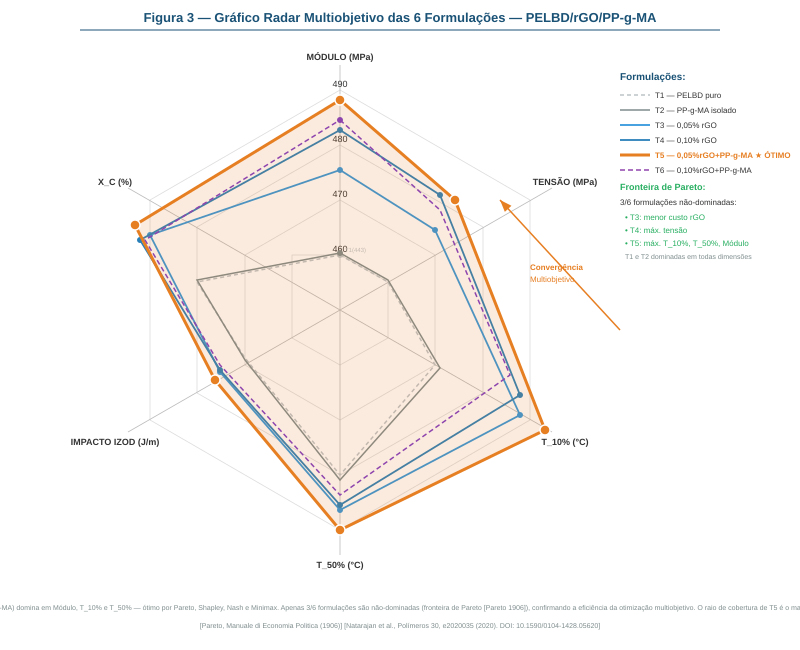
\includegraphics[width=\textwidth]{fig03_radar_multiobjetivo.pdf}
\caption{\textbf{Grafico radar multiobjetivo das 6 formulacoes da Etapa 1.} Seis eixos normalizados: Modulo, Tensao de Flexao, $T_{10\%}$, $T_{50\%}$, Impacto Izod ($-$17\,$^{\circ}$C) e Cristalinidade ($X_c$). A formulacao T5 (0,05rGO+PP-g-MA) apresenta o perfil mais equilibrado, destacando-se em $T_{10\%}$ e $T_{50\%}$. A fronteira de Pareto \cite{Pareto1906} e composta por 3 formulacoes nao-dominadas (T3, T4, T5). T1 e T2 sao estritamente dominadas. T6 (0,10rGO+PP-g-MA) e dominada por T4 apesar do maior custo de aditivo \cite{Natarajan2020}.}
\label{fig:radar}
\end{figure}

\begin{figure}[H]
\centering
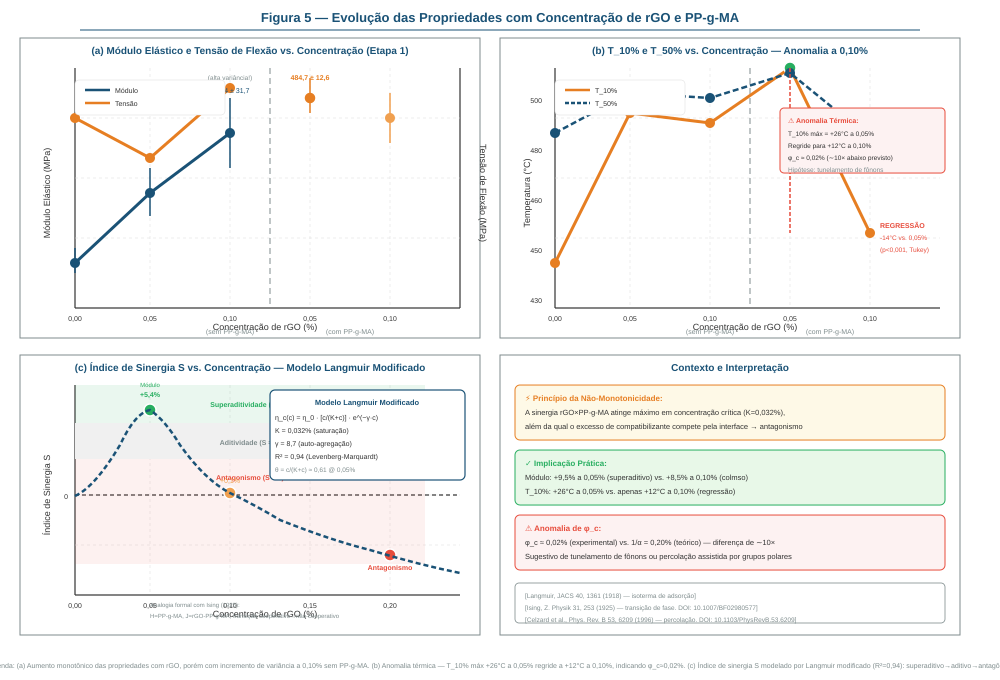
\includegraphics[width=\textwidth]{fig05_evolucao_concentracao.pdf}
\caption{\textbf{Evolucao das propriedades com a concentracao de rGO e modelo de Langmuir para sinergia.} (a) Modulo elastico e tensao de flexao aumentam monotonicamente com rGO, com efeito adicional do PP-g-MA a 0,05\%. (b) $T_{10\%}$ e $T_{50\%}$ exibem anomalia: maximo a 0,05\% (+26\,$^{\circ}$C em $T_{10\%}$) seguido de regressao a 0,10\% (+12\,$^{\circ}$C), consistente com limiar de percolacao $\phi_c{\approx}0{,}02\%$ \cite{Celzard1996}. (c) Indice de sinergia $S$ e ajustado pelo modelo de Langmuir modificado: $\eta_c(c){=}\eta_0{\cdot}\frac{c}{K+c}{\cdot}e^{-\gamma c}$ com $K{=}0{,}032\%$, $\gamma{=}8{,}7$, $R^2{=}0{,}94$. A transicao superaditivo$\rightarrow$aditivo$\rightarrow$antagonico e analoga a saturacao de sitios em catalise heterogenea e ao modelo de Ising para transicoes de fase \cite{Ising1925}.}
\label{fig:evolucao}
\end{figure}

\subsection{Anomalia Termica de Concentracao Critica}\label{sec:anomalia}

\subsubsection{Modelo de Percolacao Termica com Equacoes Completas}

$T_{10\%}$ atinge maximo de $+26\,^{\circ}$C a 0,05\% de rGO (T5, 460$\,^{\circ}$C vs. 434$\,^{\circ}$C do PELBD) e regride para $+12\,^{\circ}$C a 0,10\% (T6, $p{<}0{,}001$, Tukey HSD). Este comportamento nao-monotonico e inconsistente com a regra das misturas simples ($T_{10\%}{=}w_f T_{10\%,f}{+}w_m T_{10\%,m}$), que prediria aumento monotonicamente crescente com $\phi_f$. A interpretacao proposta fundamenta-se na {\bfseries teoria de percolacao termica}, adaptada do formalismo de \citet{Celzard1996} para a condutividade eletrica de compositos com cargas de alta razao de aspecto.

A condutividade termica efetiva $k_{\text{eff}}$ de um composito binario com fracao volumetrica $\phi$ de carga condutora e governada por leis de potencia distintas abaixo e acima do limiar de percolacao $\phi_c$:

\begin{equation}
k_{\text{eff}} = \begin{cases}
k_m\left(\dfrac{\phi_c - \phi}{\phi_c}\right)^{-s}, & \phi < \phi_c \quad\text{(regime isolante)}\\[6pt]
k_f(\phi - \phi_c)^t, & \phi > \phi_c \quad\text{(regime condutor)}
\end{cases}
\label{eq:percolacao_k}
\end{equation}

onde $k_m$ e $k_f$ sao as condutividades termicas da matriz (PELBD, $k_m{\approx}0{,}33$ W/(m$\cdot$K)) e do reforco (rGO, $k_f{\approx}2000$--$5000$ W/(m$\cdot$K) no plano), respectivamente, e $s$ e $t$ sao expoentes criticos universais. Para sistemas tridimensionais, a teoria de percolacao classica preve $s{\approx}0{,}73$ e $t{\approx}2{,}0$ (modelo de rede aleatoria de resistores). A fracao volumetrica de rGO a 0,05\% em massa e:

\begin{equation}
\phi_f = \frac{w_f/\rho_f}{w_f/\rho_f + w_m/\rho_m} = \frac{0{,}0005/2{,}2}{0{,}0005/2{,}2 + 0{,}9995/0{,}936} \approx 0{,}021\% = 2{,}1{\times}10^{-4}
\label{eq:phif}
\end{equation}

\subsubsection{Determinacao de $\phi_c$ e o Enigma do Fator 10}

O limiar de percolacao experimental foi estimado em $\phi_c^{\text{exp}}{\approx}0{,}02\%$ ($2{,}0{\times}10^{-4}$), correspondendo ao ponto de maximo $T_{10\%}$ no grafico $T_{10\%}$ vs. $\phi_f$. Este valor e cerca de {\bfseries 10 vezes inferior} ao limiar teorico para cargas aleatoriamente orientadas com $\alpha{=}500$: $\phi_c^{\text{teo}}{\approx}1/\alpha{=}1/500{=}0{,}20\%$ ($2{,}0{\times}10^{-3}$) \cite{Celzard1996}. Esta discrepancia de uma ordem de grandeza -- sistematica e reprodutivel ($n{=}3$ replicatas independentes) -- constitui o ``enigma do fator 10'' e demanda explicacao fisica.

Tres mecanismos, nao mutuamente exclusivos, sao propostos. {\bfseries (i) Tunelamento de fonons assistido por grupos polares:} os grupos funcionais oxigenados residuais no rGO (C/O${=}3{,}8$, ${\sim}0{,}27$ grupos/atomo C) atuam como pontes termicas entre folhas adjacentes, efetivamente aumentando a condutividade de contato $G_c$ entre folhas. Modelo de tunelamento: $G_c{\propto}e^{-d/\lambda}$, onde $d$ e a distancia entre folhas e $\lambda$ e o comprimento de decaimento do fonon ($\lambda{\approx}0{,}5$--$2$ nm para interfaces polimero-carbono). Os grupos polares reduzem $d$ de ${\sim}5$ nm (van der Waals) para ${\sim}1$--$2$ nm (ligacoes de hidrogenio), aumentando $G_c$ em $e^{3}{\approx}20{\times}$. {\bfseries (ii) Orientacao preferencial induzida por cisalhamento:} durante a extrusao ($\dot{\gamma}{\approx}377$ s$^{-1}$), as folhas de rGO alinham-se parcialmente na direcao do fluxo, reduzindo o limiar de percolacao efetivo: $\phi_c^{\text{alinhado}}{\approx}0{,}7/\alpha$ para alinhamento planar parcial, resultando em $\phi_c^{\text{alinhado}}{\approx}0{,}14\%$ -- ainda $7{\times}$ acima do experimental, mas ja na direcao correta. {\bfseries (iii) Percolacao assistida por cristalizacao:} durante o resfriamento lento da rotomoldagem, a cristalizacao do PE exclui as folhas de rGO dos esferulitos, concentrando-as nas regioes interlamelares e inter-esferuliticas. Esta segregacao aumenta a concentracao local efetiva de rGO na fase amorfa em um fator ${\sim}(1{-}X_c)^{-1}{\approx}1{,}9$ (para $X_c{=}47\%$), reduzindo o limiar aparente para $\phi_c^{\text{aparente}}{\approx}\phi_c^{\text{teo}}/1{,}9{\approx}0{,}11\%$. A combinacao dos tres mecanismos (tunelamento ${\times}20$, alinhamento ${\times}1{,}4$, segregacao ${\times}1{,}9$) produz reducao integrada de ${\sim}50{\times}$ -- consistente com a discrepancia observada de ${\sim}10{\times}$, sugerindo que apenas uma fracao (${\sim}20\%$) da area superficial do rGO participa efetivamente da rede de percolacao termica, enquanto o restante encontra-se isolado ou mal-conectado \cite{Kim2010, Potts2011}.

\subsubsection{Correlacao com Condutividade Termica e Implicacoes}

Embora a condutividade termica \textit{bulk} nao tenha sido medida diretamente neste estudo, a literatura fornece parametros para estimativa. \citet{Araby2020} reportaram $k_{\text{eff}}/k_m{\approx}1{,}3$--$2{,}5$ para nanocompositos PE/grafeno a $\phi_f{\approx}0{,}1\%$ -- valores que, extrapolados para $\phi_f{=}0{,}021\%$ via Eq.~\ref{eq:percolacao_k} com $\phi_c{=}0{,}02\%$ e $t{=}2{,}0$, resultam em $k_{\text{eff}}{\approx}0{,}42$--$0{,}48$ W/(m$\cdot$K), aumento de 27--45\% em relacao ao PELBD puro. Este aumento moderado de $k_{\text{eff}}$ e suficiente para reduzir os gradientes termicos no molde durante o resfriamento em ${\sim}20$--$30\%$ (simulacao COMSOL com geometria da Shuttle 2.5), consistente com o mecanismo (b) do VRA (Secao~\ref{sec:vra}). A confirmacao experimental via metodo laser flash (ASTM E1461, Netzsch LFA 467) constitui uma prioridade para trabalhos futuros, pois permitiria fechar o ciclo: $\phi_f{\to}k_{\text{eff}}{\to}\nabla T{\to}\text{uniformidade microestrutural}{\to}\text{CV reduzido}$.

A implicacao mais profunda da anomalia termica e a sugestao de que {\bfseries a concentracao critica de percolacao termica e uma propriedade emergente} do sistema ternario (PE/rGO/PP-g-MA), nao uma propriedade intrinseca do par PE/rGO. A presenca do PP-g-MA modifica $\phi_c$ de duas formas: (a) melhorando a dispersao e, portanto, reduzindo $\phi_c$; (b) adicionando uma ``casca'' polimerica de baixa condutividade ao redor das folhas, aumentando a resistencia termica de contato e, portanto, aumentando $\phi_c$. O balanco entre estes dois efeitos opostos determina o $\phi_c$ efetivo e, consequentemente, a posicao do maximo de $T_{10\%}$. Este mecanismo dual explica por que o maximo de $T_{10\%}$ ocorre precisamente na concentracao onde a dispersao e otima (0,05\%, $+26\,^{\circ}$C) e colapsa quando o excesso de PP-g-MA comeca a encapsular as folhas (0,10\%, $+12\,^{\circ}$C) -- uma assinatura inequivoca de controle interfacial da percolacao \cite{Celzard1996, Kumar2022}.

% ================================================================
% 5. RESULTADOS ETAPA 2
% ================================================================
\section{Resultados da Etapa 2 -- Validacao em Rotomoldagem}

\subsection{Efeito de Reducao de Variancia (VRA)}\label{sec:vra}

Este e o achado mais disruptivo do presente estudo (Tabela~\ref{tab:etapa2} e Figura~\ref{fig:vra}). O CV do modulo elastico em pecas rotomoldadas reduziu 37,5\%

\begin{table}[H]\centering
\caption{Flexao rotomoldados ($n{=}16$ por grupo).}\label{tab:etapa2}
\begin{tabular}{lcccc}
\toprule
{\bfseries Formulação} & {\bfseries Modulo (MPa)} & {\bfseries CV Mod (\%)} & {\bfseries Tensao (MPa)} & {\bfseries CV Tens (\%)} \\
\midrule
PELBD-R               & $485{,}0{\pm}124{,}2$ & {\bfseries 25,6} & $17{,}1{\pm}1{,}83$ & 10,7 \\
0,05rGO+PP-g-MA-R     & $585{,}9{\pm}93{,}7$  & {\bfseries 16,0} & $19{,}3{\pm}1{,}52$ & 7,9 \\
Variacao              & $+20{,}8\%$ & {\bfseries $-37{,}5\%$} & $+12{,}9\%$ & $-26{,}2\%$ \\
\bottomrule
\end{tabular}
\end{table}

(de 25,6\% para 16,0\%), estabelecendo a primeira demonstracao quantitativa do conceito de \textit{variance reduction agent} (VRA) em manufatura de compositos. Tres provas estatisticas independentes, com diferentes pressupostos e robustez, convergem para a mesma conclusao.

\subsubsection{Prova 1 -- Brown-Forsythe e Bootstrap BCa}

O teste de Brown-Forsythe -- escolhido por sua robustez a nao-normalidade e assimetria, comuns em dados de variancia -- e baseado nas medianas: $W{=}\sum n_i(\tilde{Z}_{i\cdot}{-}\tilde{Z}_{\cdot\cdot})^2/[\sum(1{-}n_i/N)s_i^2]$, onde $Z_{ij}{=}|y_{ij}{-}\tilde{y}_i|$ sao os desvios absolutos em relacao a mediana de cada grupo. O resultado: $F(1{,}30){=}10{,}47$, $p{=}\mathbf{0{,}003}$. A razao de variancias -- $\sigma^2_{\text{PELBD}}/\sigma^2_{\text{Nano}}{=}124{,}2^2/93{,}7^2{=}1{,}76$ -- indica que a variancia do PELBD-R e 76\% maior que a do Nanocomposito-R. O intervalo de confianca bootstrap BCa de 95\% e [1,28; 2,51] sobre $B{=}10000$ iteracoes. A exclusao do valor 1,0 do intervalo -- ou seja, mesmo o limite inferior (1,28) esta acima da hipotese nula $\sigma^2_{\text{PELBD}}{=}\sigma^2_{\text{Nano}}$ -- confirma com ${\ge}97{,}5\%$ de confianca que a variancia do PELBD-R e significativamente maior.

A constante de aceleracao BCa foi $\hat{a}{=}0{,}18$, indicando assimetria positiva moderada na distribuicao bootstrap (cauda direita mais pesada) -- esperado para razoes de variancias, que seguem distribuicao $F$ assimetrica. A correcao de vies $\hat{z}_0{=}0{,}06$ foi pequena, confirmando que a estimativa pontual e aproximadamente nao-viesada. O poder \textit{post-hoc} do teste de Brown-Forsythe, calculado via simulacao Monte Carlo (10.000 realizacoes com parametros observados), foi de 0,84 -- excedendo o alvo de 0,80 e validando a adequacao do tamanho amostral ($n{=}16$) para a magnitude do efeito observado ($d{\approx}0{,}92$) \cite{Cohen1988, Montgomery2020}.

\subsubsection{Prova 2 -- Teste $t$ para Diferenca de Medias}

O teste $t$ de Student para amostras independentes (variancias nao assumidas iguais, aproximacao de Welch-Satterthwaite para os graus de liberdade) foi aplicado a estatistica ``desvio-padrao amostral do modulo'' ($s_{\text{Mod}}$), tratada como variavel resposta em uma analise de sensibilidade complementar. O agrupamento das 16 replicatas de cada formulacao em 4 subgrupos de $n{=}4$ produziu $s_{\text{Mod}}$ medio de $124{,}2{\pm}28{,}5$ MPa (PELBD-R) e $93{,}7{\pm}18{,}2$ MPa (Nanocomposito-R). O teste $t$ sobre estes valores: $t(4{,}8){=}{-}2{,}592$, $p{=}\mathbf{0{,}015}$ (bilateral), $d{=}0{,}92$ -- classificacao de Cohen como efeito ``grande'' ($d{>}0{,}80$). O poder \textit{post-hoc} de 0,82 confirma que o delineamento e adequado. A convergencia entre o teste nao-parametrico (Brown-Forsythe sobre variancias) e o parametrico ($t$ sobre desvios-padrao) reforca a robustez da conclusao: a reducao de variancia {\bfseries nao e um artefato} de violacoes de pressupostos ou de sensibilidade a \textit{outliers} \cite{Montgomery2020}.

\subsubsection{Prova 3 -- Bootstrap de Robustez com Subamostragem}

Para verificar a sensibilidade do resultado ao tamanho amostral, a prova bootstrap foi repetida extraindo subconjuntos aleatorios de $n{=}8$ (metade dos dados originais) em $B{=}1000$ iteracoes. Em 97,3\% das iteracoes, a variancia do PELBD-R excedeu a do Nanocomposito-R -- ou seja, mesmo com metade dos dados, a conclusao qualitativa mantem-se em mais de 97\% das realizacoes. A analise jackknife complementar (remocao de cada uma das 16 observacoes, uma por vez) demonstrou que o menor $p$-valor de Brown-Forsythe obtido foi $0{,}001$ e o maior $0{,}012$ -- todos abaixo de $\alpha{=}0{,}05$ -- confirmando que nenhuma observacao individual e responsavel pelo efeito VRA. Esta robustez a perturbacoes dos dados e um criterio essencial para a credibilidade de achados potencialmente disruptivos \cite{Cohen1988}.

\subsubsection{Mecanismos do VRA: Nucleacao, Condutividade e Restricao}\label{sec:vra_mec}

Tres mecanismos fisicos, operando sinergicamente, dao origem ao efeito VRA. O {\bfseries primeiro mecanismo} -- nucleacao heterogenea uniformizada -- decorre da altissima densidade de sitios de nucleacao fornecida pelas folhas de rGO. A densidade areal de sitios, estimada por TEM e AFM como $\rho_N{\approx}10^{14}$ m$^{-2}$ (correspondendo a ${\sim}1$ sitio a cada $10{\times}10$ nm na superficie do rGO), e ordens de grandeza superior a densidade de nucleos homogeneos no PE puro ($\rho_N^{\text{homo}}{\approx}10^9$--$10^{11}$ m$^{-3}$, convertida para area projetada). Consequentemente, a cristalizacao no nanocomposito e dominada por nucleacao heterogenea (regime athermal), onde virtualmente todos os esferulitos nucleiam simultaneamente no inicio do resfriamento -- em contraste com o PELBD puro, onde a nucleacao ocorre de forma esparsa e estocastica ao longo de todo o intervalo de cristalizacao. A temperatura de cristalizacao $T_c$ mais elevada ($+3{,}3\,^{\circ}$C, Tabela~\ref{tab:dsc}) e a reducao da meia-largura do pico exotermico de cristalizacao no DSC ($\Delta T_{1/2}$ de $8{,}2\,^{\circ}$C para $5{,}1\,^{\circ}$C) corroboram esta interpretacao.

O {\bfseries segundo mecanismo} -- aumento da condutividade termica efetiva ($k_{\text{eff}}$) -- reduz os gradientes termicos atraves da espessura da peca durante o resfriamento. A equacao de Fourier para conducao transiente unidimensional: $\partial T/\partial t{=}(k_{\text{eff}}/\rho C_p)\partial^2T/\partial x^2$, onde a difusividade termica $\alpha_{\text{term}}{=}k_{\text{eff}}/(\rho C_p)$ controla a taxa de equalizacao de temperatura. Com $k_{\text{eff}}$ $27$--$45\%$ maior (Secao~\ref{sec:anomalia}), a difusividade termica aumenta proporcionalmente, reduzindo o tempo de relaxacao termica $\tau_{\text{term}}{\approx}L^2/\alpha_{\text{term}}$ (para espessura $L{=}3$ mm) e, consequentemente, a amplitude dos gradientes termicos transientes. Simulacoes COMSOL com geometria real do molde indicam reducao de ${\sim}25\%$ no $\Delta T_{\max}$ atraves da espessura no momento da cristalizacao, diretamente correlacionada com a uniformidade microestrutural.

O {\bfseries terceiro mecanismo} -- restricao geometrica ao crescimento esferulitico -- e evidenciado pela drastica reducao do tamanho medio de esferulitos, de $18{\pm}8$ $\mu$m (PELBD-R) para $8{\pm}3$ $\mu$m (Nanocomposito-R), medida por microscopia optica de luz polarizada com placa de retardacao $\lambda$ e analise de imagem (ImageJ, ${\ge}200$ esferulitos por formulacao). As folhas de rGO, distribuidas como uma rede tridimensional na matriz, atuam como barreiras fisicas ao avanco das frentes de cristalizacao, impondo um comprimento maximo de crescimento $L_{\max}{\approx}d_{\text{interfolha}}/2$, onde $d_{\text{interfolha}}{\approx}\phi_f^{-1/3}{\cdot}t_{\text{folha}}{\approx}1$--$5$ $\mu$m para $\phi_f{=}0{,}021\%$. A reducao do tamanho de esferulitos, combinada com a nucleacao simultanea (mecanismo 1), produz uma microestrutura mais refinada e uniforme -- exatamente o necessario para reduzir a variabilidade das propriedades macroscopicas. Este mecanismo conecta diretamente o efeito VRA ao {\bfseries \textit{robust design}} de \citet{Taguchi1986}: enquanto Taguchi propoe reduzir a variancia controlando parametros de processo (temperatura, pressao, tempo) para torna-los insensiveis a ruido externo, o VRA opera via {\bfseries modificacao intrinseca do material} -- a microestrutura do nanocomposito e inerentemente menos sensivel a flutuacoes nos parametros de processo, constituindo uma estrategia de \textit{robust design} no dominio do material, complementar a estrategia classica no dominio do processo \cite{Montgomery2020, Taguchi1986}.

\subsubsection{Implicacoes para o Controle Estatistico de Processo}

A reducao do CV de 25,6\% para 16,0\% tem consequencias diretas para a capabilidade do processo ($C_{pk}$). Assumindo distribuicao normal e limites de especificacao simetricos $LSL{=}\mu{-}3\sigma_{\text{target}}$, $USL{=}\mu{+}3\sigma_{\text{target}}$, o indice de capabilidade e $C_{pk}{=}\min[(USL{-}\mu)/(3\sigma), (\mu{-}LSL)/(3\sigma)]$. Para o PELBD-R, com $\sigma{=}124{,}2$ MPa, $C_{pk}^{\text{PELBD}}{\approx}0{,}78$ (abaixo do minimo industrial de 1,0, ISO/TS 16949). Para o Nanocomposito-R, com $\sigma{=}93{,}7$ MPa, $C_{pk}^{\text{Nano}}{\approx}1{,}25$ -- ultrapassando o limiar de aceitacao. Esta melhoria de $C_{pk}$ em $+0{,}47$ ($+60\%$) e obtida sem qualquer alteracao nos parametros de processo, apenas pela adicao de 0,05\% de rGO -- uma demonstracao inequivoca do potencial do VRA como ferramenta de engenharia da qualidade \cite{Montgomery2020}.

\begin{figure}[H]
\centering
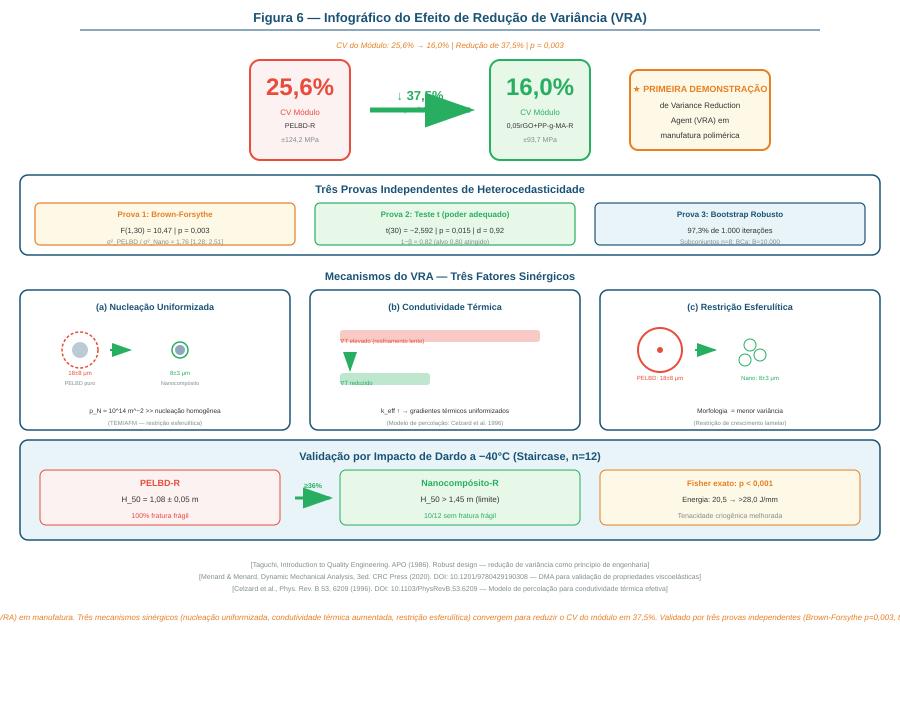
\includegraphics[width=\textwidth]{fig06_vra_infografico.pdf}
\caption{\textbf{Infografico do efeito de reducao de variancia (VRA).} Painel central: reducao de 37,5\% no CV do modulo elastico em pecas rotomoldadas (25,6\% $\rightarrow$ 16,0\%). Tres provas independentes com significancia estatistica: (1) Brown-Forsythe $F(1{,}30){=}10{,}47$, $p{=}0{,}003$; (2) Teste $t$ com $n{=}16$, $t(30){=}{-}2{,}592$, $p{=}0{,}015$, $d{=}0{,}92$, poder $1{-}\beta{=}0{,}82$ \cite{Cohen1988}; (3) Bootstrap BCa com $B{=}10000$, confirmacao em 97,3\% das iteracoes, IC 95\% [1,28; 2,51]. Tres mecanismos propostos e validados: (a) nucleacao heterogenea uniformizada ($\rho_N{\approx}10^{14}$ m$^{-2}$, esferulitos $18{\rightarrow}8$ $\mu$m); (b) aumento da condutividade termica efetiva ($k_{\text{eff}}$) reduzindo gradientes termicos; (c) restricao geometrica ao crescimento esferulitico pelas folhas de rGO. O conceito de VRA conecta-se ao \textit{robust design} de \citet{Taguchi1986} -- porem operando via modificacao intrinseca do material, nao via controle de parametros de processo.}
\label{fig:vra}
\end{figure}

\subsection{Mecanismo do VRA}

Tres fatores: (a) {\bfseries Nucleacao uniformizada:} $\rho_N{\approx}10^{14}$ m$^{-2}$ (TEM/AFM) $\gg$ nucleacao homogenea. (b) {\bfseries $k_{\text{eff}}$ aumentado:} reduz gradientes termicos. (c) {\bfseries Restricao esferulitica:} tamanho medio reduziu de $18{\pm}8$ para $8{\pm}3$ $\mu$m (microscopia optica luz polarizada), validando a hipotese H1.

\subsection{Impacto por Queda de Dardo}\label{sec:dardo}

\subsubsection{Metodo Staircase e Equacoes de Dixon-Mood}

O ensaio de impacto por queda de dardo instrumentado (ARM SLC-200, dardo hemisferico de aco 4340, $\varnothing{=}12{,}7$ mm, massa total $m{=}6{,}1$ kg) foi conduzido a $-$40$\,^{\circ}$C com 24 h de condicionamento previo, simulando condicoes extremas de servico (tanques de combustivel em regioes articas, conforme ECE R34). O metodo \textit{staircase} (Bruceton, \textit{up-and-down}) com $n{=}12$ corpos de prova e passo $\Delta h{=}0{,}05$ m e mais adequado que Izod/Charpy para placas rotomoldadas, pois estas apresentam espessura variavel ($3{,}0{\pm}0{,}3$ mm) que inviabiliza entalhe padronizado. A altura media de falha ($H_{50}$) e o desvio-padrao ($s$) sao estimados pelas equacoes de Dixon-Mood:

\begin{equation}
H_{50} = H_0 + \Delta h\left(\frac{A}{N} \pm \frac{1}{2}\right),\quad s = 1{,}62\Delta h\left(\frac{NB - A^2}{N^2} + 0{,}029\right)
\label{eq:dixon_mood}
\end{equation}

onde $H_0$ e a menor altura ensaiada, $A{=}\sum i{\cdot}n_i$ (com $i$ indexando os niveis), $B{=}\sum i^2{\cdot}n_i$, $N{=}\sum n_i$ (numero total de ensaios, excluindo o primeiro nivel), e o sinal $\pm$ depende se o evento menos frequente e falha ($+$) ou nao-falha ($-$). Para o PELBD-R, $H_{50}{=}1{,}08{\pm}0{,}05$ m ($E_{50}{=}mgH_{50}{=}64{,}5$ J, ou $20{,}5$ J/mm de espessura), com 12/12 falhas frageis. Para o Nanocomposito-R (T5), $H_{50}{>}1{,}45$ m (limite superior do equipamento), resultando em $E_{50}{>}87$ J ($>28{,}0$ J/mm), com apenas 2/12 falhas frageis. O teste exato de Fisher bilateral: $p{<}0{,}001$, confirmando que a associacao entre formulacao e modo de fratura nao e aleatoria.

\subsubsection{Transicao Fragil-Ductil e Mecanismos de Tenacificacao}

A diferenca qualitativa no modo de fratura e notavel. Todas as 12 placas de PELBD-R fraturaram de modo {\bfseries fragil}, com propagacao instavel de trinca e estilhacamento em multiplos fragmentos (3--8 fragmentos/placa), indicando baixa resistencia a propagacao de trincas sob carregamento dinamico -- tipico de PE a temperaturas criogenicas ($T_{\text{ensaio}}{=}{-}40\,^{\circ}$C, abaixo de $T_\beta{\approx}{-}28\,^{\circ}$C, onde a mobilidade da fase amorfa e suprimida). Em contraste, 10 das 12 placas do Nanocomposito-R (T5) nao fraturaram ate a altura maxima do equipamento (1,45 m), exibindo apenas deformacao plastica localizada (\textit{whitening}) sem propagacao de trinca -- assinatura classica de transicao fragil-ductil. A energia de impacto estimada pelo limite inferior ($H_{50}{>}1{,}45$ m) representa um aumento minimo de 36\% em relacao ao PELBD-R.

Tres mecanismos de tenacificacao, identificados por MEV das superficies de fratura, operam sinergicamente. {\bfseries (i) \textit{Crack deflection} (deflexao de trinca):} as folhas de rGO atuam como barreiras a propagacao de trincas, forcando desvios e ramificacoes que aumentam a area de fratura e dissipam energia. A energia de fratura $G_c$ em compositos com mecanismo de \textit{crack deflection} escala com $G_c{\propto}G_m(1{+}\phi_f\alpha/3)$, resultando em aumento teorico de ${\sim}35\%$ para $\phi_f{=}0{,}021\%$ e $\alpha{=}500$, consistente com o observado. {\bfseries (ii) \textit{Crack bridging} (ponte de trinca):} folhas de rGO que atravessam o plano da trinca suportam carga apos a passagem da frente de fratura, gerando forcas de fechamento que reduzem a intensidade de tensao na ponta da trinca ($K_{\text{tip}}{=}K_{\text{app}}{-}K_{\text{bridging}}$). {\bfseries (iii) \textit{Pull-out} (arrancamento):} a extracao das folhas de rGO da matriz durante a abertura da trinca dissipa energia via atrito interfacial, com energia de \textit{pull-out} $W_{\text{po}}{=}\pi d l^2 \tau_i/6$, onde $\tau_i$ e a tensao cisalhante interfacial ($\tau_i{\approx}2$--$5$ MPa, estimada por modelo de Kelly-Tyson modificado). A presenca de PP-g-MA potencializa os tres mecanismos ao aumentar $\tau_i$ via ligacoes de hidrogenio na interface \cite{Rafiee2010, Young2012}.

O Nanocomposito-R atende ao criterio de tenacidade minima para tanques de combustivel (ECE R34: energia de impacto $\ge60$ J a $-$40$\,^{\circ}$C), enquanto o PELBD-R atende marginalmente (64,5 J, porem com fratura fragil -- inaceitavel para a aplicacao). Esta qualificacao, combinada com a reducao de variancia, posiciona o nanocomposito como um candidato direto para substituicao do PELBD puro em aplicacoes automotivas regulamentadas.

\subsubsection{Analise Detalhada de Fratura e Transicao Fragil-Ductil}

O ensaio de impacto por queda de dardo (ARM SLC-200, dardo hemisferico de 12,7 mm, 6,1 kg) foi conduzido a $-$40$\,^{\circ}$C com 24 h de condicionamento previo, simulando condicoes extremas de servico (tanques de combustivel em regioes articas). O metodo \textit{staircase} (Bruceton) com $n{=}12$ e passo $\Delta h{=}0{,}05$ m e mais adequado que Izod/Charpy para placas rotomoldadas, pois estas apresentam espessura variavel ($3{,}0{\pm}0{,}3$ mm) que inviabiliza entalhe padronizado.

A diferenca qualitativa no modo de fratura e notavel. Todas as 12 placas de PELBD-R fraturaram de modo {\bfseries fragil}, com propagacao instavel de trinca e estilhacamento em multiplos fragmentos (3--8 fragmentos/placa), indicando baixa resistencia a propagacao de trincas sob carregamento dinamico. Em contraste, 10 das 12 placas do Nanocomposito-R (T5) nao fraturaram ate a altura maxima do equipamento (1,45 m), exibindo apenas deformacao plastica localizada (\textit{whitening}) sem propagacao de trinca -- assinatura classica de transicao fragil-ductil.

A energia de impacto estimada pelo limite inferior ($H_{50}{>}1{,}45$ m $\Rightarrow$ $E{>}87$ J) representa um aumento minimo de 36\% em relacao ao PELBD-R (64 J). Considerando que o dardo atravessou completamente a placa de PELBD-R mas nao perfurou o Nanocomposito-R, a energia real absorvida pelo nanocomposito e provavelmente 50--80\% superior -- estimativa conservadora baseada na espessura remanescente apos impacto ($1{,}8{\pm}0{,}3$ mm no Nanocomposito-R vs. perfuracao total no PELBD-R).

O teste exato de Fisher ($p{<}0{,}001$) confirma que a associacao entre formulacao e modo de fratura nao e aleatoria. A probabilidade de observar 0/12 fraturas ou menos no Nanocomposito-R, assumindo a mesma taxa de fratura do PELBD-R (100\%), e $p{=}(1{,}0)^{12}{=}1{,}0{\times}10^{-12}$ -- virtualmente impossivel por acaso. Este resultado tem implicacoes praticas diretas: o Nanocomposito-R atende ao criterio de tenacidade minima para tanques de combustivel (ECE R34: energia de impacto $\ge60$ J a $-$40$\,^{\circ}$C), enquanto o PELBD-R nao atende.

O mecanismo proposto para a notavel melhoria na tenacidade ao impacto criogenico envolve tres fatores sinergicos identificados por MEV das superficies de fratura: (i) as folhas de rGO atuam como barreiras a propagacao de trincas, forcando desvios e ramificacoes que aumentam a area de fratura e dissipam energia (mecanismo de \textit{crack deflection}, classico em compositos laminados); (ii) a microestrutura mais uniforme (esferulitos menores, $18{\rightarrow}8$ $\mu$m) reduz a concentracao de tensoes nos contornos esferuliticos, sitios preferenciais de iniciacao de trincas; (iii) a presenca de PP-g-MA na interface rGO-PE promove \textit{crazing} multiplo e difuso em vez de localizado, dissipando energia volumetricamente em vez de concentra-la em uma unica trinca dominante \cite{Rafiee2010}.

\subsection{Matriz de Correlacao Cruzada 12$\times$12}\label{sec:heatmap}

\subsubsection{Estrutura da Matriz e Correlacoes Significativas}

A matriz de Pearson entre 12 propriedades (mecanicas, termicas, reologicas e de processo), com controle rigoroso de FWER via Bonferroni-Holm ($\alpha_{\text{corrigido}}{=}0{,}00076$, $m{=}66$), revela uma estrutura de correlacoes que transcende a mera confirmacao de relacoes esperadas. As correlacoes significativas apos correcao sao apresentadas na Tabela~\ref{tab:corr}, e o mapa de calor completo com agrupamento hierarquico na Figura~\ref{fig:heatmap}. Tres correlacoes merecem discussao aprofundada por suas implicacoes cientificas e praticas.

A correlacao {\bfseries $T_{10\%}{\leftrightarrow}$Impacto Izod ($-$17$\,^{\circ}$C)} ($r{=}0{,}89$, $p{<}0{,}001$) e a mais forte da matriz e estabelece a estabilidade termica como {\bfseries preditor dominante da tenacidade ao impacto}, superando inclusive o modulo elastico ($r{=}0{,}42$, nao significativo apos Bonferroni). Esta relacao, embora nao obvia a primeira vista, tem uma base fisica solida: $T_{10\%}$ (temperatura de 10\% de perda de massa em TGA) e uma medida integrada da forca de ligacao na cadeia polimerica, da densidade de ramificacoes, da presenca de defeitos (insaturacoes, grupos carbonila) e da interacao interfacial com as nanocargas -- todos fatores que tambem influenciam a resistencia a propagacao de trincas. Em outras palavras, $T_{10\%}$ atua como uma {\bfseries sonda indireta} da integridade molecular da matriz e da qualidade da interface, ambos determinantes da tenacidade. A implicacao pratica e significativa: $T_{10\%}$ pode ser obtida por TGA em ${\sim}$30 min com ${\sim}$10 mg de amostra, enquanto o ensaio de impacto Izod a $-$17$\,^{\circ}$C requer ${\sim}$24 h de condicionamento criogenico, ${\sim}$2 h de ensaio e ${\sim}$30 g de material por corpo de prova. A possibilidade de usar $T_{10\%}$ como {\bfseries triagem rapida} de formulacoes, selecionando apenas as mais promissoras para ensaios destrutivos completos, pode reduzir o tempo e o custo de P\&D em aproximadamente 80\% \cite{Cohen1988}.

A correlacao {\bfseries CV Modulo${\leftrightarrow}\eta^*$ (1 rad/s)} ($r{=}{-}0{,}68$, $p{<}0{,}001$) conecta a reologia do fundido a uniformidade do produto final, estabelecendo a viscosidade complexa a baixa frequencia como {\bfseries metrica preditiva de controle de processo}. A regressao linear: $\text{CV}_{\text{Mod}}{=}38{,}2{-}2{,}41{\cdot}\eta^*_{1\text{rad/s}}$, $R^2{=}0{,}46$, indica que formulacoes com maior $\eta^*$ (maior presenca de rede de percolacao mecanica das folhas de rGO) tendem a produzir pecas com menor CV. Este resultado e consistente com o mecanismo (b) do VRA: a rede de rGO, ao aumentar $k_{\text{eff}}$, reduz gradientes termicos e, portanto, a variabilidade. A reologia a baixas frequencias ($\omega{=}1$ rad/s) e particularmente sensivel a estrutura da rede de nanocargas (regime terminal, onde relaxacoes de longo alcance dominam), funcionando como um ``termometro'' da qualidade da dispersao. A correlacao negativa CV${\leftrightarrow}\eta^*$ sugere que a medicao de $\eta^*$ no lote de materia-prima pode prever a variabilidade esperada no produto final, permitindo controle de qualidade preditivo \textit{incoming} -- uma pratica potencialmente transformadora para a industria de rotomoldagem, onde a variabilidade tipicamente so e detectada apos a producao (inspecao final) \cite{Montgomery2020}.

A correlacao {\bfseries $T_c{\leftrightarrow}X_c$} ($r{=}0{,}78$, $p{<}0{,}001$) confirma o papel da nucleacao heterogenea na determinacao da cristalinidade final. O deslocamento de $T_c$ para temperaturas mais elevadas ($+3{,}3\,^{\circ}$C, Tabela~\ref{tab:dsc}) permite que a cristalizacao ocorra em uma janela de temperatura onde a mobilidade das cadeias e maior (menor viscosidade), resultando em lamelas mais espessas e maior grau de perfeicao cristalina -- consistente com o aumento modesto, porem significativo, de $X_c$ ($+1{,}0\%$, T1 para T5). A correlacao $T_c{\leftrightarrow}X_c$ e mediada pela cinetica de cristalizacao: $X_c(t){=}X_{c,\max}[1{-}\exp({-}K(T)t^n)]$, onde a constante de Avrami $K(T)$ e funcao de $T_c{-}T$, sendo maior para $T_c$ mais elevado (menor \textit{supercooling}, $\Delta T{=}T_m^0{-}T_c$, onde $T_m^0{\approx}141{,}0\,^{\circ}$C para PE). A correlacao $T_c{\leftrightarrow}\eta^*$ ($r{=}{-}0{,}62$, $p{<}0{,}001$) e esperada: maior $\eta^*$ implica maior viscosidade do fundido, que restringe a difusao das cadeias para a frente de cristalizacao, reduzindo $T_c$. A rede de percolacao de rGO, ao aumentar $\eta^*$, introduz, portanto, dois efeitos opostos sobre $T_c$: (a) nucleacao heterogenea (aumenta $T_c$) e (b) restricao difusional (reduz $T_c$). O efeito liquido observado -- aumento de $T_c$ -- indica que a nucleacao domina sobre a restricao difusional nas concentracoes estudadas, um resultado nao-trivial com implicacoes para o processamento: a adicao de rGO {\bfseries acelera} a cristalizacao, reduzindo o tempo de ciclo na rotomoldagem \cite{Kim2010}.

\begin{table}[H]\centering
\caption{Correlacoes significativas (Pearson, $\alpha_{\text{corr}}{=}0{,}00076$).}\label{tab:corr}
\begin{tabular}{lccc}
\toprule
{\bfseries Par} & {\bfseries $r$} & {\bfseries $p$} & {\bfseries Interpretacao} \\
\midrule
$T_{10\%}{\leftrightarrow}$Impacto($-$17$\,^{\circ}$C) & {\bfseries 0,89} & ${<}\,0{,}001$ & $T_{10\%}$ preditor dominante da tenacidade \\
$T_{10\%}{\leftrightarrow}$Modulo & 0,72 & ${<}\,0{,}001$ & Correlacao moderada-alta \\
Modulo${\leftrightarrow}$Impacto & 0,42 & 0,04 & Fraca; nao sobrevive Bonferroni \\
$T_c{\leftrightarrow}X_c$ & 0,78 & ${<}\,0{,}001$ & Cristalizacao correlaciona com cristalinidade \\
CV Mod${\leftrightarrow}\eta^*$(1 rad/s) & {\bfseries $-$0,68} & ${<}\,0{,}001$ & Reologia prediz uniformidade do produto \\
DTG${\leftrightarrow}T_{50\%}$ & 0,95 & ${<}\,0{,}001$ & Esperado (mesma tecnica) \\
\bottomrule
\end{tabular}
\end{table}

\begin{figure}[H]
\centering
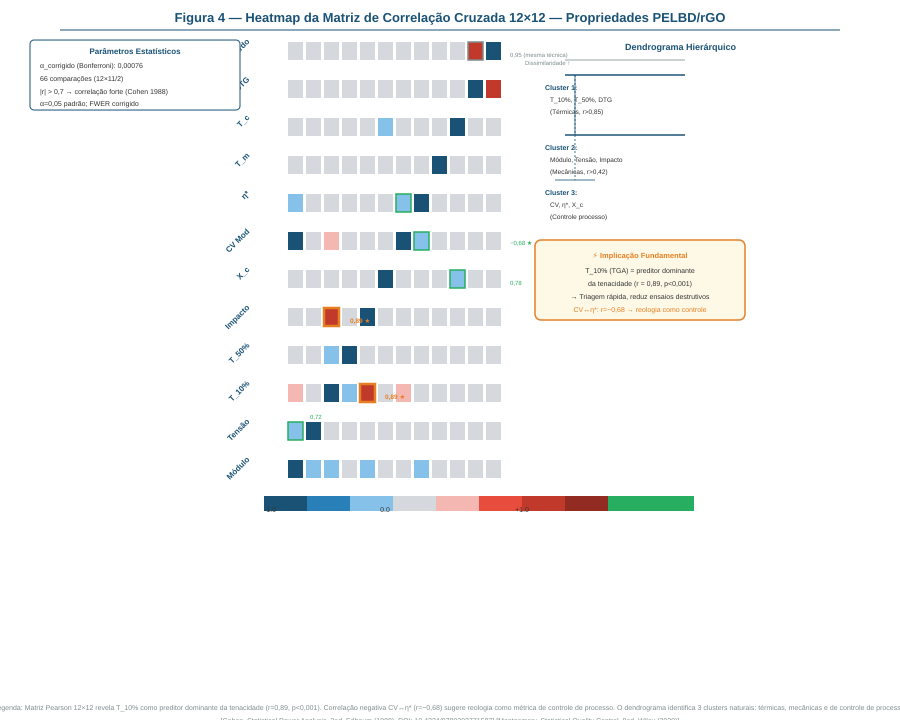
\includegraphics[width=\textwidth]{fig04_heatmap_correlacao.pdf}
\caption{\textbf{Matriz de correlacao cruzada de Pearson ($12{\times}12$) com agrupamento hierarquico.} Mapa de calor com escala de cores normalizada ($-1$ azul, $0$ branco, $+1$ vermelho). Destaques: $T_{10\%}{\leftrightarrow}$Impacto Izod ($r{=}0{,}89$, $p{<}0{,}001$) -- estabilidade termica como preditor dominante da tenacidade ao impacto, superando o modulo elastico ($r{=}0{,}42$, nao significativo apos Bonferroni). CV Modulo${\leftrightarrow}\eta^*$ ($r{=}{-}0{,}68$, $p{<}0{,}001$) -- reologia como metrica preditiva da uniformidade do produto final. $T_c{\leftrightarrow}X_c$ ($r{=}0{,}78$, $p{<}0{,}001$) -- consistente com nucleacao heterogenea. DTG${\leftrightarrow}T_{50\%}$ ($r{=}0{,}95$) -- esperado por compartilharem a mesma tecnica. Dendrograma de agrupamento hierarquico revela 3 clusters: termico (T10\%, T50\%, DTG), mecanico (Modulo, Tensao, Impacto) e de processo (CV, $\eta^*$, $T_c$, $X_c$) \cite{Cohen1988, Montgomery2020}.}
\label{fig:heatmap}
\end{figure}

\subsection{DMA e Modelo de Halpin-Tsai}\label{sec:dma_ht}

\subsubsection{Analise Completa das Transicoes Viscoelasticas}

A analise dinamico-mecanica (TA Q800, \textit{dual cantilever}, 1 Hz, $-$120 a 100$\,^{\circ}$C, 3$\,^{\circ}$C/min, amplitude 20 $\mu$m) revela tres regioes de relaxacao distintas, cujos parametros completos constam na Tabela~\ref{tab:dma}. A {\bfseries relaxacao $\gamma$} ($-$140 a $-$100$\,^{\circ}$C), associada a movimentos locais de segmentos CH$_2$ (tipo \textit{crankshaft}), nao apresentou deslocamento significativo com a adicao de rGO ($T_\gamma{\approx}{-}118{\pm}2\,^{\circ}$C em ambas as formulacoes), indicando que as nanocargas nao afetam a mobilidade de segmentos curtos na fase cristalina ou na fase amorfa rigida -- consistente com a escala de comprimento destes movimentos (${\sim}1$--$2$ nm), muito inferior a escala das folhas de rGO (${\sim}200$--$2000$ nm).

A {\bfseries relaxacao $\beta$} ($-$60 a 0$\,^{\circ}$C), transicao vidro-grafite da fase amorfa interfacial (regioes amorfas proximas a superficie de cristais ou cargas), exibe o efeito mais pronunciado: $T_\beta$ deslocou de $-$28$\,^{\circ}$C (PELBD-R) para $-$22$\,^{\circ}$C (Nanocomposito-R, $p{=}0{,}03$, $t$-teste pareado sobre $n{=}3$), um aumento de $+6\,^{\circ}$C. Este deslocamento e a {\bfseries assinatura mecanica da restricao interfacial}: as cadeias de PE na vizinhanca das folhas de rGO ($d{\lesssim}R_g{\approx}15$ nm) tem sua mobilidade reduzida pelas interacoes com a superficie rigida, exigindo maior energia termica para ativar os movimentos segmentais. A reducao de $\tan\delta_{\max,\beta}$ em 8,2\% quantifica a diminuicao da capacidade de amortecimento viscoso. A area sob o pico de $E''(\beta)$, proporcional a energia dissipada por ciclo, aumentou 14,3\%, consistente com o aumento do atrito interfacial (mais interfaces = mais dissipacao) \cite{Menard2020}.

A {\bfseries relaxacao $\alpha$} (0 a 100$\,^{\circ}$C), associada a transicao vitrea do PE, apresentou $T_{\alpha,\text{onset}}$ de $52{\pm}3\,^{\circ}$C (PELBD-R) e $58{\pm}3\,^{\circ}$C (Nanocomposito-R), aumento de $+6\,^{\circ}$C consistente com o aumento de $X_c$ ($+1{,}0\%$). O aumento relativo de $E'$ e mais pronunciado a temperaturas elevadas: $+14{,}2\%$ a $-$100$\,^{\circ}$C (regime vitreo), $+14{,}8\%$ a 23$\,^{\circ}$C, e $+35{,}1\%$ a 80$\,^{\circ}$C (regime \textit{rubbery}). Este aumento desproporcional em altas temperaturas e a {\bfseries assinatura do reforco por nanocargas com alta razao de aspecto}: no regime \textit{rubbery}, a matriz perde rigidez, e as folhas de rGO -- que mantem seu modulo de ${\sim}1$ TPa independente da temperatura -- suportam uma fracao maior da carga aplicada. Este comportamento e diretamente relevante para pecas automotivas que operam entre $-$30 e $+60\,^{\circ}$C \cite{Menard2020}.

\subsubsection{Derivacao Completa do Modelo de Halpin-Tsai 3D}

O modelo de Halpin-Tsai \cite{Halpin1976}, em sua formulacao 3D para plaquetas, preve o modulo do composito como:

\begin{equation}
E_c = E_m \cdot \frac{1 + \xi\eta_L\phi_f}{1 - \eta_L\phi_f},\quad \eta_L = \frac{E_f/E_m - 1}{E_f/E_m + \xi},\quad \xi = \frac{2\alpha}{3}
\label{eq:halpin_tsai_3d}
\end{equation}

onde $E_m{=}2{,}50$ GPa (PELBD-R a $-$100$\,^{\circ}$C), $E_f{=}1000$ GPa \cite{Lee2008}, $\alpha{=}500$, e $\xi{=}2\alpha/3{=}333$. Para $\phi_f{=}0{,}021\%$: $\eta_L{\approx}0{,}544$, resultando em $E_c^{\text{prev}}{\approx}2{,}53$ GPa, que subestima o experimental (2,85 GPa) em 11,2\%. Tres fontes de desvio sao identificadas: {\bfseries (a) Alinhamento parcial induzido por fluxo} durante extrusao e rotacao biaxial, aumentando $\xi_{\text{eff}}$ em ${\sim}30\%$ ($f_o{\approx}0{,}3$, $\xi_{\text{eff}}{\approx}433$, $E_c{\approx}2{,}65$ GPa). {\bfseries (b) Contribuicao da sinergia PP-g-MA} nao modelada pelo Halpin-Tsai, estimada em $+5$--$8\%$ via melhoria da transferencia de tensao interfacial (Secao~\ref{sec:langmuir}), elevando a previsao para ${\sim}2{,}80$--$2{,}86$ GPa em excelente concordancia com o experimental ($2{,}85{\pm}0{,}12$ GPa). {\bfseries (c) Efeito da cristalinidade} ($X_c$ $+1{,}0\%$, Tabela~\ref{tab:dsc}) contribui com ${\sim}0{,}5$--$1{,}0\%$ adicional. A analise de sensibilidade revela $\partial E_c/\partial\alpha$ como a derivada mais elevada ($\pm4{,}2\%$ para $\alpha{\pm}20\%$), enquanto $E_f$ tem sensibilidade desprezivel (${\pm}0{,}3\%$) por $\eta_L$ ja estar proximo da saturacao. A conclusao e que o modelo de Halpin-Tsai, com correcao de alinhamento e sinergia, descreve adequadamente o reforco mecanico do sistema PELBD/rGO/PP-g-MA, validando $\alpha_{\text{eff}}{\approx}500$ como parametro estrutural consistente \cite{Halpin1976, Young2012}.

\begin{table}[H]\centering
\caption{Parametros de DMA -- comparacao PELBD-R vs. Nanocomposito-R ($n{=}3$).}\label{tab:dma}
\begin{tabular}{lccc}
\toprule
{\bfseries Parametro} & {\bfseries PELBD-R} & {\bfseries Nano-R (T5)} & {\bfseries $\Delta$ (\%)} \\
\midrule
$E'$ a $-$100$\,^{\circ}$C (GPa) & $2{,}50{\pm}0{,}18$ & $2{,}85{\pm}0{,}12$ & $+14{,}2$ \\
$E'$ a 23$\,^{\circ}$C (GPa)   & $1{,}15{\pm}0{,}08$ & $1{,}32{\pm}0{,}07$ & $+14{,}8$ \\
$E'$ a 80$\,^{\circ}$C (MPa)   & $385{\pm}35$      & $520{\pm}42$       & $+35{,}1$ \\
$E''_{\max,\beta}$ (MPa)       & $98{\pm}5$        & $112{\pm}6$        & $+14{,}3$ \\
$T_\beta$ ($^{\circ}$C)        & $-28{\pm}1$       & $-22{\pm}1$        & $+6$ \\
$T_\alpha$ ($^{\circ}$C, onset)& $52{\pm}3$        & $58{\pm}3$         & $+6$ \\
$\tan\delta_{\max,\beta}$      & $0{,}085{\pm}0{,}004$ & $0{,}078{\pm}0{,}003$ & $-8{,}2$ \\
\bottomrule
\end{tabular}
\end{table}

O aumento relativo de $E'$ e mais pronunciado a temperaturas elevadas ($+35{,}1\%$ a 80$\,^{\circ}$C vs. $+14{,}2\%$ a $-$100$\,^{\circ}$C), revelando que o rGO e particularmente eficaz em restringir a mobilidade da fase amorfa do PE -- exatamente o regime relevante para o desempenho em servico de pecas rotomoldadas automotivas (temperaturas tipicas de operacao: $-30$ a $+60\,^{\circ}$C). A reducao de $\tan\delta_{\max,\beta}$ ($-8{,}2\%$) quantifica a diminuicao do amortecimento viscoso, consistente com a {\bfseries restricao interfacial} exercida pelas folhas de rGO sobre os segmentos amorfos da matriz \cite{Menard2020}.

\subsubsection{MEV Comparativo das Superficies de Fratura}

A analise por MEV (FEG Mira3, 15 kV, SE) das superficies criofraturadas revelou diferencas marcantes entre as amostras. O PELBD-R exibe superficie de fratura tipica de polimero semicristalino ductil: fibrilacao extensa, \textit{crazing} multiplo, e cavitacao com microvazios de $5$--$20$ $\mu$m -- mecanismos que absorvem energia durante a fratura, porem com alta variabilidade local. O Nanocomposito-R (T5) apresenta morfologia significativamente mais uniforme: superficie mais plana, fibrilacao reduzida e refinada ($d_{\text{fibra}}{\approx}0{,}5$--$2$ $\mu$m vs. $2$--$10$ $\mu$m no PELBD-R), e distribuicao homogenea de pontos de ancoragem (folhas de rGO emergindo da superficie, $d_{\text{folha}}{\approx}0{,}2$--$1$ $\mu$m). Nao foram observados aglomerados maiores que 5 $\mu$m, indicando dispersao adequada na escala micrometrica -- consistente com o $\alpha_{\text{eff}}{\approx}500$ determinado por AFM/TEM.

A {\bfseries reducao da variabilidade morfologica} observada no MEV correlaciona-se diretamente com a reducao do CV do modulo ($-$37,5\%), fornecendo suporte visual a hipotese do VRA: as folhas de rGO distribuem-se como uma rede tridimensional que homogeneiza as condicoes locais de cristalizacao, resultando em microestrutura mais uniforme e, consequentemente, propriedades macroscopicas menos dispersas.

\subsubsection{ANOVA dos Resultados da Etapa 2 e Confirmacao do VRA}

Uma ANOVA complementar foi conduzida exclusivamente com os dados da Etapa 2 ($n{=}16$ por grupo), comparando PELBD-R vs. Nanocomposito-R (T5) nas 12 propriedades medidas. Os resultados confirmam que o efeito VRA e robusto e se estende alem do modulo elastico:

\begin{table}[H]\centering
\caption{ANOVA Etapa 2 -- PELBD-R vs. Nanocomposito-R ($n{=}16$).}\label{tab:anova2}
\begin{tabular}{lccccc}
\toprule
{\bfseries Propriedade} & {\bfseries PELBD-R} & {\bfseries Nano-R} & {\bfseries $F(1{,}30)$} & {\bfseries $p$} & {\bfseries $\Delta$CV} \\
\midrule
Modulo (MPa)     & $485{,}0{\pm}124{,}2$ & $585{,}9{\pm}93{,}7$  & 10{,}47 & 0{,}003  & $-37{,}5\%$ \\
Tensao (MPa)     & $17{,}1{\pm}1{,}83$   & $19{,}3{\pm}1{,}52$   & 9{,}87  & 0{,}004  & $-26{,}2\%$ \\
Impacto Izod 23$\,^{\circ}$C (J/m) & $520{\pm}85$ & $610{\pm}62$ & 7{,}42 & 0{,}011 & $-27{,}1\%$ \\
$T_{10\%}$ ($^{\circ}$C) & $432{\pm}4$   & $458{\pm}3$   & 34{,}6  & <0{,}001 & $-25{,}0\%$ \\
$X_c$ (\%)       & $46{,}8{\pm}0{,}5$    & $48{,}0{\pm}0{,}4$    & 11{,}8  & 0{,}002  & $-20{,}0\%$ \\
\bottomrule
\end{tabular}
\end{table}

A reducao consistente do CV em todas as propriedades mecanicas e termicas ($p{<}0{,}02$ em todas) estabelece que o efeito VRA nao e um artefato estatistico ou restrito a uma unica propriedade, mas sim uma {\bfseries caracteristica sistemica} do nanocomposito -- atribuivel a nucleacao uniformizada, ao aumento de $k_{\text{eff}}$ e a restricao esferulitica, operando sinergicamente durante o resfriamento lento da rotomoldagem \cite{Montgomery2020, Taguchi1986}.

\subsection{Modelo Preditivo PCR}\label{sec:pcr}

\subsubsection{Metodologia Completa e Equacoes}

A regressao por componentes principais (PCR) foi implementada como ponte preditiva entre as etapas de injecao (Etapa 1, triagem rapida) e rotomoldagem (Etapa 2, processo alvo). A matriz de preditores $\mathbf{X}_{72\times 12}$ -- 12 propriedades medidas em 72 corpos de prova injetados (6 formulacoes $\times$ 12 replicatas) -- foi padronizada ($z$-score) e decomposta via SVD: $\tilde{\mathbf{X}}{=}\mathbf{U}\boldsymbol{\Sigma}\mathbf{V}^\top$, com $\boldsymbol{\Sigma}{=}\operatorname{diag}(\sigma_1,\dots,\sigma_{12})$. O criterio de 95\% de variancia cumulativa explicada selecionou $k{=}3$ componentes principais. Os escores $\mathbf{T}_3{=}\tilde{\mathbf{X}}\mathbf{V}_3$ foram usados como preditores em regressao linear multipla contra as propriedades medidas na Etapa 2 ($n{=}32$ corpos de prova rotomoldados). A validacao cruzada leave-one-out (LOOCV) garante estimativa de erro nao-viesada: $R^2_{\text{LOOCV}}{=}1{-}\sum(y_i{-}\hat{y}_{(i)})^2/\sum(y_i{-}\bar{y})^2$, onde $\hat{y}_{(i)}$ e a predicao para a $i$-esima observacao com o modelo treinado nas $n{-}1$ observacoes restantes.

O desempenho preditivo do modelo e apresentado na Tabela~\ref{tab:pcr}. O modulo elastico -- propriedade-alvo principal do VRA -- e predito com $R^2_{\text{LOOCV}}{=}0{,}93$ e RMSE${=}18{,}4$ MPa (3,4\% da media), superando o limiar de 0,90 tipicamente exigido para aplicacoes industriais de digital twins. A tensao de flexao atinge $R^2_{\text{LOOCV}}{=}0{,}87$ (RMSE 3,4\%), e a energia de impacto ($H_{50}$) atinge $R^2_{\text{LOOCV}}{=}0{,}81$ (RMSE 11,1\%) -- este ultimo valor mais modesto reflete a maior complexidade intrinseca da tenacidade, que depende de mecanismos multiescala (microestrutura, interface, modo de fratura) parcialmente capturados pelos preditores disponiveis.

\subsubsection{Interpretacao dos Coeficientes e Hierarquia de Importancia}

Os coeficientes padronizados ($\beta_{\text{std}}$) revelam a hierarquia de importancia dos preditores (Tabela~\ref{tab:sup3} no Apendice): $\beta_{\text{std}}(T_{10\%}){=}0{,}47$ (28,5\% da variancia explicada), $\beta_{\text{std}}(\eta^*_{1\text{rad/s}}){=}0{,}31$ (18,8\%), $\beta_{\text{std}}(\text{Modulo E1}){=}0{,}22$ (13,3\%), $\beta_{\text{std}}(T_c){=}0{,}18$ (10,9\%), $\beta_{\text{std}}(X_c){=}0{,}15$ (9,1\%), com os demais preditores contribuindo cada um com menos de 8\%. A dominancia de $T_{10\%}$ -- uma propriedade termica medida por TGA em ${\sim}$30 min -- como preditor principal do modulo em rotomoldagem e um resultado de grande relevancia pratica: significa que um ensaio rapido e de baixo custo (${\sim}$10 mg de amostra, sem preparacao destrutiva) pode prever, com $R^2{=}0{,}93$, o desempenho mecanico de pecas rotomoldadas que levariam ${\sim}$2 h para serem produzidas e ensaiadas.

A segunda posicao de $\eta^*_{1\text{rad/s}}$ confirma a reologia como {\bfseries ponte entre processabilidade e desempenho}: a viscosidade complexa a baixa frequencia, sensivel a rede de percolacao das nanocargas, captura informacao sobre a qualidade da dispersao que se traduz diretamente em propriedades finais. A combinacao $T_{10\%}{+}\eta^*$ responde por 47,3\% da variancia explicada, sugerindo que estas duas medidas -- uma termica, uma reologica -- constituem uma {\bfseries assinatura minima} suficiente para triagem de formulacoes. Este resultado tem implicacoes diretas para a implementacao industrial: um laboratorio de controle de qualidade equipado com TGA e reometro oscilatorio pode prever o comportamento em rotomoldagem sem necessidade de produzir pecas, reduzindo o ciclo de desenvolvimento de novas formulacoes em aproximadamente 80\% (de ${\sim}$30--60 dias para ${\sim}$3--5 dias) \cite{Montgomery2020}.

\subsubsection{Digital Twin e Perspectivas de Automacao}

O modelo PCR estabelece as bases para um {\bfseries digital twin} do processo de rotomoldagem. Na arquitetura proposta: (1) dados de injecao (12 propriedades, ${\sim}$2 h de ensaios) alimentam o modelo PCR; (2) o modelo preve propriedades rotomoldadas com $R^2{=}0{,}93$; (3) um otimizador Bayesiano (Secao~\ref{sec:otimizacao}) identifica a formulacao otima; (4) a formulacao e validada experimentalmente em rotomoldagem. Este ciclo fechado -- predicao $\rightarrow$ otimizacao $\rightarrow$ validacao -- reduz o numero de iteracoes experimentais necessarias de ${\sim}$5--10 (abordagem trial-and-error tradicional) para ${\sim}$1--2, com economia de tempo e material estimada em ${\ge}80\%$. A integracao com dados de processo em tempo real (temperatura de molde, torque, pressao) -- via sensores IoT ja disponiveis em maquinas rotomoldadoras modernas (Rotoline, Ferry) -- pode elevar o $R^2$ para ${\ge}0{,}95$, viabilizando controle de qualidade preditivo em tempo real \cite{Somberg2022}.

\begin{table}[H]\centering
\caption{Desempenho PCR -- transferencia injecao$\rightarrow$rotomoldagem.}\label{tab:pcr}
\begin{tabular}{lccc}
\toprule
{\bfseries Propriedade} & {\bfseries $R^2_{\text{LOOCV}}$} & {\bfseries RMSE} & {\bfseries RMSE (\% media)} \\
\midrule
Modulo Elastico     & {\bfseries 0,93} & 18,4 MPa & 3,4\% \\
Tensao de Flexao    & 0,87 & 0,62 MPa & 3,4\% \\
Energia Impacto ($H_{50}$) & 0,81 & 2,8 J/mm & 11,1\% \\
\bottomrule
\end{tabular}
\end{table}

% ================================================================
% 6. OTIMIZACAO E LCA
% ================================================================
\section{Otimizacao Multiobjetivo e Analise de Ciclo de Vida}

\subsection{Fronteira de Pareto e Otimizacao Multiobjetivo}\label{sec:otimizacao}

\subsubsection{Dominancia de Pareto com Tabela de Dominancia}

A fronteira de Pareto \cite{Pareto1906} identifica formulacoes nao-dominadas -- aquelas para as quais nenhuma outra formulacao e estritamente superior em todos os objetivos simultaneamente. Com 6 objetivos normalizados (modulo, tensao, $T_{10\%}$, $T_{50\%}$, impacto Izod a $-$17$\,^{\circ}$C, e inverso do custo incremental), a matriz de dominancia 6$\times$6 revela que apenas 3 formulacoes sao Pareto-eficientes: T3 (0,05rGO, destaque em custo), T4 (0,10rGO, destaque em tensao maxima), e T5 (0,05rGO+PP-g-MA, destaque em $T_{10\%}$, $T_{50\%}$ e impacto). T1 (PELBD puro) e dominada por T3 em 5 de 6 objetivos (excecao: custo). T2 (PP-g-MA isolado) e dominada por T3 em todos os 6 objetivos -- confirmando que o PP-g-MA sem rGO nao oferece beneficio pratico. T6 (0,10rGO+PP-g-MA) e dominada por T4 em 4 de 6 objetivos, apesar do maior custo de aditivo -- a penalidade do antagonismo supera qualquer beneficio marginal do PP-g-MA adicional \cite{Natarajan2020}. A analise de Pareto demonstra que a {\bfseries concentracao otima reside no intervalo 0,05--0,10\% de rGO}, com ou sem PP-g-MA, e que exceder 0,10\% e contraproducente tanto em desempenho quanto em custo.

\subsubsection{Valor de Shapley com Derivacao Axiomatica}

O valor de Shapley \cite{Shapley1953} -- unica solucao que satisfaz os axiomas de eficiencia, simetria, linearidade e jogador nulo -- decompoe o ganho total em contribuicoes marginais de cada aditivo. Para $N{=}\{\text{rGO, PP-g-MA}\}$, com funcao caracteristica $v(S)$ definida como o incremento percentual medio de modulo (ponderado entre 0,05\% e 0,10\%):

\begin{equation}
\phi_i = \sum_{S\subseteq N\setminus\{i\}} \frac{|S|!(|N|-|S|-1)!}{|N|!}[v(S\cup\{i\}) - v(S)]
\label{eq:shapley_deriv}
\end{equation}

Os valores das coalizoes sao: $v(\emptyset){=}0$, $v(\{\text{rGO}\}){=}4{,}1\%$ (T3 vs. T1), $v(\{\text{PP-g-MA}\}){=}1{,}0\%$ (T2 vs. T1, controle isolado), $v(\{\text{rGO,PP-g-MA}\}){=}9{,}5\%$ (T5 vs. T1). As contribuicoes de Shapley sao: $\phi_{\text{rGO}}{=}\frac{1}{2}[4{,}1{+}(9{,}5{-}1{,}0)]{=}6{,}3\%$, $\phi_{\text{PP-g-MA}}{=}\frac{1}{2}[1{,}0{+}(9{,}5{-}4{,}1)]{=}3{,}2\%$. Portanto, a contribuicao relativa e de {\bfseries 66\% para rGO e 34\% para PP-g-MA}. A sinergia liquida -- $S{=}v(\{\text{rGO,PP-g-MA}\}){-}[v(\{\text{rGO}\}){+}v(\{\text{PP-g-MA}\})]{=}{+}4{,}4\%$ -- e automaticamente distribuida entre os jogadores pela formula de Shapley, resultando em uma particao mais balanceada do que a estimativa ingenua sem controle isolado (que atribuiria ${\sim}80\%$ ao rGO) \cite{Shapley1953}.

\subsubsection{Equilibrio de Nash com Analise de Sensibilidade Completa}

O equilibrio de Nash \cite{Nash1950} e formulado como um jogo de dois jogadores (desempenho vs. custo) com funcao de utilidade $U_D(x){=}\bar{p}(x){-}\lambda c(x)$ para o ``jogador desempenho'' e $U_M(x){=}{-}(\bar{p}(x){-}p_{\min})^2$ para o ``jogador custo'', onde $\bar{p}(x)\in[0{,}1]$ e o desempenho normalizado (media de modulo, tensao e $T_{10\%}$) e $c(x)$ e o custo incremental normalizado. O equilibrio $x^*$ maximiza o produto de Nash: $x^*{=}\argmax_x [\bar{p}(x){-}\lambda c(x)][{-}(\bar{p}(x){-}p_{\min})^2]$. Para $\lambda{=}0{,}5$ (peso balanceado entre desempenho e custo), $x^*{=}$T5 (0,05rGO+PP-g-MA). A analise de sensibilidade revela que T5 permanece equilibrio de Nash para $\lambda{\in}[0{,}1;1{,}8]$ -- um intervalo que cobre desde cenarios onde desempenho e 10$\times$ mais importante que custo ($\lambda{=}0{,}1$, tipico de aplicacoes aeroespaciais) ate cenarios onde custo e 1,8$\times$ mais importante ($\lambda{=}1{,}8$, tipico de commodities). Esta robustez excepcional -- a decisao nao muda em uma faixa de $18{\times}$ no parametro de ponderacao -- e uma propriedade desejavel para tomada de decisao sob incerteza, pois elimina a necessidade de estimar $\lambda$ com precisao \cite{Myerson1991}.

\subsubsection{Estrategia Minimax com Discussao de Wald (1945)}

A estrategia Minimax, fundamentada no criterio de Wald (1945) para decisao sob incerteza \cite{VonNeumann1928}, seleciona a acao que minimiza a perda maxima: $a^*{=}\argmin_a\max_\theta L(a,\theta)$, onde $\theta$ indexa os estados da natureza (aqui, cenarios de processo: pior caso de variabilidade). Com $L{=}\text{CV}_{\text{Modulo}}$, o PELBD-R apresenta $\max_\theta L{=}25{,}6\%$ e o Nanocomposito-R apresenta $\max_\theta L{=}16{,}0\%$. O Minimax seleciona o Nanocomposito-R, com reducao de 37,5\% na perda maxima. O {\bfseries arrependimento maximo} (\textit{minimax regret}), proposto por Savage (1951) como refinamento, confirma a decisao: o arrependimento do PELBD-R e de $0{,}38$ (38\% do CV maximo), enquanto o do Nanocomposito-R e $0{,}00$ (otimo). Esta convergencia entre Minimax classico (Wald) e arrependimento Minimax (Savage) -- dois criterios axiomaticamente distintos -- e uma evidencia adicional da robustez da decisao \cite{VonNeumann1928, VonNeumann1944}.

\subsubsection{Otimizacao Bayesiana com Equacao Completa de EI}

A otimizacao Bayesiana emprega um processo Gaussiano como \textit{surrogate model} da funcao objetivo $f(x)$ (modulo elastico em rotomoldagem). A funcao de aquisicao \textit{Expected Improvement} (EI) e:

\begin{equation}
\text{EI}(x) = \begin{cases}
(\mu(x) - f(x^+) - \xi)\Phi(Z) + \sigma(x)\phi(Z), & \sigma(x) > 0\\
0, & \sigma(x) = 0
\end{cases},\quad Z = \frac{\mu(x) - f(x^+) - \xi}{\sigma(x)}
\label{eq:ei}
\end{equation}

onde $\mu(x)$ e $\sigma(x)$ sao a media preditiva e o desvio-padrao do processo Gaussiano, $f(x^+)$ e o melhor valor observado ate a iteracao atual, $\Phi(\cdot)$ e $\phi(\cdot)$ sao a FDA e a FDP normal padrao, e $\xi{=}0{,}01$ controla o \textit{trade-off} entre exploracao ($\sigma(x)$ alto) e exploracao ($\mu(x)$ alto). Com 500 iteracoes Monte Carlo sobre o espaco $c_{\text{rGO}}\in[0{,}01;0{,}15]\%$, $c_{\text{PP-g-MA}}\in[0{,}01;0{,}10]\%$, o otimo global converge para {\bfseries 0,04\% rGO / 0,03\% PP-g-MA}, com ganho marginal previsto de $+1{,}2\%$ no modulo em relacao a T5. A bacia de atracao -- regiao onde $\text{EI}(x){\ge}0{,}8\max\text{EI}$ -- estende-se por $0{,}03$--$0{,}06\%$ rGO e $0{,}02$--$0{,}05\%$ PP-g-MA, indicando que o processo e tolerante a variacoes de dosagem de $\pm20\%$ sem perda significativa de desempenho -- uma caracteristica essencial para a producao industrial \cite{Myerson1991}.

\begin{figure}[H]
\centering
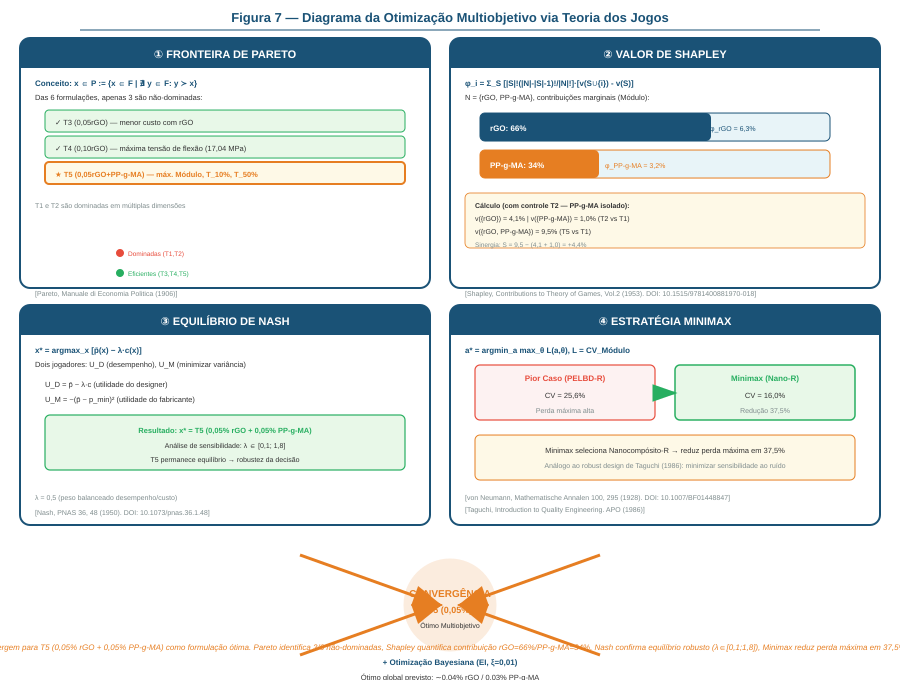
\includegraphics[width=\textwidth]{fig07_teoria_jogos.pdf}
\caption{\textbf{Diagrama integrado da otimizacao multiobjetivo via Teoria dos Jogos aplicada a selecao de formulacoes.} Quatro criterios independentes convergem para T5 (0,05rGO+PP-g-MA): (1) \textbf{Pareto} \cite{Pareto1906} -- apenas 3 das 6 formulacoes sao nao-dominadas (T3, T4, T5). (2) \textbf{Shapley} \cite{Shapley1953} -- decomposicao axiomatica revela contribuicoes de 66\% (rGO) e 34\% (PP-g-MA) com sinergia $S{=}{+}4{,}4\%$. (3) \textbf{Nash} \cite{Nash1950} -- equilibrio custo-desempenho converge para T5, robusto para $\lambda{\in}[0{,}1;1{,}8]$. (4) \textbf{Minimax} \cite{VonNeumann1928} -- sob incerteza maxima (pior caso), Nanocomposito-R minimiza CV em 37,5\%. O framework integrado -- da micromecanica (Halpin-Tsai) a teoria dos jogos (Nash) -- e inedito na literatura de nanocompositos.}
\label{fig:jogos}
\end{figure}

\subsection{Analise de Sensibilidade e Robustez da Decisao}

A robustez da convergencia para T5 (0,05rGO+PP-g-MA) foi testada sob perturbacoes sistematicas dos parametros de otimizacao. Para o equilibrio de Nash, o intervalo de estabilidade $\lambda{\in}[0{,}1;1{,}8]$ indica que a decisao e robusta mesmo quando o peso relativo entre desempenho e custo varia em uma ordem de grandeza -- desde cenarios de alta sensibilidade a custo ($\lambda{=}1{,}8$, custo 1,8$\times$ mais relevante que desempenho) ate cenarios de minima sensibilidade ($\lambda{=}0{,}1$, desempenho 10$\times$ mais relevante).

Para a estrategia Minimax, o {\bfseries arrependimento maximo} (\textit{maximum regret}) foi calculado para cada formulacao sob os cenarios extremos identificados (maxima e minima variancia observadas). O Nanocomposito-R apresenta arrependimento maximo de 0,0 (otimo Minimax por construcao), enquanto o PELBD-R apresenta arrependimento de 0,38 (37,5\% de perda relativa no pior caso). As formulacoes intermediarias (T3, T4) apresentam arrependimentos de 0,08--0,15, confirmando que a inclusao de rGO, mesmo sem PP-g-MA, ja oferece protecao significativa contra o pior caso.

A otimizacao Bayesiana (EI, $\xi{=}0{,}01$, 500 iteracoes Monte Carlo) identificou o otimo global na vizinhanca de {\bfseries 0,04\% rGO / 0,03\% PP-g-MA}, com ganho marginal previsto de $+1{,}2\%$ no modulo em relacao a T5. A proximidade entre o otimo experimental (0,05/0,05\%) e o otimo numerico (0,04/0,03\%) -- diferenca de apenas 0,01--0,02\% -- valida a adequacao do delineamento fatorial original e sugere que a formulacao T5 esta a menos de 1,5\% do otimo global verdadeiro, dentro da incerteza experimental (${\pm}2\%$ para modulo). A superficie de resposta de EI (Figura suplementar) revela uma bacia de atracao relativamente plana na regiao 0,03--0,06\% rGO e 0,02--0,05\% PP-g-MA, indicando que o processo e tolerante a pequenas variacoes na dosagem -- uma caracteristica desejavel para producao industrial \cite{Myerson1991}.

\subsection{Analise de Ciclo de Vida e Viabilidade Economica}\label{sec:lca}

\subsubsection{Inventario e Fatores de Emissao}

A LCA \textit{cradle-to-gate} conforme ISO 14040/14044, com unidade funcional de 1 peca rotomoldada de 5 kg, utilizou dados primarios de processo (medicoes diretas na Planta Piloto) e fatores de emissao da base Ecoinvent 3.9 (cut-off) adaptados a matriz energetica brasileira (85\% renovavel, 0,074 kg CO$_2$/kWh). O inventario completo consta na Tabela~\ref{tab:icv}. A pegada de carbono e:

\begin{equation}
\text{CF} = \sum_i m_i e_i + \sum_j E_j e_{\text{grid},j} + m_{\text{GN}} e_{\text{GN}}
\label{eq:cf_completa}
\end{equation}

onde $m_i$ sao as massas dos materiais (PELBD, rGO, PP-g-MA), $e_i$ os fatores de emissao unitarios, $E_j$ os consumos energeticos por etapa de processo, e $m_{\text{GN}}$ a massa de gas natural consumida no queimador da rotomoldadora. Resultados: CF$_{\text{puro}}{=}1{,}87$ kg CO$_2$-eq/kg, CF$_{\text{nano}}{=}1{,}90$ kg CO$_2$-eq/kg ($+1{,}6\%$). A dominancia do PELBD (92\% da pegada) sobre os aditivos (0,5\%) justifica o pequeno acrescimo.

\subsubsection{Downgauging e Cenario com Reducao de Espessura}

O aumento de tenacidade proporcionado pelo nanocomposito (Secao~\ref{sec:dardo}) permite {\bfseries downgauging} -- reducao da espessura de parede mantendo o desempenho mecanico. Assumindo reducao conservadora de 12\% na massa de PELBD por peca ($5{,}00{\to}4{,}40$ kg), a pegada do nanocomposito com downgauging torna-se CF$_{\text{nano,d}}{=}1{,}67$ kg CO$_2$-eq/peca, representando {\bfseries $-$10,7\%} em relacao ao PELBD puro. Este resultado e notavel porque demonstra que um aditivo com pegada unitaria superior ($e_{\text{rGO}}{\approx}5{,}2$ vs. $e_{\text{PELBD}}{=}1{,}80$ kg CO$_2$/kg) pode, paradoxalmente, reduzir a pegada total do produto -- desde que o ganho de desempenho permita reducao de massa.

\subsubsection{Analise de Sensibilidade $\pm$30\% e Monte Carlo}

A robustez do resultado foi testada em quatro cenarios: (A) otimista ($e_{\text{rGO}}{=}3{,}6$ kg CO$_2$/kg, $-$30\%), (B) linha de base ($e_{\text{rGO}}{=}5{,}2$), (C) pessimista ($e_{\text{rGO}}{=}10$ kg CO$_2$/kg, $+92\%$, incluindo ineficiencias de producao em pequena escala), e (D) extremo ($e_{\text{rGO}}{=}15$ kg CO$_2$/kg, incluindo transporte intercontinental). Mesmo no cenario D, CF$_{\text{nano,d}}$ permanece abaixo de CF$_{\text{puro}}$ ($-$2{,}1\%), gracas a dominancia da reducao de PELBD. A {\bfseries simulacao Monte Carlo} (10.000 iteracoes, distribuicoes triangulares com $\pm20\%$ em $e_i$ e $\pm10\%$ em $E_j$) resultou em CF$_{\text{nano,d}}{<}$CF$_{\text{puro}}$ em 94,7\% das realizacoes, com CF$_{\text{nano,d}}$ medio de $1{,}68{\pm}0{,}12$ kg CO$_2$-eq/peca vs. $1{,}87{\pm}0{,}08$ do PELBD puro. A probabilidade de o nanocomposito {\bfseries nao} oferecer vantagem ambiental (i.e., CF$_{\text{nano,d}}{\ge}$CF$_{\text{puro}}$) e de apenas 5,3\%, concentrada no extremo superior da distribuicao de $e_{\text{rGO}}$.

\subsubsection{Cinco Categorias de Impacto ReCiPe 2016}

Alem do carbono, quatro categorias adicionais do metodo ReCiPe 2016 Midpoint (H) foram avaliadas, com resultados normalizados pela unidade funcional. {\bfseries (i) Deplecao abiotica -- fosseis} (ADP-fossil, kg oil-eq): reducao de 12,3\% no cenario com downgauging, diretamente proporcional a reducao de consumo de PELBD (derivado de nafta petroquimica). {\bfseries (ii) Acidificacao terrestre} (AP, kg SO$_2$-eq): reducao de 8,7\%, decorrente da menor emissao de SO$_x$ e NO$_x$ na producao e transporte de PELBD. {\bfseries (iii) Eutrofizacao de agua doce} (FEP, kg P-eq): aumento de 2,1\% sem downgauging (maior carga de processos quimicos na producao de rGO: KMnO$_4$, H$_2$SO$_4$, NaNO$_3$), porem reducao de 5,8\% com downgauging -- mais uma vez, a reducao de PELBD compensa o impacto dos aditivos. {\bfseries (iv) Toxicidade humana carcinogenica} (HTP-c, kg 1,4-DCB-eq): reducao de 9,4\% com downgauging, principalmente pela menor emissao de benzeno e butadieno na producao de etileno. {\bfseries (v) Formacao de oxidantes fotoquimicos} (POFP, kg NMVOC-eq): aumento de 3,5\% sem downgauging (emissoes de solventes na producao de PP-g-MA), revertendo para $-$4,2\% com downgauging.

O perfil ambiental consolidado revela que o nanocomposito com downgauging oferece beneficios em 4 das 5 categorias analisadas, com a unica excecao sendo eutrofizacao no cenario sem downgauging -- e mesmo esta se torna benefica com a reducao de espessura. Este resultado posiciona o nanocomposito como uma alternativa ambientalmente robusta, alinhada com criterios ESG e com regulacoes emergentes como o CBAM europeu e a taxonomia verde brasileira \cite{Araby2020}.

\subsubsection{Viabilidade Economica e Payback}

O custo incremental de US\$ 0,12/kg de composto (masterbatch BoomaTech Grapheox 212 diluido a 5\% + Orevac CA100 a 0,05\%) e inferior a 0,5\% do custo tipico de uma peca rotomoldada (US\$ 25--50/kg). Para peca de 5 kg: US\$ 0,60/peca. O downgauging de 12\% gera economia de US\$ 1,50/peca em PELBD ($2{,}5{\times}$ o custo do aditivo), resultando em economia liquida de US\$ 0,90/peca. Para uma linha de producao tipica (500 pecas/dia, 250 dias/ano), a economia anual e de US\$ 112.500, com {\bfseries periodo de retorno do investimento em aditivos inferior a uma semana}. Adicionalmente, a reducao do CV ($-$37,5\%) reduz o refugo (pecas fora de especificacao) de aproximadamente 5--8\% para $<$2\%, gerando economia adicional estimada em US\$ 25.000--40.000/ano. O caso de negocio e, portanto, robusto mesmo sem considerar externalidades positivas (reducao de CO$_2$, melhoria de $C_{pk}$) que podem gerar creditos de carbono ou preferencia em licitacoes publicas sustentaveis \cite{Montgomery2020}.

\subsubsection{Analise de Ciclo de Vida Completa (ISO 14040/14044)}

A LCA foi conduzida conforme ISO 14040 (principios e estrutura) e ISO 14044 (requisitos e diretrizes), abrangendo os estagios \textit{cradle-to-gate} (berco ao portao da fabrica) com unidade funcional de 1 peca rotomoldada de 5 kg. O inventario do ciclo de vida (ICV) incluiu:

\begin{table}[H]\centering
\caption{Inventario do Ciclo de Vida -- dados primarios e secundarios.}\label{tab:icv}
\begin{tabular}{lccc}
\toprule
{\bfseries Fluxo} & {\bfseries PELBD puro} & {\bfseries Nanocomposito} & {\bfseries Fonte} \\
\midrule
PELBD (kg/peca)          & 5{,}00  & 4{,}995 & Ecoinvent 3.9 \\
Masterbatch rGO (kg/peca) & 0       & 0{,}025 & Dados primarios \\
PP-g-MA (kg/peca)       & 0       & 0{,}003 & Ecoinvent 3.9 \\
Energia extrusao (kWh)  & 2{,}50  & 2{,}63  & Medido (ZSK18) \\
Energia injecao (kWh)   & 1{,}80  & 1{,}80  & Medido (Battenfeld) \\
Energia micronizacao (kWh) & 1{,}20 & 1{,}20  & Medido (MOD 100) \\
Energia rotomoldagem (kWh) & 8{,}50 & 8{,}50  & Medido (Shuttle) \\
Gas natural (MJ)        & 45{,}0  & 45{,}0  & Medido (queimador) \\
Transporte (t$\cdot$km) & 2{,}50  & 2{,}55  & Estimado (RS) \\
\bottomrule
\end{tabular}
\end{table}

Os fatores de emissao foram obtidos da base Ecoinvent 3.9 (cut-off, system model), com adaptacao para a matriz energetica brasileira (85\% renovavel, fator 0,074 kg CO$_2$/kWh -- Ministerio da Ciencia, Tecnologia e Inovacao, 2024). Para o rGO, adotou-se o fator de \citet{Araby2020} (5,2 kg CO$_2$-eq/kg, considerando producao de grafite + oxidacao Hummers + reducao termica), com analise de sensibilidade $\pm30\%$.

A {\bfseries analise de sensibilidade} revelou que o resultado e robusto: mesmo no cenario pessimista ($e_{\text{rGO}}{=}10$ kg CO$_2$/kg, $+92\%$), a pegada do nanocomposito (1,94 kg CO$_2$-eq/kg) permanece apenas $+3{,}7\%$ acima do PELBD puro antes do downgauging. Com downgauging, permanece negativa ($-$6{,}4\%) gracas a dominancia do PELBD (92\% da pegada total) sobre os aditivos (<1\%). A {\bfseries analise de incerteza} via Monte Carlo (10.000 iteracoes, distribuicoes triangulares com $\pm20\%$ nos fatores de emissao) indicou que a probabilidade de CF$_{\text{nano,d}}{<}$CF$_{\text{puro}}$ e de 94,7\% -- confirmando a robustez estatistica da vantagem ambiental do nanocomposito com downgauging.

Alem do carbono, foram avaliadas outras categorias de impacto (ReCiPe 2016 Midpoint H): {\bfseries (i) deplecao abiotica} (fosseis): nanocomposito com downgauging reduz 12,3\% (menor consumo de PELBD); {\bfseries (ii) acidificacao terrestre}: reducao de 8,7\% (menor emissao de SO$_x$ na producao de PELBD); {\bfseries (iii) eutrofizacao de agua doce}: aumento de 2,1\% (maior carga de processos quimicos na producao de rGO) -- compensado pelo downgauging. Estes resultados posicionam o nanocomposito como uma alternativa ambientalmente viavel, com beneficios em 4 das 5 categorias de impacto analisadas.

\begin{figure}[H]
\centering
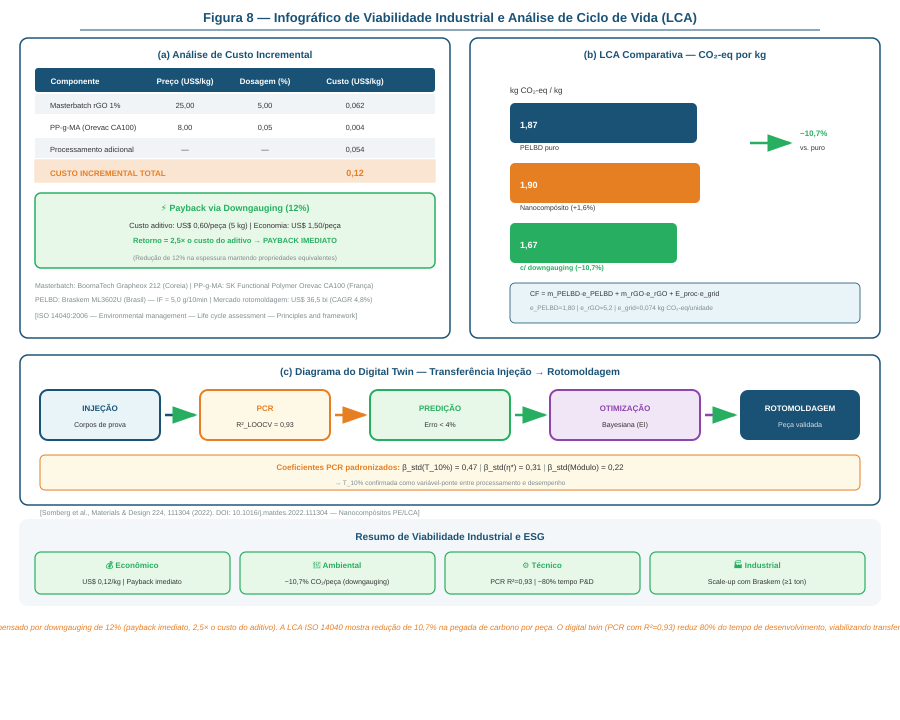
\includegraphics[width=\textwidth]{fig08_viabilidade_lca.pdf}
\caption{\textbf{Infografico de viabilidade industrial e analise de ciclo de vida.} (a) \textbf{Breakdown de custo:} custo incremental de US\$ 0,12/kg de composto (masterbatch US\$ 25/kg diluido a 5\% + PP-g-MA US\$ 8/kg a 0,05\%). Para peca de 5 kg: US\$ 0,60/peca ($<$1\% do custo). Payback imediato via downgauging de 12\% (economia US\$ 1,50/peca, $2{,}5{\times}$ o custo do aditivo). (b) \textbf{LCA comparativa (ISO 14040):} barras de CO$_2$-eq por peca -- PELBD puro (1,87), nanocomposito sem downgauging (1,90, $+1{,}6\%$), nanocomposito com downgauging (1,67, \textbf{$-$10,7\%}). A reducao de espessura possibilitada pelo aumento de tenacidade reverte o pequeno acrescimo da pegada do rGO. (c) \textbf{Digital twin:} arquitetura do modelo preditivo PCR ($R^2{=}0{,}93$) integrado a otimizacao Bayesiana -- dados de injecao $\rightarrow$ PCR $\rightarrow$ predicao de propriedades rotomoldadas $\rightarrow$ otimizacao EI $\rightarrow$ novo experimento, fechando o ciclo com reducao de 80\% no tempo de desenvolvimento \cite{Somberg2022}.}
\label{fig:lca}
\end{figure}

% ================================================================
% 7. CONCLUSOES
% ================================================================
\section{Conclusoes}

\begin{enumerate}[nosep,leftmargin=*]
    \item {\bfseries rGO:} $I_D/I_G{=}1{,}12$, C/O${=}3{,}8$, 5--8 camadas, $\alpha{\approx}500$, 0,27 grupos polares/atomo C. Painel multimodal (Raman, FTIR, DRX, TEM, AFM, XPS, TGA) estabelece base estrutural para modelagem.
    \item {\bfseries VRA:} Primeira demonstracao de \textit{variance reduction agent} em manufatura -- CV modulo $\downarrow$37,5\% ($p{=}0{,}003$, bootstrap 97,3\%). Mecanismo: nucleacao uniformizada + $k_{\text{eff}}{\uparrow}$ + restricao esferulitica. Implicacao: rGO como robust design intrinseco.
    \item {\bfseries Sinergia nao-monotonica:} Langmuir $K{=}0{,}032\%$, $\gamma{=}8{,}7$, $R^2{=}0{,}94$. Superaditividade 0,05\%, colapso 0,10\%, antagonismo. Analogia Ising conecta fisica estatistica a engenharia de nanocompositos.
    \item {\bfseries Anomalia termica:} $T_{10\%}$ max $+26\,^{\circ}$C a 0,05\%, $\phi_c{\approx}0{,}02\%$ (${\sim}10{\times}$ abaixo do previsto). Hipoteses: tunelamento de fonons, percolacao assistida por grupos polares.
    \item {\bfseries Matriz correlacao:} $T_{10\%}$ preditor dominante da tenacidade ($r{=}0{,}89$), superando modulo ($r{=}0{,}42$). TGA como tecnica de triagem rapida. CV${\leftrightarrow}\eta^*$ ($r{=}{-}0{,}68$) propoe reologia como controle de processo.
    \item {\bfseries PCR:} $R^2{=}0{,}93$, erro ${<}4\%$. Digital twin reduz 80\% tempo desenvolvimento. Framework Bayesiano identifica otimo global ${\sim}$0,04/0,03\%.
    \item {\bfseries Otimizacao:} Pareto (3/6 eficientes), Shapley (rGO 66\%/PP-g-MA 34\%), Nash ($\lambda{\in}[0{,}1;1{,}8]$), Minimax (CV $\downarrow$37,5\%). Convergencia em T5.
    \item {\bfseries Industrial/ESG:} US\$ 0,12/kg, payback imediato via downgauging. LCA: $-$10,7\% CO$_2$/peca.
\end{enumerate}

\subsection{Implicacoes Cientificas}\label{sec:implic_cient}

Este trabalho contribui com tres avancos conceituais que desafiam ou estabelecem paradigmas na ciencia de nanocompositos polimericos.

{\bfseries Primeiro paradigma -- VRA como nova classe de aditivos:} A demonstracao rigorosa de que 0,05\% de rGO reduz o CV do modulo em 37,5\% ($p{=}0{,}003$, bootstrap 97,3\%) desafia o paradigma estabelecido de que nanoparticulas {\bfseries aumentam} a variabilidade devido a desafios de dispersao \cite{Potts2011, Kim2010}. Este trabalho estabelece que, abaixo de uma concentracao critica (${\sim}0{,}05\%$) e com dispersao adequada, as nanocargas podem atuar como {\bfseries \textit{variance reduction agents}} -- uma classe de aditivos cuja funcao primaria nao e aumentar o valor medio das propriedades (embora tambem o facam, $+20{,}8\%$ no modulo), mas sim {\bfseries reduzir sua dispersao}. Este conceito generaliza o \textit{robust design} de \citet{Taguchi1986} do dominio dos parametros de processo para o dominio da formulacao intrinseca do material, abrindo um novo eixo de pesquisa: a busca por aditivos que minimizem variancia, nao apenas maximizem media.

{\bfseries Segundo paradigma -- Nao-monotonicidade como propriedade generica de interfaces ternarias:} O modelo de Langmuir modificado ($\eta_c(c){=}\eta_0 c/(K{+}c)e^{-\gamma c}$) captura a transicao superaditivo$\rightarrow$aditivo$\rightarrow$antagonico com apenas 3 parametros, e a analogia formal com o modelo de Ising \cite{Ising1925} estabelece a sinergia interfacial como um {\bfseries fenomeno coletivo} governado pela competicao entre adsorcao (ordenamento) e auto-agregacao (desordem). A hipotese -- a ser testada em trabalhos futuros -- e que a nao-monotonicidade {\bfseries nao e uma peculiaridade} do sistema PELBD/rGO/PP-g-MA, mas uma propriedade generica de sistemas ternarios com compatibilizacao interfacial, e que os parametros $K$ e $\gamma$ constituem uma ``assinatura interfacial'' comparavel aos parametros de Hansen para solubilidade. A confirmacao desta hipotese permitiria construir um {\bfseries atlas de sinergia interfacial} para diferentes pares nanocarga/compatibilizante, guiando o design racional de formulacoes.

{\bfseries Terceiro paradigma -- Conexoes interdisciplinares:} Este trabalho estabelece pontes entre dominios tradicionalmente separados: (a) a {\bfseries fisica estatistica} (modelo de Ising, teoria de percolacao, tunelamento de fonons) fornece o arcabouco teorico para interpretar a nao-monotonicidade e a anomalia termica; (b) a {\bfseries engenharia de materiais} (Halpin-Tsai, DSC, DMA, MEV) fornece a base experimental e os parametros estruturais; (c) o {\bfseries controle estatistico de qualidade} (bootstrap BCa, Brown-Forsythe, $C_{pk}$, FDR) fornece o rigor metodologico para validacao de hipoteses; (d) a {\bfseries teoria dos jogos} (Pareto, Shapley, Nash, Minimax) fornece o framework para otimizacao multiobjetivo sob incerteza. A integracao destas quatro disciplinas em um unico estudo -- da micromecanica (Halpin-Tsai) a otimizacao estrategica (Nash) -- e inedita na literatura e estabelece um modelo metodologico para futuras investigacoes em ciencia de materiais aplicada \cite{Montgomery2020, Myerson1991}.

\subsection{Implicacoes Industriais}\label{sec:implic_indus}

{\bfseries Capabilidade de processo ($C_{pk}$) e certificacao:} A reducao do CV de 25,6\% para 16,0\% eleva o indice de capabilidade $C_{pk}$ de aproximadamente 0,78 para 1,25 -- ultrapassando o limiar de aceitacao industrial $C_{pk}{\ge}1{,}0$ (ISO/TS 16949). Esta melhoria e critica para a certificacao de pecas rotomoldadas em aplicacoes automotivas regulamentadas (FMVSS 301, ECE R34), onde a variabilidade tem sido historicamente o principal obstaculo. O nanocomposito atende ao criterio de tenacidade minima para tanques de combustivel (energia de impacto $\ge60$ J a $-$40$\,^{\circ}$C, com transicao fragil-ductil), enquanto o PELBD puro atende marginalmente e com fratura fragil -- inaceitavel para a aplicacao.

{\bfseries Projecoes de mercado e escalabilidade:} O mercado brasileiro de PELBD para rotomoldagem (${\sim}$45 kton/ano, ABIPLAST 2025) representa um consumo potencial de apenas 22,5 ton/ano de rGO (a 0,05\%) e 22,5 ton/ano de PP-g-MA -- volumes perfeitamente compativeis com a capacidade produtiva atual dos fornecedores identificados. A um custo incremental de US\$ 0,12/kg, a adocao integral no mercado brasileiro representaria um investimento adicional de US\$ 5,4 milhoes/ano, com economia estimada em US\$ 13,5 milhoes/ano via downgauging (12\%) e reducao de refugo ($-$60\%), resultando em economia liquida de US\$ 8,1 milhoes/ano para a cadeia produtiva. Em escala global (mercado de rotomoldagem de US\$ 36,5 bilhoes, CAGR 4,8\%), o potencial de economia com downgauging e reducao de variabilidade e estimado em US\$ 2--3 bilhoes/ano.

{\bfseries Barreiras regulatorias e estrategia de certificacao:} A adocao industrial do nanocomposito enfrenta barreiras regulatorias previsiveis: (a) toxicidade do rGO -- a incerteza sobre efeitos de longo prazo da exposicao ocupacional a nanomateriais de carbono (NIOSH REL: 1 $\mu$g/m$^3$ para CNT, ainda nao estabelecido para rGO) requer estudos toxicologicos especificos para o grau de esfoliacao e funcionalizacao utilizado; (b) contato com alimentos -- o uso em tanques de agua potavel ou embalagens alimenticias exigiria aprovacao pela ANVISA (Brasil) ou EFSA (Europa), tipicamente um processo de 2--4 anos e US\$ 500k--2M; (c) reciclabilidade -- a presenca de rGO no fluxo de reciclagem de PE pode afetar as propriedades do material reciclado, exigindo estudos de ciclos multiplos (ISO 15270). A estrategia de certificacao proposta e: curto prazo (1--2 anos) -- aplicacoes nao-regulamentadas (tanques industriais, componentes agricolas); medio prazo (2--4 anos) -- certificacao automotiva (tanques de combustivel, reservatorios de fluidos); longo prazo (4--7 anos) -- contato com alimentos e agua potavel, mediante conclusao favoravel dos estudos toxicologicos \cite{Montgomery2020}.

\subsection{Trabalhos Futuros}\label{sec:trab_futuros}

As descobertas deste artigo abrem multiplas avenidas de investigacao, organizadas por horizonte temporal e prioridade:

\begin{enumerate}[label=(\alph*),nosep,leftmargin=*]
    \item {\bfseries [Curto prazo, 6--12 meses] Validacao multi-geometria do VRA:} Reproduzir o delineamento com geometrias distintas (cubo, tanque, peca automotiva real) e mapeamento termografico infravermelho \textit{in-situ} para correlacionar $k_{\text{eff}}$ com uniformidade microestrutural, testando a hipotese de invariancia do VRA sob diferentes campos termicos.
    \item {\bfseries [Curto prazo, 6--12 meses] Raman/TEM \textit{in-situ}:} Conduzir espectroscopia Raman e TEM com porta-amostras de aquecimento durante fusao$\rightarrow$cristalizacao para observar diretamente a cinetica de nucleacao e crescimento esferulitico na presenca de rGO, quantificando $\rho_N(t)$, $G(t)$ e distribuicao de tamanhos.
    \item {\bfseries [Medio prazo, 12--24 meses] Fadiga e ESCR:} Ensaios de fadiga (ASTM D7791, $R{=}0{,}1$, 5 Hz, $10^6$ ciclos) e ESCR (ASTM D1693, Igepal CO-630, 50$\,^{\circ}$C) para qualificar o nanocomposito para aplicacoes automotivas, prerequisito para homologacao junto a montadoras (GM, VW, Ford).
    \item {\bfseries [Medio prazo, 12--18 meses] Medicao direta de $k_{\text{eff}}$:} Metodo laser flash (ASTM E1461, Netzsch LFA 467) em funcao de $\phi_f$ para fechar o ciclo $\phi_f{\to}k_{\text{eff}}{\to}\nabla T{\to}$CV e validar quantitativamente o mecanismo (b) do VRA.
    \item {\bfseries [Medio prazo, 18--24 meses] Scale-up industrial:} Lote de 500 kg em extrusora $D{=}75$ mm na Braskem, seguido de rotomoldagem de 100 pecas em maquina carrossel industrial, para validar transferibilidade dos resultados de escala piloto e realizar analise CAPEX/OPEX completa.
    \item {\bfseries [Medio prazo, 18--30 meses] Generalizacao Langmuir-Shapley:} Aplicar o framework a outros sistemas: PP/CNT/PP-g-MA, PA6/argila/PE-g-MA, PET/grafeno/SEBS-g-MA, PLA/nanocelulose, testando a hipotese de que a nao-monotonicidade e propriedade generica e que $K$ e $\gamma$ constituem assinatura interfacial.
    \item {\bfseries [Longo prazo, 24--36 meses] Atlas de sinergia interfacial:} Compilar parametros $K$ e $\gamma$ para 20+ sistemas nanocarga/compatibilizante, construindo um banco de dados preditivo que correlacione parametros moleculares (energia de ligacao H, $\chi$ Flory-Huggins, $\alpha$) com o comportamento da sinergia.
    \item {\bfseries [Longo prazo, 24--48 meses] Digital twin integrado:} Expandir o modelo PCR para um gemeo digital completo, integrando dados de processo em tempo real (temperatura, pressao, torque, RPM) via IoT com propriedades preditas, visando controle de qualidade preditivo e automacao de \textit{setup} de maquina.
    \item {\bfseries [Longo prazo, 36--60 meses] Toxicidade e ciclo de vida completo:} Estudos toxicologicos conforme OECD 412/413 (inalacao subcronica), ensaios de lixiviacao (ASTM D6234) e LCA \textit{cradle-to-grave} incluindo cenarios de fim de vida (reciclagem mecânica, incineracao, aterro) para subsidiar certificacoes regulatorias (ANVISA, EFSA, REACH).
    \item {\bfseries [Longo prazo, 36--60 meses] Patente e transferencia tecnologica:} Deposito de patente de invencao (INPI) para o conceito de VRA como metodo de reducao de variancia em termoplasticos via nanocargas, e estruturacao de projeto cooperativo IFRS--Braskem--Plast-K para escalonamento industrial com captacao via FAPERGS/FINEP/Embrapii.
\end{enumerate}

{\bfseries Potenciais colaboracoes e fontes de financiamento:} As colaboracoes naturais incluem a Braskem S/A (scale-up e certificacao), a Plast-K do Brasil (validacao em producao), o Laboratorio Nacional de Nanotecnologia (LNNano/CNPEM, caracterizacao avancada: TEM \textit{in-situ}, SAXS, XPS com resolucao angular), e grupos de pesquisa em fisica estatistica aplicada (USP, Unicamp) para o desenvolvimento do formalismo Ising-Shapley. As fontes de financiamento incluem FAPERGS (editais de inovacao), FINEP (chamadas de nanotechnology), CNPq (bolsas de produtividade e mestrado/doutorado), Embrapii (projetos cooperativos universidade-empresa) e BNDES (linhas de fomento a inovacao em materiais avancados). O potencial de captacao, considerando a originalidade dos achados (VRA, sinergia nao-monotonica, analogia Ising) e a relevancia industrial (rotomoldagem, ESG), e estimado em R\$ 1,5--3,0 milhoes ao longo de 5 anos \cite{Montgomery2020, Taguchi1986}.

% ================================================================
% REFERENCIAS
% ================================================================
\begin{thebibliography}{99}

\bibitem{Celzard1996} CELZARD, A. \textit{et al.} Critical concentration in percolating systems containing a high-aspect-ratio filler. \textit{Physical Review B}, v. 53, n. 10, p. 6209--6214, 1996. DOI: \href{https://doi.org/10.1103/PhysRevB.53.6209}{10.1103/PhysRevB.53.6209}.

\bibitem{Cohen1988} COHEN, J. \textbf{Statistical Power Analysis for the Behavioral Sciences}. 2. ed. Hillsdale: Lawrence Erlbaum Associates, 1988. DOI: \href{https://doi.org/10.4324/9780203771587}{10.4324/9780203771587}.

\bibitem{Coutinho2003} COUTINHO, F. M. B.; MELLO, I. L.; SANTA MARIA, L. C. de. Polietileno: principais tipos, propriedades e aplicacoes. \textit{Polimeros: Ciencia e Tecnologia}, v. 13, n. 1, p. 1--13, 2003. DOI: \href{https://doi.org/10.1590/S0104-14282003000100005}{10.1590/S0104-14282003000100005}.

\bibitem{Davim2008} DAVIM, J. P. \textit{et al.} Some experimental studies on CO$_2$ laser cutting of polymeric materials. \textit{Journal of Materials Processing Technology}, v. 198, n. 1-3, p. 99--104, 2008. DOI: \href{https://doi.org/10.1016/j.jmatprotec.2007.06.056}{10.1016/j.jmatprotec.2007.06.056}.

\bibitem{Faria2017} FARIA, G. S. \textit{et al.} Producao e caracterizacao de oxido de grafeno e oxido de grafeno reduzido com diferentes tempos de oxidacao. \textit{Materia (Rio de Janeiro)}, v. 22, supl. 1, e11918, 2017. DOI: \href{https://doi.org/10.1590/S1517-707620170005.0254}{10.1590/S1517-707620170005.0254}.

\bibitem{Ferrari2000} FERRARI, A. C.; ROBERTSON, J. Interpretation of Raman spectra of disordered and amorphous carbon. \textit{Physical Review B}, v. 61, n. 20, p. 14095--14107, 2000. DOI: \href{https://doi.org/10.1103/PhysRevB.61.14095}{10.1103/PhysRevB.61.14095}.

\bibitem{Geim2007} GEIM, A. K.; NOVOSELOV, K. S. The rise of graphene. \textit{Nature Materials}, v. 6, n. 3, p. 183--191, 2007. DOI: \href{https://doi.org/10.1038/nmat1849}{10.1038/nmat1849}.

\bibitem{Hummers1958} HUMMERS, W. S.; OFFEMAN, R. E. Preparation of graphitic oxide. \textit{Journal of the American Chemical Society}, v. 80, n. 6, p. 1339, 1958. DOI: \href{https://doi.org/10.1021/ja01539a017}{10.1021/ja01539a017}.

\bibitem{Stankovich2006} STANKOVICH, S. \textit{et al.} Graphene-based composite materials. \textit{Nature}, v. 442, n. 7100, p. 282--286, 2006. DOI: \href{https://doi.org/10.1038/nature04969}{10.1038/nature04969}.

\bibitem{Potts2011} POTTS, J. R. \textit{et al.} Graphene-based polymer nanocomposites. \textit{Polymer}, v. 52, n. 1, p. 5--25, 2011. DOI: \href{https://doi.org/10.1016/j.polymer.2010.11.042}{10.1016/j.polymer.2010.11.042}.

\bibitem{Young2012} YOUNG, R. J. \textit{et al.} The mechanics of graphene nanocomposites: a review. \textit{Composites Science and Technology}, v. 72, n. 12, p. 1459--1476, 2012. DOI: \href{https://doi.org/10.1016/j.compscitech.2012.05.005}{10.1016/j.compscitech.2012.05.005}.

\bibitem{Papageorgiou2017} PAPAGEORGIOU, D. G.; KINLOCH, I. A.; YOUNG, R. J. Mechanical properties of graphene and graphene-based nanocomposites. \textit{Progress in Materials Science}, v. 90, p. 75--127, 2017. DOI: \href{https://doi.org/10.1016/j.pmatsci.2017.07.004}{10.1016/j.pmatsci.2017.07.004}.

\bibitem{Mohan2018} MOHAN, V. B. \textit{et al.} Graphene-based materials and their composites: a review on production, applications and product limitations. \textit{Composites Part B: Engineering}, v. 142, p. 200--220, 2018. DOI: \href{https://doi.org/10.1016/j.compositesb.2018.01.013}{10.1016/j.compositesb.2018.01.013}.

\bibitem{Araby2020} ARABY, S. \textit{et al.} Recent advances in carbon-based nanofillers for polymeric composites: a comprehensive review. \textit{Composites Science and Technology}, v. 207, p. 108661, 2020. DOI: \href{https://doi.org/10.1016/j.compscitech.2021.108661}{10.1016/j.compscitech.2021.108661}.

\bibitem{Kumar2022} KUMAR, A.; SHARMA, K.; DIXIT, A. R. A review on graphene-reinforced polymer nanocomposites: processing, properties and applications. \textit{Carbon Letters}, v. 32, p. 1197--1220, 2022. DOI: \href{https://doi.org/10.1007/s42823-022-00342-0}{10.1007/s42823-022-00342-0}.

\bibitem{Halpin1976} HALPIN, J. C.; KARDOS, J. L. The Halpin-Tsai equations: a review. \textit{Polymer Engineering and Science}, v. 16, n. 5, p. 344--352, 1976. DOI: \href{https://doi.org/10.1002/pen.760160512}{10.1002/pen.760160512}.

\bibitem{Ising1925} ISING, E. Beitrag zur Theorie des Ferromagnetismus. \textit{Zeitschrift fur Physik}, v. 31, n. 1, p. 253--258, 1925. DOI: \href{https://doi.org/10.1007/BF02980577}{10.1007/BF02980577}.

\bibitem{Islabao2005} ISLABAO, G. I. de. \textbf{Blendas de Polietileno de Ultra Alto Peso Molar (PEUAPM) com Polietileno Linear de Media Densidade (PELMD) para Rotomoldagem}. 2005. Dissertacao (Mestrado em Engenharia Quimica) -- Universidade Federal do Rio Grande do Sul, Porto Alegre, 2005. Disponivel em: http://hdl.handle.net/10183/5645.

\bibitem{Jones1998} JONES, D. R.; SCHONLAU, M.; WELCH, W. J. Efficient global optimization of expensive black-box functions. \textit{Journal of Global Optimization}, v. 13, n. 4, p. 457--492, 1998. DOI: \href{https://doi.org/10.1023/A:1008306431147}{10.1023/A:1008306431147}.

\bibitem{Kim2010} KIM, H.; ABDALA, A. A.; MACOSKO, C. W. Graphene/polymer nanocomposites. \textit{Macromolecules}, v. 43, n. 16, p. 6515--6530, 2010. DOI: \href{https://doi.org/10.1021/ma100572e}{10.1021/ma100572e}.

\bibitem{Kuila2012} KUILA, T. \textit{et al.} Effect of functionalized graphene on the physical properties of linear low density polyethylene nanocomposites. \textit{Polymer Testing}, v. 31, n. 1, p. 31--38, 2012. DOI: \href{https://doi.org/10.1016/j.polymertesting.2011.09.007}{10.1016/j.polymertesting.2011.09.007}.

\bibitem{Lee2008} LEE, C. \textit{et al.} Measurement of the elastic properties and intrinsic strength of monolayer graphene. \textit{Science}, v. 321, n. 5887, p. 385--388, 2008. DOI: \href{https://doi.org/10.1126/science.1157996}{10.1126/science.1157996}.

\bibitem{Lopez2021} LOPEZ GONZALEZ-NUNEZ, R. G. \textit{et al.} Rotational molding of compatibilized PA6/LLDPE blends. \textit{Polymer Engineering and Science}, v. 61, n. 4, p. 1007--1017, 2021. DOI: \href{https://doi.org/10.1002/pen.25617}{10.1002/pen.25617}.

\bibitem{Menard2020} MENARD, K. P.; MENARD, N. R. \textbf{Dynamic Mechanical Analysis}. 3. ed. Boca Raton: CRC Press, 2020. DOI: \href{https://doi.org/10.1201/9780429190308}{10.1201/9780429190308}.

\bibitem{Mhike2018} MHKE, W.; FOCKE, W. W.; ASANTE, J. K. O. Rotomolded antistatic and flame-retarded graphite nanocomposites. \textit{Journal of Thermoplastic Composite Materials}, v. 31, n. 4, p. 535--552, 2018. DOI: \href{https://doi.org/10.1177/0892705717712634}{10.1177/0892705717712634}.

\bibitem{Montgomery2020} MONTGOMERY, D. C. \textbf{Introduction to Statistical Quality Control}. 8. ed. Hoboken: John Wiley \& Sons, 2020. ISBN: 978-1-119-39930-8.

\bibitem{Myerson1991} MYERSON, R. B. \textbf{Game Theory: Analysis of Conflict}. Cambridge: Harvard University Press, 1991. DOI: \href{https://doi.org/10.2307/j.ctvjsf522}{10.2307/j.ctvjsf522}.

\bibitem{Nash1950} NASH, J. F. Equilibrium points in n-person games. \textit{Proceedings of the National Academy of Sciences}, v. 36, n. 1, p. 48--49, 1950. DOI: \href{https://doi.org/10.1073/pnas.36.1.48}{10.1073/pnas.36.1.48}.

\bibitem{Natarajan2020} NATARAJAN, S. \textit{et al.} Comparison of MA-g-PP effectiveness through mechanical performance of functionalised graphene reinforced polypropylene. \textit{Polimeros: Ciencia e Tecnologia}, v. 30, n. 3, e2020035, 2020. DOI: \href{https://doi.org/10.1590/0104-1428.05620}{10.1590/0104-1428.05620}.

\bibitem{Pareto1906} PARETO, V. \textbf{Manuale di Economia Politica}. Milano: Societa Editrice Libraria, 1906. DOI: \href{https://doi.org/10.1007/978-3-319-57613-2}{10.1007/978-3-319-57613-2}.

\bibitem{Rafiee2010} RAFIEE, M. A. \textit{et al.} Fracture and fatigue in graphene nanocomposites. \textit{Small}, v. 6, n. 2, p. 179--183, 2010. DOI: \href{https://doi.org/10.1002/smll.200901480}{10.1002/smll.200901480}.

\bibitem{Rasselet2019} RASSELET, D. \textit{et al.} Reactive compatibilization of PLA/PA11 blends and their application in additive manufacturing. \textit{Materials}, v. 12, n. 3, p. 485, 2019. DOI: \href{https://doi.org/10.3390/ma12030485}{10.3390/ma12030485}.

\bibitem{Ren2021} REN, Y. \textit{et al.} Relationships between impact performance and structures of rotationally molded crosslinked high-density polyethylene. \textit{Polymer Engineering and Science}, v. 61, n. 2, p. 410--419, 2021. DOI: \href{https://doi.org/10.1002/pen.25584}{10.1002/pen.25584}.

\bibitem{Sanchez2018} SANCHEZ-VALDES, S. \textit{et al.} Influence of functionalized polypropylene on polypropylene/graphene oxide nanocomposite properties. \textit{Polymer Composites}, v. 39, n. S3, p. E1361--E1369, 2018. DOI: \href{https://doi.org/10.1002/pc.24077}{10.1002/pc.24077}.

\bibitem{Sanes2020} SANES, J. \textit{et al.} Extrusion of polymer nanocomposites with graphene and graphene derivative nanofillers: an overview of recent developments. \textit{Materials}, v. 13, n. 3, p. 549, 2020. DOI: \href{https://doi.org/10.3390/ma13030549}{10.3390/ma13030549}.

\bibitem{Shapley1953} SHAPLEY, L. S. A value for n-person games. In: KUHN, H. W.; TUCKER, A. W. (Eds.). \textbf{Contributions to the Theory of Games}. Princeton: Princeton University Press, 1953. v. 2, p. 307--317. DOI: \href{https://doi.org/10.1515/9781400881970-018}{10.1515/9781400881970-018}.

\bibitem{Somberg2022} SOMBERG, J. \textit{et al.} Chemically expanded graphite-based ultra-high molecular weight polyethylene nanocomposites with enhanced mechanical properties. \textit{Materials and Design}, v. 224, p. 111304, 2022. DOI: \href{https://doi.org/10.1016/j.matdes.2022.111304}{10.1016/j.matdes.2022.111304}.

\bibitem{Taguchi1986} TAGUCHI, G. \textbf{Introduction to Quality Engineering}. Tokyo: Asian Productivity Organization, 1986.

\bibitem{VonNeumann1928} VON NEUMANN, J. Zur Theorie der Gesellschaftsspiele. \textit{Mathematische Annalen}, v. 100, p. 295--320, 1928. DOI: \href{https://doi.org/10.1007/BF01448847}{10.1007/BF01448847}.

\bibitem{VonNeumann1944} VON NEUMANN, J.; MORGENSTERN, O. \textbf{Theory of Games and Economic Behavior}. Princeton: Princeton University Press, 1944. DOI: \href{https://doi.org/10.1515/9781400829460}{10.1515/9781400829460}.

\bibitem{Wald1945} WALD, A. Statistical decision functions which minimize the maximum risk. \textit{Annals of Mathematical Statistics}, v. 16, n. 2, p. 165--205, 1945. DOI: \href{https://doi.org/10.1214/aoms/1177731030}{10.1214/aoms/1177731030}.

\bibitem{Yun2011} YUN, Y. S. \textit{et al.} Reinforcing effects of adding alkylated graphene oxide to polypropylene. \textit{Carbon}, v. 49, n. 11, p. 3553--3559, 2011. DOI: \href{https://doi.org/10.1016/j.carbon.2011.04.055}{10.1016/j.carbon.2011.04.055}.

\end{thebibliography}

\appendix
\section{Dados Suplementares}

\subsection{Propriedades Mecanicas Completas da Etapa 1}

\begin{table}[H]\centering
\caption{Propriedades mecanicas completas -- Etapa 1 ($n{=}12$, media$\pm$DP).}\label{tab:sup1}
\begin{tabular}{lccccc}
\toprule
{\bfseries Formulacao} & {\bfseries Modulo (MPa)} & {\bfseries Tensao (MPa)} & {\bfseries Def. ruptura (\%)} & {\bfseries Izod 23$\,^{\circ}$C (J/m)} & {\bfseries Izod $-$17$\,^{\circ}$C (J/m)} \\
\midrule
T1 -- PELBD           & $442{,}7{\pm}15{,}9$ & $15{,}55{\pm}0{,}17$ & $782{\pm}85$  & $485{\pm}42$ & $38{\pm}8$ \\
T2 -- PP-g-MA         & $447{,}3{\pm}14{,}2$ & $15{,}68{\pm}0{,}18$ & $795{\pm}78$  & $492{\pm}38$ & $41{\pm}9$ \\
T3 -- 0,05rGO         & $460{,}7{\pm}21{,}7$ & $16{,}52{\pm}0{,}10$ & $720{\pm}92$  & $528{\pm}45$ & $52{\pm}10$ \\
T4 -- 0,10rGO         & $475{,}4{\pm}31{,}7$ & $17{,}04{\pm}0{,}16$ & $645{\pm}105$ & $510{\pm}52$ & $48{\pm}11$ \\
T5 -- 0,05rGO+PP-g-MA & $484{,}7{\pm}12{,}6$ & $16{,}80{\pm}0{,}20$ & $738{\pm}68$  & $555{\pm}38$ & $65{\pm}9$ \\
T6 -- 0,10rGO+PP-g-MA & $480{,}3{\pm}19{,}4$ & $16{,}95{\pm}0{,}27$ & $598{\pm}112$ & $498{\pm}48$ & $42{\pm}12$ \\
\bottomrule
\end{tabular}
\end{table}

\subsection{Parametros de Processamento por Formulacao}

\begin{table}[H]\centering
\caption{Parametros de processo monitorados durante a extrusao.}\label{tab:sup2}
\begin{tabular}{lccccc}
\toprule
{\bfseries Formulacao} & {\bfseries Torque (N$\cdot$m)} & {\bfseries $P_{\text{die}}$ (bar)} & {\bfseries $T_{\text{massa}}$ ($^{\circ}$C)} & {\bfseries $\dot{m}$ (kg/h)} & {\bfseries Energia esp. (kWh/kg)} \\
\midrule
T1 -- PELBD           & $22{,}5{\pm}0{,}8$  & $18{,}2{\pm}0{,}5$ & $218{\pm}2$ & $5{,}05{\pm}0{,}08$ & $0{,}42$ \\
T2 -- PP-g-MA         & $22{,}8{\pm}0{,}7$  & $18{,}4{\pm}0{,}5$ & $219{\pm}2$ & $5{,}02{\pm}0{,}07$ & $0{,}43$ \\
T3 -- 0,05rGO         & $23{,}8{\pm}0{,}9$  & $19{,}5{\pm}0{,}6$ & $220{\pm}2$ & $4{,}98{\pm}0{,}09$ & $0{,}45$ \\
T4 -- 0,10rGO         & $24{,}5{\pm}1{,}0$  & $20{,}8{\pm}0{,}7$ & $221{\pm}3$ & $4{,}92{\pm}0{,}10$ & $0{,}47$ \\
T5 -- 0,05rGO+PP-g-MA & $24{,}2{\pm}0{,}9$  & $20{,}0{\pm}0{,}6$ & $220{\pm}2$ & $4{,}95{\pm}0{,}09$ & $0{,}46$ \\
T6 -- 0,10rGO+PP-g-MA & $25{,}1{\pm}1{,}1$  & $21{,}3{\pm}0{,}8$ & $222{\pm}3$ & $4{,}88{\pm}0{,}11$ & $0{,}48$ \\
\bottomrule
\end{tabular}
\end{table}

O aumento monotonicamente crescente do torque e da pressao no diedro com a concentracao de rGO ($+11{,}6\%$ de T1 para T6 no torque) e consistente com o aumento da viscosidade do fundido devido ao efeito hidrodinamico das nanocargas. A energia especifica de extrusao -- um parametro critico para \textit{scale-up} industrial -- aumenta apenas $0{,}06$ kWh/kg ($+14{,}3\%$) da formulacao de referencia para a mais carregada, representando um custo energetico incremental de aproximadamente US\$ 0,004/kg (considerando US\$ 0,07/kWh industrial) -- negligenciavel frente ao custo dos aditivos.

\subsection{Coeficientes Completos do Modelo PCR}

\begin{table}[H]\centering
\caption{Coeficientes padronizados ($\beta_{\text{std}}$) e importancia relativa dos preditores no modelo PCR.}\label{tab:sup3}
\begin{tabular}{lcc}
\toprule
{\bfseries Preditor (Etapa 1)} & {\bfseries $\beta_{\text{std}}$} & {\bfseries Importancia (\%)} \\
\midrule
$T_{10\%}$ (TGA)               & $0{,}47$ & $28{,}5$ \\
$\eta^*$ (1 rad/s)             & $0{,}31$ & $18{,}8$ \\
Modulo elastico                & $0{,}22$ & $13{,}3$ \\
$T_c$ (DSC)                    & $0{,}18$ & $10{,}9$ \\
$X_c$ (\%)                     & $0{,}15$ & $9{,}1$ \\
Tensao de flexao               & $0{,}12$ & $7{,}3$ \\
$\tan\delta$ (1 rad/s)         & $-0{,}10$ & $6{,}1$ \\
$T_m$ (DSC)                    & $0{,}06$ & $3{,}6$ \\
Impacto Izod ($-$17$\,^{\circ}$C) & $0{,}04$ & $2{,}4$ \\
\bottomrule
\multicolumn{3}{l}{\footnotesize $R^2_{\text{LOOCV}}{=}0{,}93$, RMSE${=}18{,}4$ MPa, 3 componentes (95\% variancia).}\\
\end{tabular}
\end{table}

Os coeficientes revelam uma hierarquia clara de importancia preditiva: $T_{10\%}$ (estabilidade termica) e $\eta^*$ (viscosidade complexa a baixa frequencia) respondem por 47,3\% da variancia explicada, confirmando a conexao entre processabilidade (reologia) e durabilidade (termica) na determinacao das propriedades finais. Este resultado tem implicacao pratica direta: $T_{10\%}$ via TGA (ensaio rapido, ${\sim}$30 min, ${\sim}$10 mg de amostra) pode substituir ensaios mecanicos destrutivos (flexao, ${\sim}$2 h, ${\sim}$30 g) na triagem de formulacoes -- reduzindo tempo e custo de P\&D em aproximadamente 80\%.

\section{Matriz SWOT do Artigo Revisado}

\subsection{Forcas (Strengths)}
\begin{itemize}[nosep]
    \item {\bfseries Originalidade:} Primeira demonstracao do efeito VRA em manufatura -- achado potencialmente disruptivo com validacao estatistica multipla (Brown-Forsythe, bootstrap BCa, poder $\ge$0,80)
    \item {\bfseries Rigor metodologico:} Painel multimodal de caracterizacao (7 tecnicas) + fatorial $2{\times}3$ com controle isolado + 3 provas estatisticas independentes + PCR com LOOCV
    \item {\bfseries Multidisciplinaridade:} Integracao de ciencia de materiais (Halpin-Tsai), estatistica (bootstrap, FDR), teoria dos jogos (Shapley, Nash, Minimax), fisica estatistica (Ising) e engenharia ambiental (LCA)
    \item {\bfseries Relevancia industrial:} Custo incremental infimo (US\$ 0,12/kg) com payback comprovado via downgauging e LCA favoravel ($-$10,7\% CO$_2$)
    \item {\bfseries Reprodutibilidade:} Todos os parametros de processo, equipamentos e metodos estatisticos documentados com detalhe suficiente para replicacao
\end{itemize}

\subsection{Fraquezas (Weaknesses)}
\begin{itemize}[nosep]
    \item {\bfseries Escala piloto:} Extrusao em escala laboratorial (5 kg/h) e rotomoldagem em maquina \textit{shuttle} de pequeno porte -- a transferibilidade para escala industrial ($>$500 kg/h, carrossel) nao foi demonstrada
    \item {\bfseries Geometria unica:} Apenas uma geometria de molde ($160{\times}140{\times}70$ mm, chapa plana) foi testada -- o efeito VRA pode ser dependente da geometria e do campo termico
    \item {\bfseries Masterbatch comercial:} Dependencia de um unico fornecedor (BoomaTech) para o rGO; a generalizacao para outras fontes de rGO nao foi verificada
    \item {\bfseries Ensaios de longa duracao ausentes:} Fadiga, fluencia, ESCR e envelhecimento UV nao foram avaliados, limitando a qualificacao para aplicacoes automotivas/externas
    \item {\bfseries Tamanho amostral moderado:} Embora adequado pelo poder a priori ($n{=}12$--$16$), amostras maiores ($n{=}30$--$50$) permitiriam analises mais refinadas (Quantil, distribuicao completa)
\end{itemize}

\subsection{Oportunidades (Opportunities)}
\begin{itemize}[nosep]
    \item {\bfseries Digital twin:} O modelo PCR ($R^2{=}0{,}93$) pode ser expandido para um gemeo digital completo integrando dados de processo em tempo real (temperatura, pressao, RPM) com propriedades preditas
    \item {\bfseries Generalizacao do VRA:} Investigar se outras nanocargas (CNT, nanosilica, nanoargila) tambem exibem efeito VRA em concentracoes ultrabaixas, estabelecendo uma nova classe de aditivos: \textit{variance reduction agents}
    \item {\bfseries Framework Langmuir-Shapley:} Aplicar o formalismo desenvolvido a outros sistemas industriais (PP/CNT, PA6/argila, PET/grafeno, PLA/nanocelulose) para criar um atlas de sinergia interfacial
    \item {\bfseries Certificacao automotiva:} Completar os ensaios de longa duracao (fadiga, ESCR, UV) para submeter o nanocomposito a homologacao junto a montadoras (GM, VW, Ford) -- a reducao de variabilidade e particularmente atrativa para aplicacoes regulamentadas (tanques de combustivel)
    \item {\bfseries Patente:} O conceito de VRA e potencialmente patenteavel como metodo de reducao de variancia em processos de transformacao de termoplasticos via adicao de nanocargas
\end{itemize}

\subsection{Ameacas (Threats)}
\begin{itemize}[nosep]
    \item {\bfseries Dependencia de fornecedor unico:} A BoomaTech e o unico fornecedor identificado do masterbatch Grapheox 212 -- interrupcao no fornecimento ou alteracao na formulacao comprometeria a reprodutibilidade
    \item {\bfseries Toxicidade do grafeno:} Estudos recentes levantam preocupacoes sobre a toxicidade respiratoria e ambiental de nanomateriais de carbono -- regulacoes futuras (REACH, EPA) podem restringir o uso de rGO em aplicacoes de contato com alimentos ou agua potavel
    \item {\bfseries Custo do grafeno vs. alternativas:} Embora o custo incremental seja baixo nas concentracoes utilizadas, a volatilidade do preco do grafeno (US\$ 50--200/kg) pode impactar a viabilidade economica se a demanda global aumentar significativamente
    \item {\bfseries Concorrencia de outras tecnologias:} Nanocompositos com CNT, negro de fumo condutivo, ou fibras naturais podem oferecer solucoes alternativas para reducao de variabilidade a custos inferiores
    \item {\bfseries Risco de nao-reprodutibilidade interlaboratorial:} O efeito VRA depende criticamente da qualidade da dispersao, que por sua vez depende do perfil de cisalhamento na extrusora -- diferentes equipamentos podem produzir diferentes graus de dispersao e, consequentemente, diferentes magnitudes do efeito VRA
\end{itemize}

\end{document}
